  %  \nonstopmode
\documentclass[10pt,letterpaper,cm]{nupset}
\usepackage[margin=1in]{geometry}
\usepackage{graphicx}
\usepackage{enumerate}
\usepackage{enumitem}
\usepackage{float}
\usepackage{stmaryrd}
\usepackage{bm}
\usepackage{amsfonts}
\usepackage{amssymb}
\usepackage{mathtools}
\usepackage{upgreek}
\usepackage{pgfplots}
\pgfplotsset{compat=1.13}
\usepackage{amsmath,amsthm}
\usepackage{tikz-cd}
\usetikzlibrary{positioning, shapes.geometric}
\usetikzlibrary{knots,calc}
\usepackage{xcolor}
\usepackage{soul}
\usetikzlibrary{decorations.markings}
\usepackage{faktor}
\usepackage{xfrac}
\usepackage{ mathrsfs }
\usepackage{hyperref}
\hypersetup{colorlinks=true, linkcolor=red,          % color of internal links (change box color with linkbordercolor)
    citecolor=green,        % color of links to bibliography
    filecolor=magenta,      % color of file links
    urlcolor=cyan           }
\usepackage{adjustbox}
\usepackage{ bbold }
\usepackage{media9}
\usepackage{ifthen}
\usetikzlibrary{shapes.geometric}
\usetikzlibrary{decorations, decorations.markings} 
\usetikzlibrary{arrows, arrows.meta}
\tikzset{ ->-/.style args={#1 #2 #3}{
         decoration={markings,mark= at position 0.5 with {\arrow{stealth}}, }, 
            postaction={decorate}, }, 
        ->-/.default= {0.5 6pt black }}
\tikzset{ -<-/.style args={#1 #2 #3}{
        decoration={markings,mark= at position 0.5 with {\arrow[>=stealth]{<}}, }, 
        postaction={decorate}, }, 
    -<-/.default= {0.5 6pt black }}

\usepackage{thmtools}
\usepackage[capitalise]{cleveref} 
    
\theoremstyle{definition}
\newtheorem{definition}{Definition}[subsection]
\newtheorem{exmp}[definition]{Example}
\newtheorem{non-exmp}[definition]{Non-example}
\newtheorem{note}[definition]{Note}

\theoremstyle{theorem}
\newtheorem{theorem}[definition]{Theorem}
\newtheorem{lemma}[definition]{Lemma}
\newtheorem{prop}[definition]{Proposition}
\newtheorem{corollary}[definition]{Corollary}
\newtheorem*{claim}{Claim}
\newtheorem{exercise}[definition]{Exercise}

\theoremstyle{remark}
\newtheorem{remark}[definition]{Remark}
\newtheorem*{todo}{To do}
\newtheorem*{question}{Question}
\newtheorem*{conv}{Convention}
\newtheorem*{aside}{Aside}
\newtheorem*{notation}{Notation}
\newtheorem*{term}{Terminology}
\newtheorem*{background}{Background}
\newtheorem*{further}{Further reading}
\newtheorem*{sources}{Sources}

\makeatletter
\def\th@plain{%
  \thm@notefont{}% same as heading font
  \itshape % body font
}
\def\th@definition{%
  \thm@notefont{}% same as heading font
  \normalfont % body font
}
\makeatother


\makeatletter
\renewcommand*\env@matrix[1][*\c@MaxMatrixCols c]{%
  \hskip -\arraycolsep
  \let\@ifnextchar\new@ifnextchar
  \array{#1}}
\makeatother
\pgfplotsset{unit circle/.style={width=4cm,height=4cm,axis lines=middle,xtick=\empty,ytick=\empty,axis equal,enlargelimits,xmax=1,ymax=1,xmin=-1,ymin=-1,domain=0:pi/2}}
\DeclareMathOperator{\Ima}{Im}
\newcommand{\A}{\mathcal A}
\newcommand{\C}{\mathbb C}
\newcommand{\E}{\vec E}
\newcommand{\CP}{\mathbb{CP}}
\newcommand{\F}{\mathbb F}
\newcommand{\G}{\vec G}
\renewcommand{\H}{\mathbb H}
\newcommand{\HP}{\mathbb HP}
\newcommand{\K}{\mathbb K}
\renewcommand{\L}{\mathscr L}
\newcommand{\N}{\mathbb N}
\renewcommand{\O}{\mathbf O}
\newcommand{\OP}{\mathbb OP}
\renewcommand{\P}{\mathcal P}
\newcommand{\Q}{\mathbb Q}
\newcommand{\U}{\mathcal U}
\newcommand{\I}{\mathbb I}
\newcommand{\R}{\mathbb{R}}
\newcommand{\RP}{\mathbb{RP}}
\renewcommand{\S}{\mathbb S}
\newcommand{\T}{\mathcal T}
\newcommand{\X}{\mathbf X}
\newcommand{\Z}{\mathbb Z}
\newcommand{\B}{\mathbb{B}}
\newcommand{\1}{\mathbb{1}}
\newcommand{\ds}{\displaystyle}
\newcommand{\ran}{\right>}
\newcommand{\lan}{\left<}
\newcommand{\bmat}[1]{\begin{bmatrix} #1 \end{bmatrix}}
\renewcommand{\a}{\vec{a}}
\renewcommand{\b}{\vec b}
\renewcommand{\c}{\vec c}
\renewcommand{\d}{\vec d}
\newcommand{\e}{\vec e}
\newcommand{\h}{\vec h}
\newcommand{\f}{\vec f}
\newcommand{\g}{\vec g}
\renewcommand{\i}{\vec i}
\renewcommand{\j}{\vec j}
\renewcommand{\k}{\vec k}
\newcommand{\n}{\vec n}
\newcommand{\p}{\vec p}
\newcommand{\q}{\vec q}
\renewcommand{\r}{\vec r}
\newcommand{\s}{\vec s}
\renewcommand{\t}{\vec t}
\renewcommand{\u}{\vec u}
\newcommand{\w}{\vec w}
\newcommand{\x}{\vec x}
\newcommand{\y}{\vec y}
\newcommand{\z}{\vec z}
\newcommand{\0}{\vec 0}
\newcommand{\pt}{\mathsf{pt}}

\newcommand{\cw}{\mathrm{CW}}

\newcommand{\from}{\longleftarrow}
\newcommand{\intprodl}{%
    \mathbin{\scalebox{1.5}{$\lrcorner$}}%
}
\newcommand{\intprodr}{%
    \mathbin{\scalebox{1.5}{$\llcorner$}}%
}
\DeclareMathOperator*{\Span}{span}
\DeclareMathOperator{\rng}{range}
\DeclareMathOperator{\gemu}{gemu}
\DeclareMathOperator{\almu}{almu}
\newcommand{\Char}{\mathsf{char}}
\DeclareMathOperator{\id}{id}
\DeclareMathOperator{\tr}{Tr}
\DeclareMathOperator{\tor}{Tor}
\DeclareMathOperator{\im}{im}
\DeclareMathOperator{\homeo}{Homeo}
\DeclareMathOperator{\GL}{GL}
\DeclareMathOperator{\SL}{SL}
\DeclareMathOperator{\norm}{N}
\DeclareMathOperator{\aut}{Aut}
\DeclareMathOperator{\Int}{Int}
\DeclareMathOperator{\ext}{Ext}
\DeclareMathOperator{\M}{M}
\DeclareMathOperator{\supp}{supp}
\DeclareMathOperator{\cl}{cl}
\DeclareMathOperator{\dom}{dom}
\DeclareMathOperator{\rnk}{rank}
\DeclareMathOperator{\Hom}{Hom}
\DeclareMathOperator{\Alt}{Alt}
\DeclareMathOperator{\dr}{dR}
\DeclareMathOperator{\ed}{End}
\DeclareMathOperator{\BM}{BM}
\DeclareMathOperator{\ob}{ob}
\DeclareMathOperator{\clength}{cup{-}length}
\DeclareMathOperator{\sgn}{sgn}
\DeclareMathOperator{\orb}{Orb}
\DeclareMathOperator{\cyl}{Cyl}
\DeclareMathOperator{\rel}{rel}
\DeclareMathOperator{\cat}{cat}
\DeclareMathOperator{\op}{op}
\DeclareMathOperator{\Gd}{Gd}
\DeclareMathOperator{\coker}{coker}
\DeclareMathOperator{\map}{Map}
\DeclareMathOperator{\sing}{Sing}
\DeclareMathOperator{\Op}{\mathbf{Op}}
\DeclareMathOperator{\colim}{colim}
\DeclareMathOperator{\tot}{Tot}
\DeclareMathOperator{\Et}{\acute{E}t}
\DeclareMathOperator{\ch}{\mathbf{Ch}}
\DeclareMathOperator{\vf}{\mathscr{X}}

\newcommand{\midarrow}{\tikz \draw[-triangle 90] (0,0) -- +(.1,0);}

\newcommand{\mathcolorbox}[2]{\colorbox{#1}{$\displaystyle #2$}}

\newlist{steps}{enumerate}{1}
\setlist[steps, 1]{label = Step \arabic*:}

\pagestyle{headings}

\linespread{1.3}

% info for header block in upper right hand corner
\name{Perry Hart}
\class{MATH 601}
\assignment{Spring 2019}

\begin{document}
\thispagestyle{empty}
\begin{abstract}
These notes are based on Jonathan Block's lectures for the course ``Geometric Analysis and Topology II'' at UPenn along with Allen Hatcher's \textit{Algebraic Topology}. Any mistake in what follows is my own.
\end{abstract}

\tableofcontents
\newpage

\section{Basic geometric notions} 

\subsection{Lecture 1}

 There are usually many different (continuous) maps between (topological) spaces, but finding a homeomorphism $\cong$ can be difficult or impossible.
 \begin{exmp} $ $
\begin{enumerate}
\item $\R^n \not \cong \R^m$ when $n \ne m$.
\item $``X" \not \cong ``Y"$ since removing the intersection point of the letter $``X" $ produces four components whereas removing the intersection point of $``Y"$ produces three.
\item $\{a, b\} \not \cong \{a,b, c\}$.
\item {(Alexander horned sphere)} Let $X$ denote the limit of the following iterative construction starting with the unit ball $D^3$. 
\begin{figure}[H]
\centering
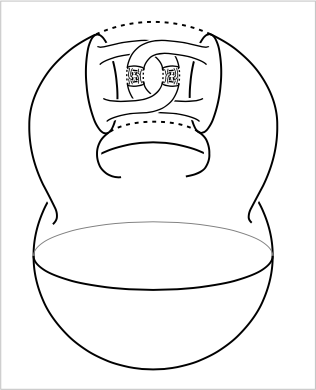
\includegraphics[width=40mm]{Hatcher-HornedSphere.png}
\caption{copied from Hatcher (171) \label{overflow}}
\end{figure}
It turns out that $X \cong D^3$, so that $\partial{X} \cong S^2$. (Yet, the exterior of $X$ is not simply connected, unlike the exterior of $D^3$ in $\R^3$.)
\end{enumerate}
\end{exmp}


The following are types of spaces that we will care about.
\begin{enumerate}
\item \underline{Manifolds}.
\begin{definition}
A space $X$ is \textit{homogeneous} if for any $x,y \in X$ with $x\ne y$, there is some homeomorphism $f: X \to X$ such that $f(x)= y$ and $f(y) =x$.
\end{definition}
\begin{prop}
Any connected manifold is homogenous. 
\end{prop}
With respect to connected manifolds, we may thus restrict our attention to questions of global topology.
\item \underline{Algebraic varieties over $\R$ or $\C$}.
\begin{exmp}
Consider the affine variety $Z(xy) =\left\{(x, y) \in \R^2 : x=0 \lor y=0\right\}$. This is not homogenous, because of the singularity $(0,0)$.  
\end{exmp}
\item \underline{The Cantor set $\mathcal{C}$}. This is the unique homeomorphism class of spaces that are compact, metrizable, and totally disconnected. 
\begin{exmp}
Given a prime $p$, complete $\Q$ endowed with the $p$-adic metric $\lvert{\cdot}\rvert_p$ to obtain the $p$-adic numbers $\Q_p$. Then the ring of $p$-adic integers $\mathcal{O}_p \subset \Q_p$ is the Cantor set.
\end{exmp}
\item \underline{CW-complexes} (developed by J. H. C. Whitehead).\footnote{$ \underbrace{\text{C}}_{\text{cell}}\underbrace{\text{W}}_{\text{weak}} $} 

Recall that an $n$-cell is a space homeomorphic to $\Int{D^n}$ where $D^n \coloneqq  \left\{x \in \R^n : \lvert{x}\rvert \leq 1\right\}$.

Start with a discrete set $X^0$, called a \textit{$0$-skeleton}. 

By induction, define the \textit{$n$-skeleton} as $$X^n = \faktor{X^{n-1} \coprod_{\alpha} D^n_{\alpha}}{\sim}$$ where $\varphi_{\alpha}: S^{n-1} \to X^{n-1}$ is an \textit{attaching map} and $x\sim \varphi_{\alpha}(x)$ for each $x\in \partial{D^n_{\alpha}}$. Then $$X^n = X^{n-1} \coprod_{\alpha} e^n_{\alpha}$$ where each $e^n_{\alpha}$ is an $n$-cell.

Set $X= \bigcup_{n} X^n$ and endow it with the \textit{weak topology}: $A$ is open in $X$ if and only if $A\cap X^n$ is open in $X^n$ for each $n$.
\begin{definition} $ $
\begin{enumerate}
\item If $X$ is a CW-complex, then the \textit{dimension of $X$} is the maximum dimension of cells of $X$.
\item If $X$ is a CW-complex consisting of only finitely many cells, then it is called a \textit{finite CW-complex}.
\end{enumerate}
\end{definition}
Each cell $e_{\alpha}^n$ has a \textit{characteristic map $\Phi_{\alpha} : D_{\alpha}^n \to X$} given by the composite $$D_{\alpha}^n \hookrightarrow X^{n-1} \coprod_{\alpha} D_{\alpha}^n \twoheadrightarrow X^n \hookrightarrow X.$$ This extends the attaching map $\varphi_{\alpha}$ and is a homeomorphism $\Int{D_{\alpha}^n} \to e_{\alpha}^n$.
\end{enumerate}


\begin{note}
If $X$ is a CW-complex, then any function $f: X \to Y$ is continuous if and only if $f\restriction_{X^n}$ is continuous for each $n\geq 0$.
\end{note}

\begin{exmp} The following are CW-complexes.
\begin{enumerate}
\item Any singleton $\{p\}$.
\item Any $n$-sphere $S^n$.

$S^0 = \{\pm 1\}$.

Construct $S^1$ by adding semi-circles (i.e., $1$-cells) above and below $S^0$.

Construct $S^2$ by adding hemispheres (i.e., $2$-cells) above and below $S^1$.
\item Any orientable surface of genus $g$. 

Consider the case where $g=1$. Draw the torus $S^1 \times S^1$ as
\[
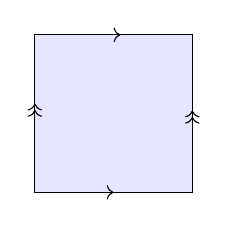
\begin{tikzpicture}[insert arrow/.style args={#1/#2}{postaction={decorate,
decoration={markings,mark=at position #1 with {\arrow{#2}}}}}]
 \draw[fill=blue!10,insert arrow/.list={0.125/>,0.37/>,0.38/>,0.625/<,0.87/<,0.88/<}] (0,0) -| ++ (2,2) -| cycle;
\end{tikzpicture}
\] The frame and interior are homeomorphic to the $1$-skeleton $S^1 \vee S^1$ and the $2$-cell $\Int{D^2}$, respectively.

Next, consider the case where $g=2$. Similarly, we can draw the two-holed torus as

\[
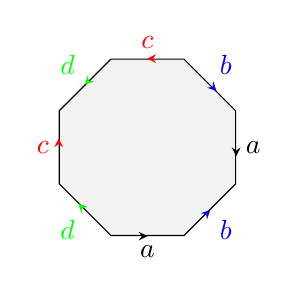
\begin{tikzpicture}


\node[fill=gray!10] (pol) [
  draw,
  minimum size=0.2\textwidth,
  regular polygon, regular polygon sides=8,
  ]{};
\foreach \x/\y/\i in {1/2/1} %\alpha's
  \path[red,auto=right, ->-]
    (pol.corner \x)--(pol.corner \y)
      node[red,midway]{$c$};
\foreach \x/\y/\i in {3/4/1} %inverse \alpha's
   \path[red,auto=right, -<-]
     (pol.corner \x)--(pol.corner \y)
     node[red,midway]{$c$};
\foreach \x/\y/\i in {2/3/1} %\beta's
  \path[green,auto=right, ->-]
    (pol.corner \x)--(pol.corner \y)
      node[green,midway]{$d$};
\foreach \x/\y/\i in {4/5/1} %inverse \beta's
   \path[green,auto=right, -<-]
     (pol.corner \x)--(pol.corner \y)
     node[green,midway]{$d$};
      \foreach \x/\y/\i in {5/6/1} %inverse \beta's
   \path[auto=right, ->-]
     (pol.corner \x)--(pol.corner \y)
     node[midway]{$a$};
      \foreach \x/\y/\i in {6/7/1} %inverse \beta's
   \path[blue,auto=right, ->-]
     (pol.corner \x)--(pol.corner \y)
     node[blue,midway]{$b$};
      \foreach \x/\y/\i in {7/8/1} %inverse \beta's
   \path[auto=right, -<-]
     (pol.corner \x)--(pol.corner \y)
     node[midway]{$a$};
 \foreach \x/\y/\i in {8/1/1} %inverse \beta's
   \path[blue,auto=right, -<-]
     (pol.corner \x)--(pol.corner \y)
     node[blue,midway]{$b$};

 
\end{tikzpicture}
\]

This is clearly a two-dimensional CW-complex.
\end{enumerate}
\end{exmp}

\begin{prop}
Every manifold has a CW-structure. 
\end{prop}

\begin{exmp} $ $
\begin{enumerate}
\item The Cantor set does not have a CW-structure, because it is totally disconnected.
\item Consider the subspace of $\R^2$ known as the Hawaiian earring. 
\[
 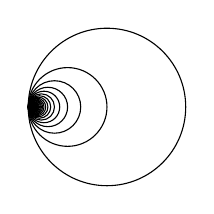
\begin{tikzpicture} 
  \foreach \n in {1,...,140} 
   \draw (1/\n,0) circle (1/\n);
 \end{tikzpicture}
\] If this had a CW-structure, then the sequence $\left(\frac{2}{n}, 0\right)_{n\in \N}$ would not converge to $(0, 0)$, which is absurd.
\end{enumerate}
\end{exmp}

\bigskip

At this point, let us review a some basic concepts from homotopy theory.

\begin{definition}
Let $f,g: X \to Y$ be maps. A \textit{homotopy from $f$ to $g$} is a map $H: X \times I \to Y$ such that $H(x,0) = f(x)$ and $H(x,1) = g(x)$ for each $x\in X$. We say that $f$ is \textit{homotopic to $g$}, written as $f\simeq g$.
\end{definition}

\begin{remark}
From now on, assume that every topological space is Hausdorff. 
\end{remark}

\begin{definition}
Let $A\subset X$ be a subspace. A \textit{homotopy between $f$ and $g$ relative to $A$} is a homotopy $F$ between $f$ and $g$ such that if $t\in [0,1]$, then $F(x, t) = f(x) = g(x)$ for each $x\in A$.
\end{definition}

\begin{exmp}
Let $X\coloneqq  D^2 \setminus \{0\}$. Define $f: X \to X$ by $f(r, \theta) = (r, \theta)$ and $g: X \to X$ by $g(r, \theta) = (1, \theta)$. Then the map $F: X \times I \to X$ given by  $F((r, \theta), t)=  \left(t+ (1-t)r, \theta\right)$ is a homotopy between $f$ and $g$ relative to $S^1\subset X$.
\end{exmp}

\begin{definition}
A \textit{deformation retraction of $X$ onto $A\subset X$} is a map $F: X \times I \to X$ such that 
\begin{enumerate}[label=(\roman*)]
\item $F(x, 0) = x$ for each $x\in X$, 
\item $F(a, 1) = a$ for each $a\in A$, and 
\item $F(x, 1) \in A$ for each $x\in X$.
\end{enumerate}
\end{definition}

\begin{exmp}
The solid torus $S^1 \times D^2$ deformation retracts onto $S^1$, as does the solid coffee mug. In fact, we have a homeomorphism transforming the hollow coffee mug to the torus:

\begin{figure}[H]
\centering
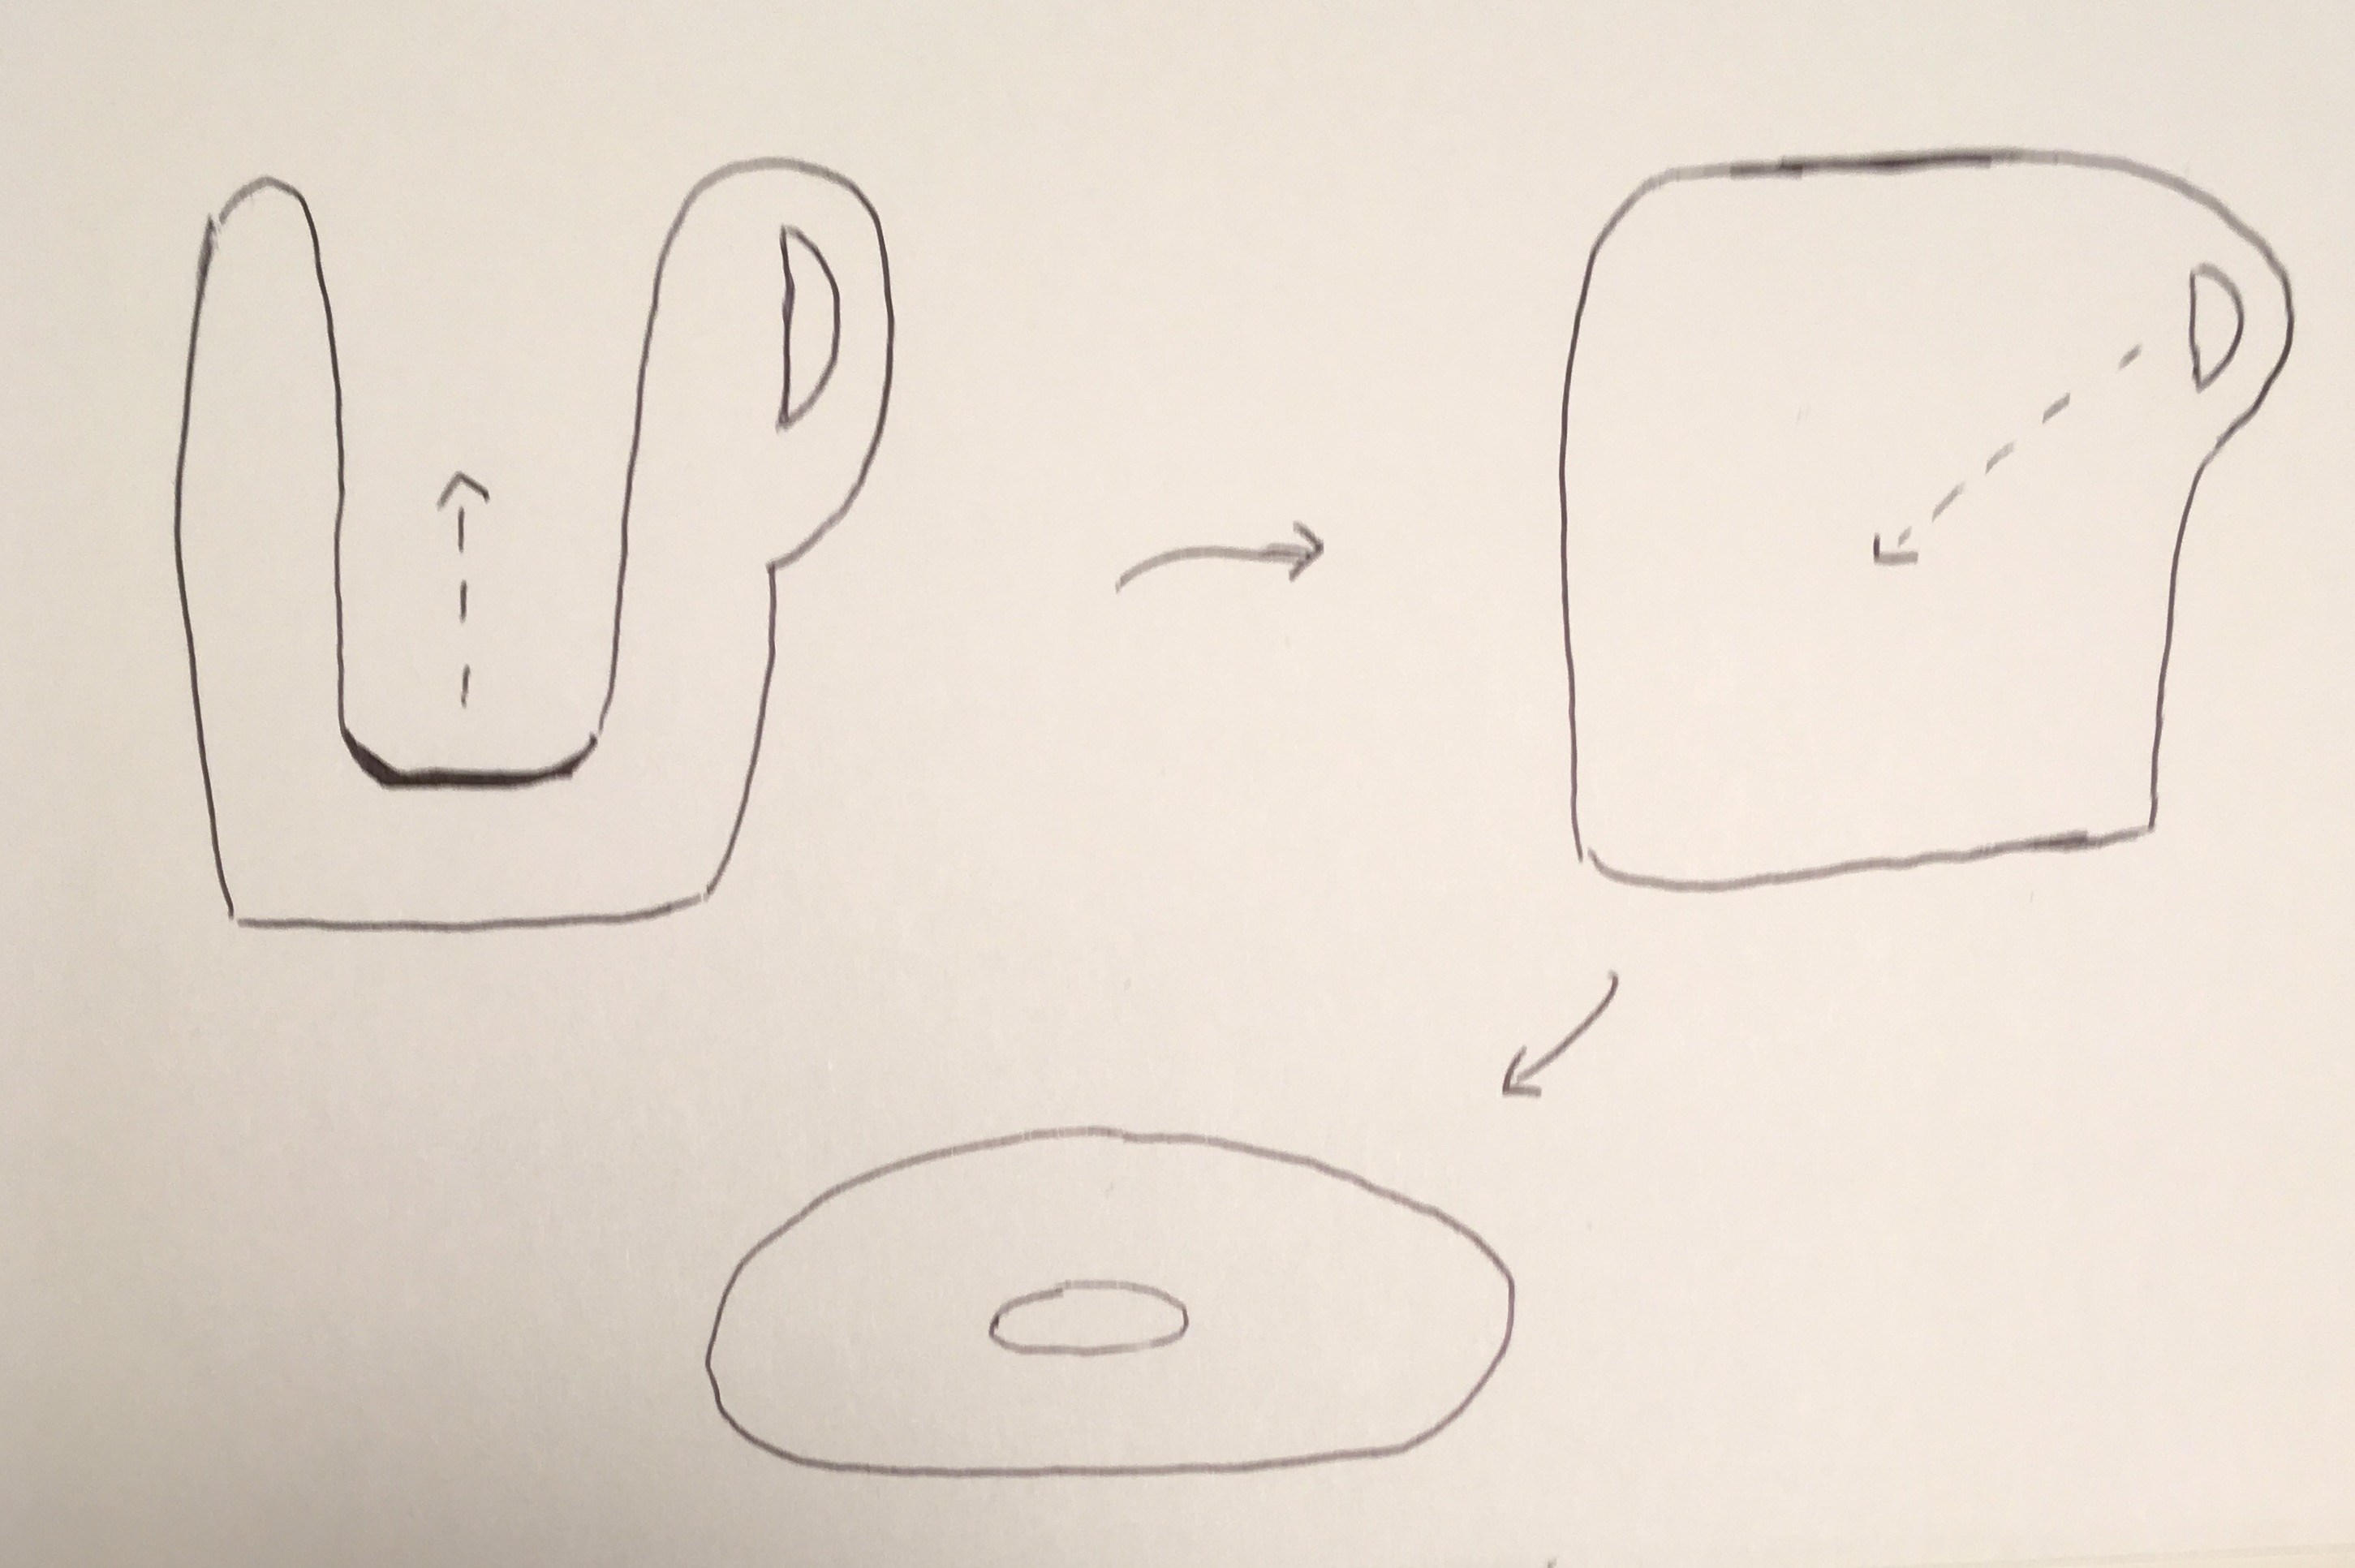
\includegraphics[width=55mm]{mug.jpg}
\end{figure}
\end{exmp}

\begin{definition}
Two spaces $X$ and $Y$ are \textit{homotopy equivalent $(\simeq)$} if there are maps $f: X\to Y$ and $g: Y \to X$ such that $f\circ g \simeq \mathbb{1}_Y$ and $g\circ f \simeq \mathbb{1}_X$.
\end{definition}

\begin{definition}
A space is \textit{contractible} if it is homotopy equivalent to $\{\ast \}$.
\end{definition}

Equivalently, a space $X$ is contractible if $\id_X$ is \textit{nullhomotopic}, i.e., homotopic to the constant map at $c$ for some $c\in X$.

\begin{lemma}
Homotopy equivalence of maps is an equivalence relation.
\end{lemma}
\begin{proof}
Both reflexivity and symmetry are obvious. To check transitivity, suppose that $F : f \simeq g$ and $G: g\simeq h$. Define $$H(x,t) = \begin{cases}
F(x, 2t) & 0 \leq t \leq \frac{1}{2}
\\ G(x, 2t-1) & \frac{1}{2} \leq t \leq 1
\end{cases}.$$ Then $H : f \simeq h$, as required. 
\end{proof}

\begin{prop}
Homotopy equivalence of spaces is an equivalence relation.
\end{prop}
\begin{proof}
Recall the category $h\mathbf{Top}$ with spaces as objects and homotopy classes of maps $X \to Y$ as morphisms. Then two objects are isomorphic if and only if they are homotopy equivalent. But it's clear that any categorical isomorphism is an equivalence relation.  
\end{proof}

\subsection{Lecture 2}

\begin{exmp}[Projective space]
\begin{enumerate}
\item Recall that $\RP^n \cong \faktor{S^n}{\alpha}$ where $\alpha$ denotes the antipodal map. Thus, $\RP^n \cong \faktor{D^n}{\sim}$ where $x\sim y$ if $x,y\in \partial{D^n}$ and $x={-y}$. This implies that $\RP^n \cong \RP^{n-1} \cup_{\pi} D^n$ where $\pi : \partial{D^n} = S^{n-1} \to \RP^{n-1}$ denotes projection. By induction, we have that $$\RP^n \cong e^0 \cup e^1 \cup \cdots \cup e^n.$$
\item Recall that $$\CP^n = \left\{\underbrace{[z_0 : \cdots : z_n]}_{\text{homogeneous coordinates}} : z_i \in \C, \ (z_0, \ldots, z_n) \ne 0\right\}.$$ Note that $\CP^n \cong \faktor{S^{2n+1}}{U(1)}$.
We see that $S^{2n+1} = \left\{(w, \sqrt{1-\lvert{w}\rvert^2}) \in \C^n \times \C : \lvert{w}\rvert \leq 1\right\}$. When $(w,z) \in S^{2n+1}$ has $z\ne 0$, then $(w,z) \sim (x', y')$ for some unique $(x', y')\in D^{2n}$. Otherwise, $(w,z) \in S^{2n-1}$. This shows that $\CP^n \cong \CP^{n-1} \cup_{\pi} D^{2n}$ where $\pi : S^{2n-1} \to \CP^{n-1}$ denotes projection.  By induction, we get $$\CP^n \cong e^0 \cup e^2 \cup \cdots \cup e^{2n}.$$
\end{enumerate}
\end{exmp}

\begin{definition}
A closed subspace $A$ of a CW-complex $X$ is a \textit{subcomplex} if $A$ equals some union of cells of $X$. In this case, the pair $(X, A)$ is called a \textit{CW pair}.
\end{definition}

\begin{note} Let $X$ and $Y$ be pointed CW-complexes. Let $A\subset X$ be a subcomplex.
\begin{enumerate}
\item $X\coprod Y$ is a CW-complex.
\item $X \vee Y$ is a CW-complex.
\item $X\times Y$ is a CW-complex.

 The topology of $X \times Y$ as a CW-complex, however, may be finer than $X\times Y$ equipped with the product topology. 

Moreover, an uncountable product of CW-complexes under the product topology need \emph{not} be a CW-complex.


\item $\faktor{X}{A}$ is a CW-complex whose cells are precisely those of $X\setminus A$ together with the $0$-cell $\pi(A)$ and attaching maps are precisely $\pi_{n-1} \circ \varphi_{\alpha}$ where $\pi_{n-1} : X^{n-1} \to \faktor{X^{n-1}}{A^{n-1}}$ denotes projection and $\varphi_{\alpha} :S^{n-1} \to X^{n-1}$ is an attaching map. 
\begin{exmp}
$\faktor{D^n}{S^{n-1}} \cong S^2$ for any $n\geq 1$.
\end{exmp}
\end{enumerate}
\end{note}

\begin{definition}
Given any space $X$, define the \textit{cone of $X$} as $$C(X) = \faktor{X\times I}{(x,1) \sim (y,1)}.   $$
\end{definition}
\begin{lemma}
$C(X)$ is contractible.
\end{lemma}
\begin{proof}
Define $H((x,t), s) = \begin{cases} \left(x, (1-s)t\right) & t\ne 1 \\ (x,1) & t=1
\end{cases}.$
\end{proof}

\begin{definition}
Given any space $X$, the \textit{suspension of $X$} is $$S(X) \equiv\faktor{X\times I}{\sim}$$ where $(x,0) \sim (x', 0)$ and $(x,1) \sim (x', 1)$. 
\end{definition}
\begin{exmp}
$S(S^n) = S^{n+1}.$
\end{exmp}

\begin{prop}
Both $C(-)$ and $S(-)$ preserve the property of being a CW-complex (``CW-hood'').
\end{prop}

\begin{definition}
Let $f: X \to Y$ be a map of spaces. Define the \textit{mapping cylinder of $f$} as $$\cyl(f) = \faktor{(X\times I) \coprod Y}{(x, 1) \sim f(x)}.$$
\end{definition}
\begin{note}
$\cyl(-)$ need \emph{not} preserve CW-hood.
\end{note}
\begin{lemma}
$\cyl(f) \simeq Y$.
\end{lemma}
\begin{proof}
Define $$f: \cyl(f) \to Y, \quad (x,t) \mapsto f(x) \quad y \mapsto y$$ and
$$ g: Y \to \cyl(f), \quad y \mapsto y . $$ We see that $f\circ g = \mathbb{1}_Y$.
\begin{exercise}
Prove that $g\circ f \simeq \mathbb{1}_{\cyl(f)}$.
\end{exercise}
\end{proof}

\begin{exmp} $ $
\begin{enumerate}
\item Consider the following subspace of $\R^2$, called the comb space.
\[
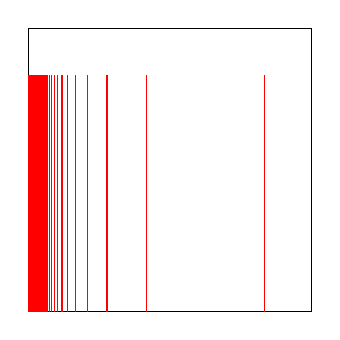
\begin{tikzpicture}[scale=3]
  \draw (0,0)--(1.2,0)--(1.2,1.2)--(0,1.2)--cycle;
  \draw[color=red, thin] (1,0)--(1,1);
  \draw[color=red, thin]  (1/2,0)--(1/2,1);
  \draw[color=red, thin]  (1/3,0)--(1/3,1);
  \foreach \x in {4, ..., 20}
   \draw[color=red, thin]  (1/\x,0)--(1/\x,1);
  \fill[color=red]  (1/20,0)--(1/20,1)--(0,1)--(0,0)--cycle;
\end{tikzpicture}
\] This deformation retracts onto $(0,0)$ but not onto $(0,1)$. 
\item Let $X$ denote the comb space. Rotate $X$ clockwise by $180$ degrees to obtain the space $A$. Set $Y = X \cup A$ and note that $A$ is closed in $Y$. Then both $A$ and $\faktor{Y}{A}$ are contractible, but $Y$ is not.
\end{enumerate}
\end{exmp}

\begin{definition}
Let the pair $(X, A)$ consist of a space $X$ and a subspace $A \subset X$. We say that $(X, A)$ has the \textit{homotopy extension property (HEP)} if we can fill the commutative diagram
\[
\begin{tikzcd}
X\times \{0\} \arrow[rr, hook] \arrow[rd, "f"] &  & X\times I \arrow[ld, dashed] \\
 & Y &  \\
A\times \{0\} \arrow[uu, hook] \arrow[rr, hook] &  & A\times I \arrow[uu, hook] \arrow[lu, "H"']
\end{tikzcd}
\] of spaces where $H$ is a given homotopy from $f \restriction_{A}$ to another map. The inclusion $\iota : A \to X$ is called a \textit{cofibration} if $(X, A)$ satisfies HEP.
\end{definition}

\subsection{Lecture 3}

\begin{lemma}
The pair $(X, A)$ has HEP if and only if $A\times I \cup X \times \{0\}$ is a retract of $X\times I$.
\end{lemma}
\begin{proof} $ $

\smallskip

($\Longrightarrow$) We have a commutative diagram
\[
\begin{tikzcd}
A\times \{0\} \arrow[dd] \arrow[rr] &  & A\times I \arrow[ld] \arrow[dd] \\
 & A\times I \cup X \times \{0\} &  \\
X\times \{0\} \arrow[ru] \arrow[rr] &  & X\times I \arrow[lu, "\varphi"', dashed]
\end{tikzcd}
.\] Then $\varphi$ is a retraction, as desired. 

\medskip

($\Longleftarrow$) By hypothesis, there is some retraction $r: X\times I \to X\times \{0\} \cup A \times I$. This enables us to fill the diagram
\[
\begin{tikzcd}
A\times \{0\} \arrow[dd] \arrow[rr] &  & A\times I \arrow[ld, "H"'] \arrow[rddd] &  \\
 & Y &  &  \\
X\times \{0\} \arrow[ru, "f"] \arrow[rrrd] &  & A\times I \cup X \times \{0\} \arrow[lu, "H \cup f"', dashed] &  \\
 &  &  & X\times I \arrow[lu, "r"']
\end{tikzcd}
.\] If $A$ is closed then $H\cup f$ is certainly continuous. If $A$ is not closed, then our argument needs to be more careful. 
\end{proof}

\begin{exmp}\label{ex12} $ $
\begin{enumerate}[label=(\alph*)]
\item $S^{n-1} \hookrightarrow D^n$ is a cofibration. 
\begin{proof}
We see that $\left(S^{n-1} \times I\right) \cup \left(D^n \times \{0\}\right)$ is a retract of $D^n \times I$ by the following radial projection from the point $(0,2)$.
\begin{figure}[H]
\centering
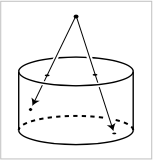
\includegraphics[width=30mm]{Hatcher-radial_proj.png}
\caption{copied from Hatcher (15) \label{overflow}}
\end{figure} In fact, setting $r_t(x) = tr(x) +(1-t)x$ for each $t\in I$ defines a deformation retraction $r$ of $D^n \times I$ onto $S^{n-1} \times I \cup D^n \times \{0\}$.
\end{proof}
\item Let $A= \left\{0, 1, \frac{1}{2}, \frac{1}{3}, \frac{1}{4}, \ldots\right\}$. Then $A \hookrightarrow I$ is \emph{not} a cofibration.
\begin{proof}
Suppose, toward a contradiction, that there is some retraction $r: I \times I \to A \times I \cup I \times \{0\}$. For each $n\geq 1$, the set $c_n \coloneqq  \left[\left(\frac{1}{n+1}, 1), (\frac{1}{n}, 1\right)\right]$ is connected, so that $r(c_n)$ is connected as well. Thus, there exists $(x_n, 1) \in c_n$ such that $r(x_n, 1) = (x_n ,0)$. But then $(x_n, 1) \to (0, 1)$ whereas $r(x_n, 1) \to (0, 0)$. As $r(0,1) = (0,1)$, this contradicts the continuity of $r$. 
\end{proof}
\item Let $f: B \to A$ be a map. Then $\left(\cyl(f), B \times \{0\}\right)$ satisfies HEP.
\end{enumerate}
\end{exmp}

\begin{lemma}
Any CW pair $(X,A)$ satisfies HEP.
\end{lemma}
\begin{proof}
Notice that $X^n \times I$ is obtained from $\left(X^n \times \{0\}\right) \cup \left(\left(X^{n-1} \cup A^n\right) \times I\right)$ by attaching a certain number of copies of $D^n \times I$ along $D^n \times \{0\} \cup S^{n-1} \times I$. Recall the deformation retraction $r$ from  \cref{ex12}(b). Thus, we obtain a deformation retraction $r_n$ of $X^n \times I$ onto $X^n \times \{0\} \cup (X^{n-1} \cup A^n) \times I$.

Define $U_n = X\times \{0\} \cup (X^n \cup A) \times I$ for each $n\geq -1$ with $X^{n-1} = \emptyset$. Note that $U_n = (X^n \times I) \cup U_{-1}$. Extend each $r_n$ to the homotopy $\hat{r}_n : U_n \times I \to U_n$ given by setting $\hat{r}_n(x) = x$ for each $x\in U_{-1}$. This is continuous since $A$ is closed and $(X^n \times I) \cap U_{-1} = X^n \times \{0\} \cup A^n \times I \subset X^n \times \{0\} \cup (X^{n-1} \cup A^n) \times I$. Then each $\hat{r}_n$ is a deformation retraction of $U_n$ onto $U_{n-1}$.  Perform $\hat{r}_n$ during the $t$-interval $\left[\frac{1}{2^{n+1}}, \frac{1}{2^n}\right]$.  The infinite sequential concatenation $R$ of the $\hat{r}_n$ is continuous at $t=0$ when restricted to each $X^n \times I^2$  and is thus continuous on $\bigcup_n U_n = X \times I^2$. Therefore, $R$ is a deformation retraction of $X\times I$ onto $U_{-1} = X\times \{0\} \cup A\times I$.
\end{proof}

\begin{definition}
Let $X$ be a space. Define $\pi_0(X) = \faktor{X}{\sim} $ where $x\sim y$ if $\exists \varphi: I \to X$ such that $\varphi(0)=x$ and $\varphi(1) = y$.
\end{definition}

This means that $\pi_0(X)$ is precisely the set of path components of $X$.

\begin{definition}
Let $\gamma, \hat{\gamma}: I \to X$ be paths in $X$ such that $\gamma(0) = \hat{\gamma}(0)$ and $\gamma(1) = \hat{\gamma}(1)$.  A \textit{path homotopy from $\gamma$ to $\hat{\gamma}$} is a homotopy $H: I \times I \to X$ such that $H(0,s) = \gamma(0)$ and $H(1,s) = \gamma(1)$ for each $s\in I$. In this case, we write $\gamma \simeq_p \hat{\gamma}$.
\end{definition}

\begin{prop} $ $
\begin{enumerate}
\item If $\gamma_0 \simeq_p \gamma_1$ and $\eta_0 \simeq_p \eta_1$, then $\gamma_0 \ast \eta_0 \simeq_p \gamma_1 \ast \eta_1$.
\item $(\gamma_0 \ast \gamma_1)\ast \gamma_2 \simeq_p \gamma_0 \ast (\gamma_1 \ast \gamma_2)$.
\item Any map $f: X \to Y$ induces a map $f_{\ast} : \pi_0(X) \to \pi_0(Y)$. If $\gamma_0 \simeq_p \gamma_1$, then $f\circ \gamma_0 \simeq_p f\circ \gamma_1$.
\item For any path $\gamma : I \to X$, the path $\eta(t) \coloneqq  \gamma(1-t)$ satisfies $\eta \ast \gamma \simeq_p c_{\gamma(1)}$ and $\gamma \ast \eta \simeq_p c_{\eta(1)}$ where $c_x$ denotes the constant path at the point $x\in X$.
\end{enumerate}
\end{prop}


\smallskip

Define the \textit{fundamental groupoid of a space $X$} as the category $\Pi_1(X)$ with $\ob(\Pi_1(X)) = X$ and $\Hom_{\Pi_1(X)}(x,y) = \left\{[\gamma]_{\simeq_p} \mid \gamma \text{ is a path from }x \text{ to }y\right\}$. We make concatenation of paths the composition of morphisms. 



This is, in fact, a groupoid in the sense of category theory.


\begin{definition}
Given $x_0 \in X$, define the \textit{fundamental group of the pointed space $\left(X, x_0\right)$} as $$\pi_1\left(X, x_0\right) = \Hom_{\Pi_1(X)}(x_0,x_0) .$$ 
\end{definition}

This means that $\pi_1\left(X, x_0\right) \equiv  \faktor{\left\{\gamma : S^1 \to X \mid \gamma(1,0) =x_0\right\}}{\simeq (\rel \ (1,0))}$.

\begin{remark}
Any map $f: X \to Y$ induces a functor $f_{\ast} : \Pi_1(X) \to \Pi_1(Y)$ that restricts to a homomorphism $f_{\ast} : \pi_1\left(X, x_0\right) \to \pi_1(Y, f(x_0))$.
\end{remark}

\begin{prop}
If there is some path $p$ from $x$ to $y$ in $X$, then $\pi_1(X, x) \cong \pi_1(X, y)$.
\end{prop}
\begin{proof}
Define $\varphi_p : \pi_1(X, x) \to \pi_1(X, y)$ by $\gamma \mapsto p^{-1} \gamma p$. This is an isomorphism. 
\end{proof}

\begin{theorem}
If $n\geq 2$, then $\pi_1(S^n, x) =0$, i.e., $S^n$ is \textit{simply connected}.
\end{theorem}
\begin{proof}
Note that if $\eta : I \to S^n$ satisfies $\im{\eta} = S^n \setminus \{p\}$ for some $p\in S^n$, then $\eta \simeq_p c_x$ since $S^n \setminus \{p\} \cong \R^n$. Thus, it suffices to prove the following lemma.
\begin{lemma}
Every path $\gamma$ in $S^n$ is path-homotopic to some path $\eta$ in $S^n$ such that $\im{\eta} \ne S^n$.
\end{lemma}
\begin{proof}
Write $\gamma(t) = \left(\gamma_0(t), \gamma_1(t), \ldots, \gamma_n(t)\right)$. The Weierstrass approximation theorem implies that we can approximate each $\gamma_i$ by some smooth function. Hence we may find some smooth map $\tilde{\gamma}$ such that $$\lvert{\gamma(t) - \tilde{\gamma}(t)}\rvert <\epsilon$$ for each $t\in I$. Now, there is some smooth retraction $r: D^{n+1}\setminus \{0\} \to S^n$. Define $H : I \times I \to S^n$ by $$(t, s) \mapsto r(s\tilde{\gamma}(t) + (1-s)\gamma(t)).$$ This is a homotopy $\gamma \simeq_p r\circ \tilde{\gamma}$. But $r\circ \tilde{\gamma} : I \to S^n$ is smooth and $n>1$. By Sard's theorem, it follows that $\im(r\circ \tilde{\gamma})$ has measure zero in $S^n$. Thus, $r\circ \tilde{\gamma}$ is not surjective, as desired. 
\end{proof}
\end{proof}

\subsection{Lecture 4}

\begin{theorem}
If the pair $(X, A)$ has HEP and $A$ is contractible, then the natural projection $X \twoheadrightarrow \faktor{X}{A}$ is a homotopy equivalence. 
\end{theorem}
\begin{proof}
There is some contraction $H: A \times I\to X$ of $A$ onto, say, $a_0$. We can find some map $\widetilde{H}$ such that 
\[
\begin{tikzcd}
A\times \{0\} \arrow[rr, hook] \arrow[dd, hook] &  & A\times I \arrow[dd, hook] \arrow[ld, "H"'] \\
 & X &  \\
X\times \{0\} \arrow[rr, hook] \arrow[ru, hook] &  & X\times I \arrow[lu, "\widetilde{H}"', dashed]
\end{tikzcd}
\] commutes. Then $\widetilde{H}_0 = \1_X$, and $\widetilde{H}_t(A) \subset A$ for each $t\in I$. By the universal property of quotient spaces, we get some $\bar{H}_t$ such that
\[
\begin{tikzcd}
X \arrow[d, two heads] \arrow[r, "\widetilde{H}_t"] & X \arrow[d, two heads] \\
\faktor{X}{A} \arrow[r, "\bar{H}_t"', dashed] & \faktor{X}{A}
\end{tikzcd}
\] commutes for each $t$. Since $\widetilde{H}_1(a) = a_0$ for each $a\in A$, it follows that 
\[
\begin{tikzcd}
X \arrow[d, two heads] \arrow[r, "\widetilde{H}_1"] & X \arrow[d, two heads] \\
\faktor{X}{A} \arrow[r, "\bar{H}_1"'] \arrow[ru, "p", dashed] & \faktor{X}{A}
\end{tikzcd}
\] commutes as well for some map $p$. If $q$ denotes the natural projection, then $$q\circ p(\bar{x}) = q \circ p \circ q({x}) = \bar{H}_1 \circ q({x}) = \bar{H}_1(\bar{x}).$$ Then $p$ is homotopy inverse to $q$.
\end{proof}

\begin{prop}
If $X$ is contractible, then $\pi_1\left(X, x_0\right) = 0$.
\end{prop}
\begin{proof}
By hypothesis, there is some contraction $F: X \times I \to X$ of $X$ onto, say, the point $x_0$. Let $\gamma : I \to X$ be a loop at $x_0$. This yields a homotopy $G: c_{x_0} \simeq \gamma$ where each $G_t$ is a loop in $X$.
\begin{lemma}\label{chom}
Let $F: I \times I \to X$ be  any homotopy. Let $\gamma \coloneqq  F\restriction_{\{0\} \times I}$, $\beta \coloneqq  F\restriction_{I \times \{1\}}$, $\delta \coloneqq  F\restriction_{\{1\} \times I}$, and $\alpha \coloneqq F \restriction_{I \times \{0\}}$. Then $\beta \simeq_p \gamma^{-1} \ast \alpha \ast \delta$. 
\end{lemma}
\begin{proof} Write $\gamma(1) = x_0$ and $\delta(1) = x_1$. Define the path homotopies 
\begin{align*}
G(s,t) &\equiv \begin{cases} x_0 & s\leq t \\ \gamma(1 + t-s) & s \geq t   \end{cases}
\\ H(s,t) & \equiv \begin{cases}  x_1 & 1-s \leq t \\ \delta(s+t) & 1-s \geq t  \end{cases} .
\end{align*} Then $G: c_{x_0} \simeq_p \gamma^{-1}$, and $H: c_{x_1} \simeq_p \delta$. Hence $$\beta \simeq_p c_{x_0} \ast \beta \ast c_{x_1} \simeq_p \gamma^{-1} \ast \alpha \ast \delta, $$ as desired. 
\end{proof}
 Since $\eta \coloneqq  G\restriction_{\{0\} \times I} = G \restriction_{\{1\} \times I}$, \cref{chom} implies that $c_{x_0} \simeq_p \eta^{-1} \ast c_{x_0} \ast \eta \simeq_p \gamma$. 
\end{proof}


\section{Covering spaces} 

\begin{definition}
We say that a map $p: Y \to X$ is a \textit{covering projection} if for each $x\in X$, there exists a neighborhood $U\ni x$ together with a discrete space $S$ and a homeomorphism $h_U : p^{-1}(U) \overset{\cong}{\longrightarrow} U \times S$  such that 
\[
\begin{tikzcd}
p^{-1}(U) \arrow[rd, "p"'] \arrow[r, "h_U"] & U \times S \arrow[d, "\pi_1"] \\
 & U
\end{tikzcd}
\] commutes. In this case, we say that $Y$ is a \textit{covering space of $X$}.
\end{definition}

\begin{term} $ $
\begin{enumerate}
\item 
We call a triple of the form $\left(X \times S, X, \pi_1\right)$ a \textit{trivial covering space}.
\item  If there is some $n\in \N$ such that every $S$ has cardinality $n$, then $p$ is called an \textit{$n$-fold cover of $X$}.
\end{enumerate}
\end{term}

\begin{prop}
If $p: Y \to X$ is a covering projection, then $Y$ is a manifold if and only if $X$ is a manifold. 
\end{prop}

\begin{exmp} $ $
\begin{enumerate}
\item $p : \R \to S^1$ given by $x \mapsto e^{2\pi ix}$.
\item $p: S^1\subset \C^{\times} \to S^1$ given by $z \mapsto z^n$.
\item $p: S^n \to \RP^n$ given as the quotient map is a $2$-fold cover of $\RP^n$.
\end{enumerate}
\end{exmp}

\smallskip

Let $X$ be a space and $\Gamma$ be a discrete topological group. 
\begin{definition}
A \textit{group action on a space $X$} is an injective group homomorphism $G \to \homeo(X)$.
\end{definition}
Let $\Gamma$ act on the space $Y$ such that for every $y\in Y$, there is some open set $U\ni y$ such that $g\cdot U \cap U =\emptyset$ when $g\ne e$. We call such a group action \textit{a covering space action} or \textit{properly discontinuous}. In particular, this action is free.  Proposition 1.40(a) (Hatcher) states that $Y \twoheadrightarrow \faktor{Y}{\Gamma}$ is a covering projection.

\begin{remark}
If $Y$ is simply connected, then $\pi_1 \left(\faktor{Y}{\Gamma} , y_0 \right) \cong \Gamma$.
\end{remark}

Let $\alpha \in \R\setminus \Q$. We have that $S^1 \cong \faktor{\R}{x\sim x+1} \cong \faktor{\R}{\Z}$. Let $\Z$ act on $S^1$ by $n\cdot [x] = [x + n \alpha]$. But note that for any $x\in S^1$, the orbit of $x$ is dense in $S^1$ since $\alpha$ is irrational. Thus, $\faktor{S^1}{\Z}$ has the indiscrete topology, and $S^1 \twoheadrightarrow \faktor{S^1}{\Z}$ is \emph{not} a covering projection.


\begin{exmp} The following, however, are covering projections.
\begin{enumerate}
\item $\R^2 \twoheadrightarrow \faktor{\R^2}{\Z^2} \cong S^1 \times S^1$.
\item $\SL_2(\R) \twoheadrightarrow \faktor{\SL_2(\R)}{\SL_2(\Z)}$.
\item Set $G = \left \{ \begin{bmatrix} 1 & x & z \\ 0 & 1 & y \\ 0 & 0 & 1 \end{bmatrix}  \mid x,y,z \in \R \right \}$ and $\Gamma = \left \{ \begin{bmatrix} 1 & a & c \\  & 1 & b \\  &  & 1 \end{bmatrix} \mid a,b,c \in \R \right \}$. Then $\Gamma$ is a discrete subgroup of $G$, and $G \twoheadrightarrow \faktor{G}{\Gamma}$ is a covering projection. We call $\faktor{G}{\Gamma}$ an \textit{Iwasawa manifold}.
Since $G$ is simply connected, we also have that $\pi_1 \left(\faktor{G}{\Gamma} \right) \cong \Gamma$.
\end{enumerate}
\end{exmp}

\begin{exercise}
Prove that $\pi_1(X \times Y, (x_0, y_0)) \cong \pi_1\left(X, x_0\right) \times \pi_1\left(Y, y_0\right)$.
\end{exercise}

\begin{lemma}
Let $F : Z \times I \to X$ be any map and $p: Y \to X$ be a covering projection. Suppose that there is some $\widetilde{F}_0 : Z \times \{0\} \to Y$ such that $p \circ \widetilde{F}_0 = F_0$. Then there exists a unique map $\widetilde{F} : Z \times I \to Y$ such that $p \circ \widetilde{F} = F$ and $\widetilde{F} \restriction_{Z\times \{0\}} = \widetilde{F}_0$.
\end{lemma}

\begin{corollary}[Path lifting property]\label{cor1} $ $
\begin{enumerate}
\item If $\gamma : I \to X$ is a path and $y_0 \in Y$ with $p(y_0) = \gamma(0)$, then there exists a unique $\tilde{\gamma} : I \to Y$ such that $\tilde{\gamma}(0) = y_0$ and $p \circ \tilde{\gamma} = \gamma$.
\item Let $\gamma_0, \gamma_1$ be two paths in $X$ and let $H : \gamma_0 \simeq_p \gamma_1$. Let $\tilde{\gamma}_0$ and $\tilde{\gamma}_1$ be respective lifts such that $\tilde{\gamma}_0 (0) = \tilde{\gamma}_1(0)$. Then there exists a unique $\widetilde{H} : \tilde{\gamma}_0 \simeq_p \tilde{\gamma}_1$ such that $p \circ \widetilde{H} = H$.
\end{enumerate}
\end{corollary}
\begin{proof} $ $
\begin{enumerate}
\item Let $Z = \ast$
\item Let $Z = I$.
\end{enumerate}
\end{proof}

\begin{theorem}
$\pi_1(S^1, 1) \cong \Z$.
\end{theorem}
\begin{proof}
Let $\gamma$ be a path in $S^1$ based at $1$. We have a covering projection $p: \R \to S^1$ given by $t\mapsto e^{2\pi i t}$. By \cref{cor1}, there is some unique lift $\tilde{\gamma}$ of $\gamma$ such that $\tilde{\gamma}(0) = 0$ and $p \circ \tilde{\gamma} = \gamma$. Since $p^{-1}(1) = \Z$, \cref{cor1} gives a function $\psi: \pi_1(S^1, 1) \to \Z$ given by $[\gamma ] \mapsto \tilde{\gamma}(1)$. Since $\R$ is simply connected, we have that $\psi$ is bijective. It remains to verify that it's a homomorphism. Let $[f], [g] \in \pi_1(S^1, 1)$ and take their respective unique lifting $\tilde{f}$ and $\tilde{g}$. Write $n = \tilde{f}(1)$ and $m= \tilde{g}(1)$. Define the path $\tilde{\tilde{g}}(s) = n+ \tilde{g}(s)$ in $\R$, which begins at $n$. Since $p(n+x) = p(x)$ for every $x\in \R$, we see that $\tilde{\tilde{g}}$ lifts $g$. Then $\tilde{f} \ast \tilde{\tilde{g}}$ lifts $f \ast g$ and ends at the point $n+m$. Hence $\psi([f] \ast [g]) = n+m = \psi([f])  + \psi([g])$, as required. 
\end{proof}


\begin{corollary}
There is no retraction of $D^2$ onto $S^1$.
\end{corollary}
\begin{proof}
Suppose, toward a contradiction, that there is some retraction $r$. Then we get an induced sequence of group maps
\[
\begin{tikzcd}
{\pi_1(S^1, 1)} \arrow[r, "i_{\ast}"] & {\pi_1(D^2, 1)} \arrow[r, "r_{\ast}"] & {\pi_1(S^1, 1)}
\end{tikzcd}
.\] But $r_{\ast} \circ i_{\ast} = \left(r \circ i\right)_{\ast} = \left(\1_{S^1}\right)_{\ast} = \1_{\pi_1(S^1)}$. Thus, $r_{\ast}$ is surjective, which is impossible. 
\end{proof}

\begin{corollary}[Brouwer fixed point theorem in dimension 2]
If $\varphi : D^2 \to D^2$ is  any map, then $\varphi(x_0) = x_0$ for some $x_0 \in D^2$.
\end{corollary}
\begin{proof}
If not, then we may define a retraction $r$ of $D^2$ onto $S^1$ as follows. For each $x\in D^2$, set $r(x)$ equal to the point on the circle that intersects  the ray from $h(x)$ to $x$. 
\end{proof}

\subsection{Lecture 5}

To begin, let us prove a result that we've already used.

\begin{lemma}[Homotopy lifting property]\label{HLP}
Let $F : Z \times I \to X$ be any map and $p: Y \to X$ be a covering projection. Suppose that there is some $\widetilde{F}_0 : Z \times \{0\} \to Y$ such that $p \circ \widetilde{F}_0 = F_0$. Then there exists a unique map $\widetilde{F} : Z \times I \to Y$ such that $p \circ \widetilde{F} = F$ and $\widetilde{F} \restriction_{Z\times \{0\}} = \widetilde{F}_0$.
\end{lemma}
\begin{proof}
Let $z_0\in Z$.
\begin{claim} There exist a neighborhood $U_{z_0}\subset Z$ and a lift $\widetilde{F}$ of $F\restriction_{U_{z_0}\times I}$ such that $p \circ \widetilde{F} = F$ on $U_{z_0}\times I$.
\end{claim}
\begin{proof}
For any $(z_0, t) \in Z \times I$, note that $F(z_0, t)$ has some neighborhood $V_{z_0,t}$ such that $$p^{-1}(V_{z_0, t}) = \coprod_{\alpha} V_{z_0,t, \alpha}$$ with $p: V_{z_0, t, \alpha} \to V_{z_0, t}$ a homeomorphism. Thus, $F^{-1}(V_{z_0, t})$ contains some set of the form $\overbrace{U_{z_0, t}}^{\text{nbhd of } z_0} \times \left(a_t, b_t\right)$, so that $F(U_{z_0, t}  \times (a_t, b_t)) \subset V_{z_0, t} $. This makes $\left\{\left(a_t, b_t\right)\right\}_{t\in I}$ an open cover of $I$. As $I$ is compact, there is some $k\in \N$ such that $\{(a_{t_i}, b_{t_i})\}_{i=1, \ldots, k}$  cover $I$. Set $$U_{z_0} = \bigcap_{1\leq i \leq k} U_{z_0, t_i},$$ which must be  open and contain $z_0$. We obtain a sequence $$ 0= t_0 < t_1 < \cdots < t_n =1 $$ such that $F(U_{z_0} \times [t_i, t_{i+1}])$ is contained in an evenly covered set of $X$. 
Now, $\widetilde{F}_0 $ is contained in some unique sheet of $p^{-1}(U_{z_0, 0}) =\coprod_j \widetilde{U}_{z_0, 0, j} \subset Y$, say, $j_0$. Define $\widetilde{F} : U_{z_0} \times [0, t_1] \to \widetilde{U}_{z_0, 0, j_0}$ as the composite $p^{-1}_{j_0} \circ F \restriction_{U_{z_0} \times [0, t_1]}$ where $p_{j_0} : \widetilde{U}_{z_0, 0, j_0} \to U_{z_0, 0}$ is some homeomorphism.

\medskip

 Suppose that we have extended $\widetilde{F}$ to $U_{z_0} \times [0,t_i]$. We can use a similar argument to define an extension $\widetilde{F}$ on $U_{z_0} \times [t_i, t_{i+1}]$.  By induction, it follows that we can construct a lift $\tilde{F} : U_{z_0} \times I \to Y$ of $F$.
\end{proof}
 It remains to verify that such a lift is unique. For now, assume that $Z= \ast$. Suppose that $\widetilde{F}$ and $\widetilde{F}'$ are two lifts of $F: I \to X$ such that $\widetilde{F}(0) = \widetilde{F}'(0)$. Assume inductively that $\widetilde{F} = \widetilde{F}'$ on $[0,t_i]$. Since both $\widetilde{F}([t_i, t_{i+1}])$ and $\widetilde{F}'([t_i, t_{i+1}])$ are connected and $\widetilde{F}(t_i) = \widetilde{F}'(t_i)$, there is a single sheet over $U_{i-1}$ in which both $\widetilde{F}([t_i, t_{i+1}])$ and $\widetilde{F}'([t_i, t_{i+1}])$ are contained. Since $p$ is injective on this sheet and $p\circ \widetilde{F} = p \circ \widetilde{F}'$, it follows that $\widetilde{F} = \widetilde{F}'$ on $[t_i, t_{i+1}]$. We are done with our induction.


 As a result, the  lifts  $\{F \restriction_{U_{z} \times [0, t_1]}\}_{z\in Z}$ constructed above must agree with each other when $U_z \cap U_{z'} \ne \emptyset$. We may thus apply the gluing lemma to get a lift $\tilde{F} : Z \times I \to Y$ of $F$. This must be unique as it is unique when restricted to each segment $\{z\} \times I$.
\end{proof}

\begin{corollary}
Let $p: \left(Y, y_0\right) \to \left(X, x_0\right)$  be a covering projection. Then $p_{\ast} : \pi_1\left(Y, y_0\right) \to \pi_1\left(X, x_0\right)$ is injective. 
\end{corollary}
\begin{proof}
Let $[\gamma] \in \ker{p_{\ast}}$, so that $[p\circ \gamma] = [c_{x_0}]$. By \cref{cor1}, there must be some homotopy $\gamma \simeq_p c_{y_0}$. Thus, $[\gamma] = 0$.
\end{proof}

\begin{theorem}[Fundamental theorem of algebra]
Any nonconstant $p(x) \in \C[x]$ has a root. 
\end{theorem}
\begin{proof}
We may assume that $p(x)$ is monic. Write $p(x) = z^n + a_{1}z^{n-1} +\cdots + a_n$. Suppose that $p(x)$ has no roots. Then $p : \C \to \C^{\times} \simeq S^1$. For each real number $r\geq 0$, define the loop $f_r : I \to (S^1, 1)$ by $$f_r(s) = \frac{p(re^{2\pi i s})/p(r)}{\lvert{p(re^{2\pi i s})/p(r)}\rvert}.$$ Note that $\left(f_r\right)_{r\geq 0}$ determines a path homotopy from the trivial loop, so that $f_r \simeq_p c_1$ for each $r$. Set $ r' > 1 + \lvert{a_1}\rvert + \cdots + \lvert{a_n}\rvert$. If $\lvert{z}\rvert =r'$, then 
\begin{align*}
 \lvert{z}\rvert^n & > (\lvert{a_1}\rvert + \cdots + \lvert{a_n}\rvert)\lvert{z}\rvert^{n-1} 
 \\ & \geq \lvert{a_1z^{n-1}}\rvert + \lvert{a_2}\rvert + \cdots + \lvert{a_n}\rvert\\ & \geq \lvert{a_1z^{n-1} + a_2 + \cdots + a_n}\rvert.
\end{align*}
This implies that if $0\leq t\leq 1$, then $p_t(x) = z^n +t(a_1z^{n-1} + a_2 + \cdots + a_n)$ is nonzero on the circle $\lvert{z}\rvert =r'$. Then the map $$(s,t) \mapsto \frac{p_t(r'e^{2\pi i s})/p_t(r')}{\lvert{p_t(r'e^{2\pi i s})/p_t(r')}\rvert}$$ is a homotopy $e^{2\pi i ns} \simeq_p f_{r'}$. Hence $[1]^n = [e^{2\pi i ns} ] = 0$. Since $\pi_1(S^1, 1) \cong \Z$, this makes $n=0$. Therefore, $p(x)$ must be constant. 
\end{proof}

\bigskip



Let $\{G_{\alpha}\}$ be any collection of objects of $\mathbf{Grp}$. Recall that the \textit{free product $\ast_{\alpha} G_{\alpha}$ of the $G_{\alpha}$} is the unique object satisfying the following universal property.   For any collection of maps $(\varphi_{\alpha}: G_{\alpha} \to H)$ where $H$ is a group, there exists a unique map $\ast \varphi_{\alpha}$ such that
\[
\begin{tikzcd}
\ast G_{\alpha} \arrow[r, "\ast \varphi_{\alpha}"] & H \\
G_{\alpha} \arrow[ru, "\varphi_{\alpha}"'] \arrow[u, hook] & 
\end{tikzcd}
\] commutes for each $\alpha$.

\smallskip

This is exactly the coproduct in $\mathbf{Grp}$, which always exists.


\begin{theorem}[van Kampen]
Write the space $X$ as the union $\bigcup_{\alpha \in A} A_{\alpha}$ of path connected open subsets $A_{\alpha}$. Assume that each $A_{\alpha}$ is path connected and that each $A_{\alpha} \cap A_{\beta}$ is path connected. Then $$\Phi : \ast_{\alpha} \pi_1(A_{\alpha}) \to \pi_1(X)$$ is surjective. Moreover, if each $A_{\alpha} \cap A_{\beta} \cap A_{\delta}$ is path connected, then $\ker{\Phi}$ is precisely the normal subgroup $N$ generated by every element of the form $$ i_{\alpha \beta} (\gamma ) i_{\beta \alpha}(\gamma^{-1}), \quad \gamma \in \pi_1(A_{\alpha} \cap A_{\beta})$$ where $i_{\alpha \beta} : \pi_1(A_{\alpha} \cap A_{\beta}) \to \pi_1(A_{\alpha})$ denotes the map induced by inclusion.  In this case, $$\pi_1(X) \cong \faktor{\ast_{\alpha} G_{\alpha}}{N}, \ \quad G_{\alpha} \coloneqq  \pi_1(A_{\alpha}).$$
\end{theorem}


Equivalently, van Kampen says that the functor $\pi_1(-) : \mathbf{Top} \to \mathbf{Grp}$ respects fibered coproducts (also known as \textit{amalgamated free products}).

\smallskip

\begin{corollary}
If $X = A \cup B$ where $A$ and $B$ are open in $X$ and $\pi_0(A) = \pi_0(B) = \pi_0(A \cap B) = 0$, then $$\pi_1(X) \cong \pi_1(A) \underset{\pi_1(A\cap B)}{\ast} \pi_1(B).  $$
\end{corollary}

\begin{corollary}
Let $X = A\cup B$ such that both $A$ and $B$ are closed in $X$ and path connected. Suppose that $\pi_0(A\cap B) =0$. Further, suppose that $A \cap B$ is a deformation retract both of some open set $U$ in $A$ and of some open set $V$ in $B$. Then $$\pi_1(X) \cong \pi_1(A) \underset{\pi_1(A\cap B)}{\ast} \pi_1(B).$$
\end{corollary}
\begin{proof}
Note that $U \setminus (\underbrace{A \cap B}_{U \cap V})$ and $V \setminus (A \cap B)$ are open in $U \cup V$. Therefore, we may patch the given deformation retractions onto $A \cap B$ together to get a deformation retraction of $U \cup V$ onto $A \cap B$. Similarly, we can patch together our given deformation retractions with $\1_A$ and $\1_B$ to get deformation retractions of $A\cup V$ onto $A$ and of $B\cup U$ onto $B$, respectively. 
This induces an isomorphism of diagrams (in particular, spans).
\[
\begin{tikzcd}
\pi_1(A) \arrow[d, "\cong"] & \pi_1(A \cap B) \arrow[d, "\cong"]  \arrow[r] \arrow[l] & \pi_1(B) \arrow[d, "\cong"] \\
\pi_1(A \cup V) & \pi_1(U \cup V) \arrow[l] \arrow[r] & \pi_1(B \cup U) 
\end{tikzcd}
\] As a result, their pushouts (i.e., colimits) must be isomorphic. 

\medskip

 Now, note that $(A \cup V)^c = B \setminus V$, which  is closed in $X$. Likewise, $(B \cup U)^c$ is closed in $X$. We can apply van Kampen to get
$$  \pi_1(X) \cong \pi_1(A\cup V) \underset{\pi_1(U \cup V)}{\ast} \pi_1(B \cup U) .$$ By our preceding argument, this implies that $$  \pi_1(X)  \cong \pi_1(A) \underset{\pi_1(A \cap B)}{\ast} \pi_1(B) .$$
\end{proof}

\begin{exmp} $ $
\begin{enumerate}
\item  Let $A$ and $B$ denote the two circles forming the wedge sum $S_1 \vee S_1$.  Note that $A\cap B = \ast$, so that $N=\ast$. Thus, $\pi_1(S_1 \vee S_1) \cong \Z \ast \Z$.
\item Recall that $\RP^2 \cong \faktor{D^2}{\sim}$ where $x\sim -x$ when $x\in S^1$. Decompose $\faktor{D^2}{\sim}$ into a small disk $A$ around the origin and an annulus $B$ so that $A \cap B$ is a smaller annulus bounded above by the boundary of $A$ and below by the inner boundary of $B$. Then $\pi_1(A) =0$, and $\pi_1(B) \cong \pi_1(\RP^1) \cong  \Z \cong \pi_1(A \cap B)$. Write $\pi_1(B) = \langle \beta \rangle$ and $\pi_1(A \cap B) = \langle \upgamma \rangle$. Then $i_{AB}(\upgamma) =0$. Also, $i_{BA}(\upgamma) = \beta^2$, as shown below.
\begin{figure}[H]
\centering
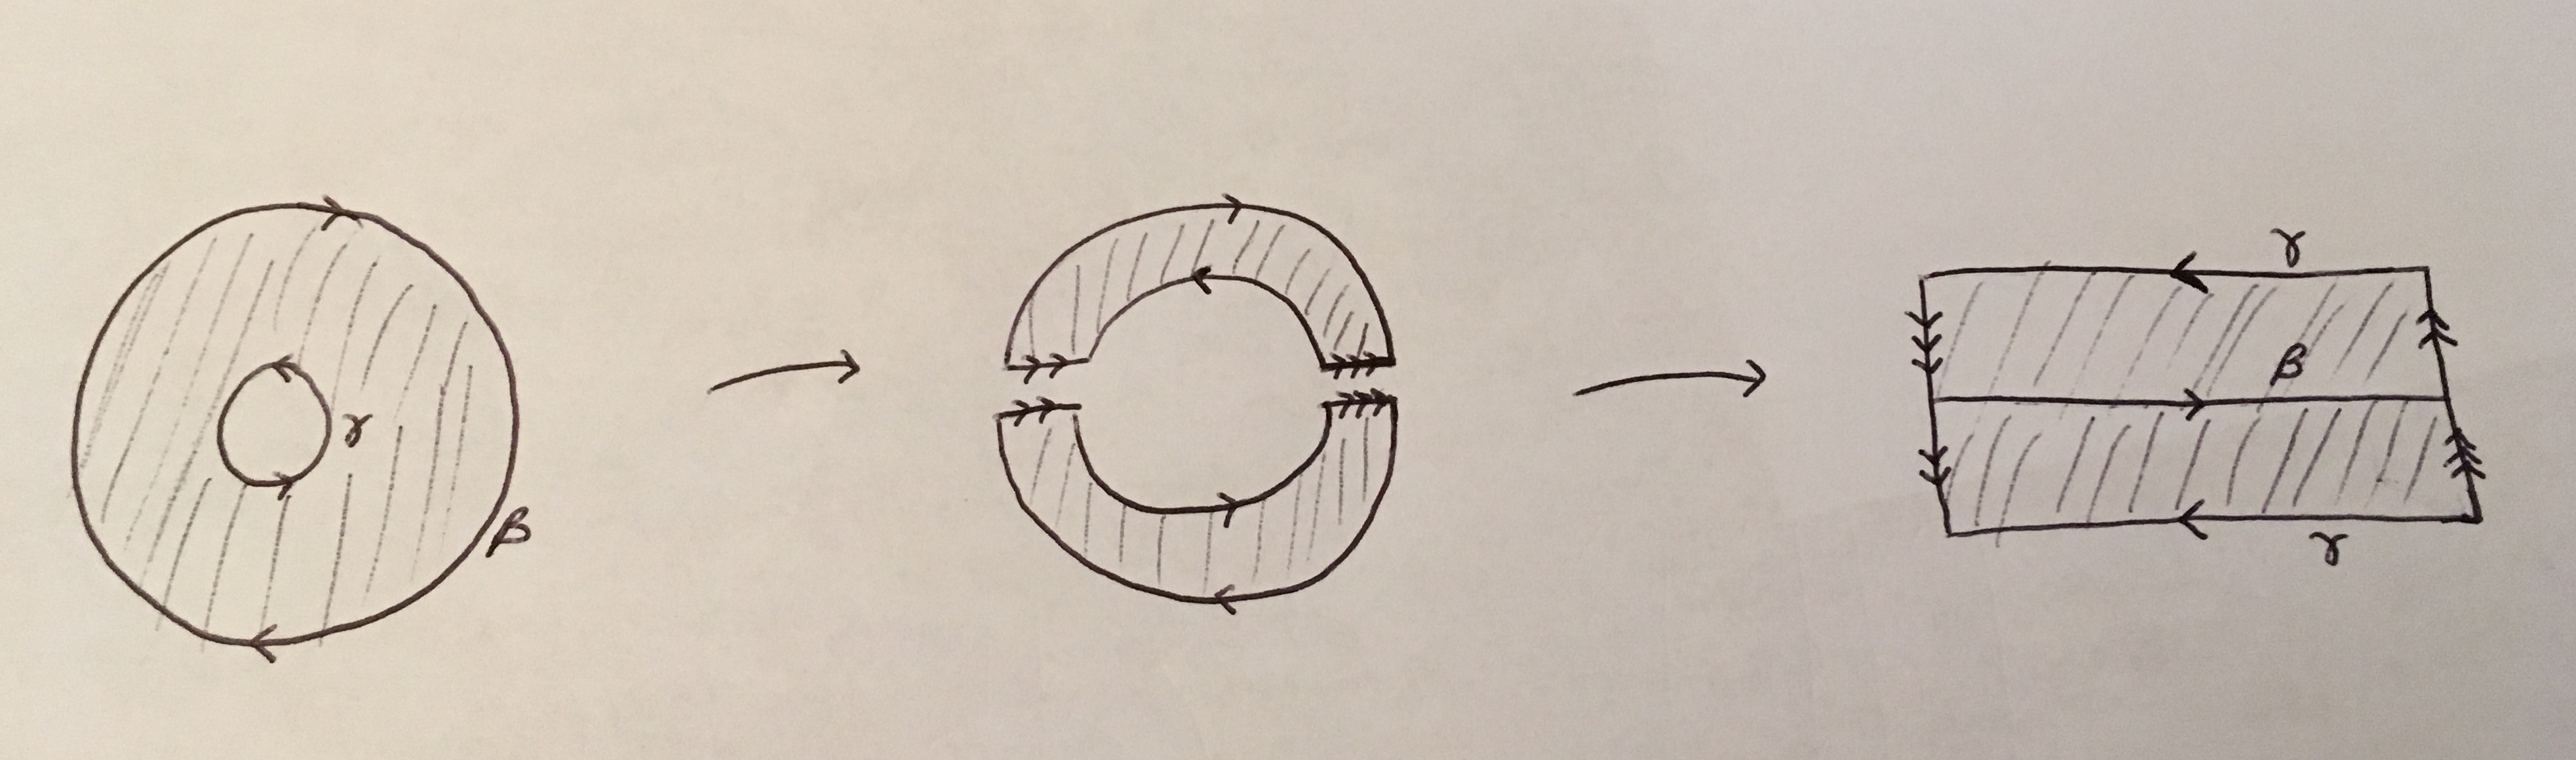
\includegraphics[width=85mm]{RP2.jpg}
\end{figure}
By van Kampen, it follows that $\pi_1(\RP^2) \cong \pi_1(A) \underset{\pi_1(A \cap B)}{\ast} \pi_1(B) \cong \faktor{\langle \beta \rangle}{\langle \beta^2 \rangle} \cong \Z / 2 \Z$.
\end{enumerate}
\end{exmp}

\subsection{Lecture 6}

\begin{definition}
A \textit{knot} is a piecewise smooth embedding of $S^1$ into $\R^3$. Two knots $K_1$ and $K_2$ are \textit{equivalent} if there is some homeomorphism $\varphi : \R^3 \to \R^3$ such that $\varphi(K_1) = K_2$.
\end{definition}

\begin{exmp} $ $
\begin{enumerate}
\item The \textit{unknot} is the standard embedding $S^1 \hookrightarrow \R^3$. 
\item The following space is called the \textit{trefoil knot}.

      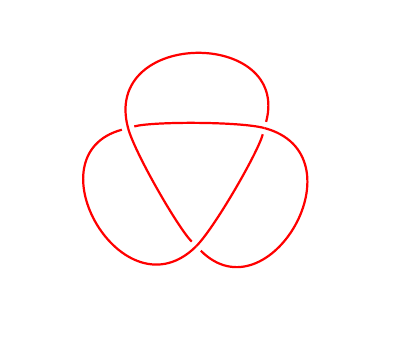
\begin{tikzpicture}
        \foreach \brk in {0,1,2} {
          \begin{scope}[rotate=\brk * 120]
            \node[knot crossing, transform shape,
            inner sep=1.5pt] (k\brk) at (0,-1) {};
          \end{scope}
        }
        \foreach \brk in {0,1,2} {
          \pgfmathparse{int(Mod(\brk - 1,3))}
          \edef\brl{\pgfmathresult}
          \draw[thick,red] (k\brk) .. controls (
          k\brk.4 north west) and (k\brl.4 north east) .. (k\brl.center);
          \draw[thick,red] (k\brk.center) .. controls (k\brk.16 south west) and (k\brl.16 south east) .. (k\brl);
        }
      \end{tikzpicture}
\end{enumerate}
\end{exmp}

\begin{lemma}
The \textit{knot group} $ \pi_1(\R^3 \setminus K)$ is isomorphic to $\pi_1(S^3 \setminus K)$. 
\end{lemma}
\begin{proof}
Recall that $S^3 \cong \R^3 \cup \{\infty\}$. Write $S^3 \setminus K$ as the union of $\R^3 \setminus K$ and the open ball $B\coloneqq  (\R^3 \setminus D) \cup \{\infty\}$ where $D\supset K$ is a sufficiently large disk. Then both $B \cap (\R^3 \setminus K)$ and $B$ are simply connected (the former being homeomorphic to $S^2 \times \R$). By van Kampen, $\pi_1(S^3 \setminus K) \cong \pi_1(\R^3 \setminus K)$. 
\end{proof}

\begin{note}
We have that $S^3 \cong ST_1 \cup_T ST_2$ where $ST_1$ and $ST_2$ denote solid tori with common boundary a torus. Indeed, 
\begin{align*}
 S^3 & = \left\{(z_1, z_2) \in \C^2 \mid \lvert{z_1}\rvert^2 + \lvert{z_2}\rvert^2 =1\right\}
\\  ST_1 &= \left\{(z_1, z_2) \in S^3 \mid \lvert{z_1}\rvert^2 \leq \frac{1}{2}\right\} \cong D^2 \times S^1
\\  ST_1 &= \left\{(z_1, z_2) \in S^3 \mid \lvert{z_2}\rvert^2 \leq \frac{1}{2}\right\} \cong S^1 \times D^2
\\  ST_1 \cap ST_2 &= \left\{(z_1, z_2)\in \C^2 \mid \lvert{z_1}\rvert^2 = \lvert{z_2}\rvert^2 = \frac{1}{2}\right\} \cong S^1\times S^1
.\end{align*}
\end{note}

\bigskip

\begin{definition}
Let $M^n$ be a manifold. A \textit{foliation of $M$} is a collection $\{\L_{\alpha}\}_{\alpha \in A}$ of immersed submanifolds of fixed dimension $l$, called \textit{leaves}, such that $M = \coprod_{\alpha \in A}\L_{\alpha}$ and for each $p\in M$, there is some smooth chart $(U, \varphi)$ around $p$ with $\varphi(\L_{\alpha} \cap U) \subset \R^l$ for each $\alpha$.
\end{definition}

\begin{exmp} $ $
\begin{enumerate}
\item The collection of circles $\left\{ \{q\} \times S^1\right\}_{q\in S^1}$ forms a foliation of the torus. 
\item For each $\theta \in \R$, define the curve in the torus $\gamma_{\theta}(t) = \left(e^{it}, e^{i(\alpha t + \theta)}\right)$. Then the collection of curves $\{\im{\gamma_{\theta}}\}_{\theta \in \R}$ forms another foliation of the torus. If $\theta \in \Q$, then each curve is an embedded circle. Otherwise, it is dense in the torus. 
\end{enumerate}
\end{exmp}

\begin{theorem}
The torus is the only surface that admits a foliation. 
\end{theorem}

Nevertheless, the so-called Reeb torus demonstrates that there are foliations on $S^3$. 

\medskip

Now if $M = \coprod_{\alpha} \L_{\alpha}$, then $\L \coloneqq  \bigcup_{x\in M} T_x \L_{\alpha_x}$ (where $x\in L_{\alpha_x}$) is a subbundle of $TM$ such that $X, Y \in C^{\infty}(M, \L) \implies [X, Y] \in \L$. The Frobenius theorem is precisely the converse of this. 


\bigskip

Let us return now to our discussion of knot theory.

\begin{note}[Wirtinger presentation] 
Draw our knot $K$ as follows. Take a finitely many arcs $\alpha_1, \ldots, \alpha_n$ such that each $\alpha_i$ is connected to $\alpha_{i+1} \mod n$. Orient the knot so that the arcs are labeled in the direction of the orientation. Draw a short arrow $x_i$ passing under each $\alpha_i$ from right to left. The $x_i$ represent loops starting at a base point going under the arc from its base to head and back to base. At each crossing, we get a relation among the $x_i$ as follows.
\begin{figure}[H]
\centering
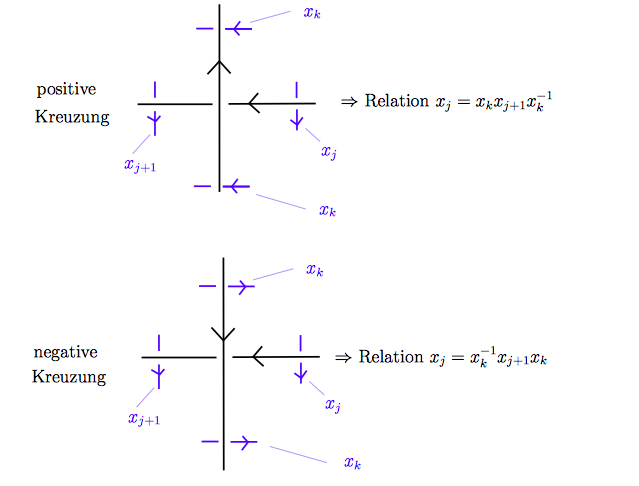
\includegraphics[width=68mm]{Wirtinger_presentation.png}
\end{figure}
For each $i$, let $r_i$ denote the relation $x_kx_i = x_{i+1}x_k$.
\end{note}

\begin{prop}
$\pi_1(S^3 \setminus \text{unknot})\cong \Z$.
\end{prop}

\begin{theorem}
$\pi_1(\R^3 \setminus K, \ast) \cong \langle x_1, \ldots, x_n \mid r_1, \ldots, r_n \rangle$.
\end{theorem}
\begin{proof}
We may embed each arc $\alpha_i$ in the plane $z=0$ except for a small vertical segment at each end of the arc, which will lie instead in the plane $z={-1}$. 
\[
\begin{tikzpicture}
  \draw (0,1) node (nodeA) [below]  {} -- (4,1) node (nodeB) [above] {} node [midway, above, sloped] (EdgeAB) {$\alpha_i$} -- (4,0) node [below] (nodeC) {} node [midway, above, sloped] (EdgeBC) {} -- (6,0) node [above] (nodeD) {} node [midway, below, sloped] (EdgeCD) {$\beta_i$} -- (6,1) node (nodeE) [below]  {} -- (10,1) node (nodeF) [below]  {} node [midway, above, sloped] (EdgeEF) {$\alpha_{i+1}$} 
(4,-2) node (nodeG) [below]  {} --  (6,3) node (nodeH) [below]  {};
\end{tikzpicture}
\]
Let $A = \{z\geq 1 \}\setminus K$. 
The lower boundary of $A$ is  the union of the $n$ line segments with each $\beta_i$ removed. For each $i=1\leq i \leq n$, let $B_i$ equal the union of a solid rectangular box whose top lies on $z={-1}$ surrounding but excluding $\beta_i$ and an arc connection $\beta_i$ to $\ast$. Make the $B_i$ disjoint. Let $C$ equal the closure of everything below the $B_i$. 
Then  we can write $$\R^3 \setminus K = A \cup B_1 \cup \cdots \cup B_n \cup C.$$ We see that $\pi_1(A, \ast) \cong \mathbb{F}_n$, $\pi_1(B_1) =0$, and $C$ is contractible. Now, $A \cap B_1$ equals a rectangle minus $\beta_1$ together with an arc connecting $\beta_1$ to $\ast$. Thus, $A \cap B_1 \simeq S^1$. Write $\pi_1(A \cap B_1) = \langle \gamma_1 \rangle \cong \Z$. But \hl{$i_{AB_1}(\gamma) = x_1x_k^{-1}x_2^{-1}x_k$.} By van Kampen, we get $\pi_1(A \cup B_1) \cong \faktor{\mathbb{F}_n}{(r_1)}$. By induction, it follows that $$\pi_1(A \cup B_1 \cup \cdots \cup  B_n) \cong \mathbb{F}_n/(r_1, \ldots, r_n).$$ Finally, since $C$ is contractible, we get $\pi_1(A \cup B_1 \cup \cdots \cup  B_n \cup C) \cong \pi_1(A \cup B_1 \cup \cdots \cup  B_n).$
\end{proof}

\subsection{Lecture 7}

\begin{remark} If $G = \langle g_1, \ldots, g_n \mid w_1, \ldots, w_m \rangle$, then $G \cong \faktor{\F(g_1, \ldots, g_n)}{N}$ where $N$ denotes the normal subgroup generated by $w_1, \ldots, w_m$ and each $w_i$ is a word in $g_1, \ldots, g_n$. 
Now, let $G_1 = \langle g_1, \ldots, g_n \mid w_1, \ldots, w_m \rangle$ and $G_2 = \langle h_1, \ldots, h_k \mid u_1, \ldots, u_l \rangle$
It is known that the following two problems are undecidable.
\begin{enumerate}[label=(\alph*)]
\item{(isomorphism problem)} Is $G_1 \cong G_2$?
\item {(word problem)} Given a word $w$ over $\left\{g_1, \ldots, g_n\right\}$, is $w=e$? 
\end{enumerate}
\end{remark}

\bigskip

\begin{exmp}
Let $S_g$ denote the (closed) orientable surface of genus $g$. Note that $S_g \cong S_{g-1} \# T$. We can draw $S_g$ as an oriented  $4g$-gon with pairs of sides identified as follows.

\[
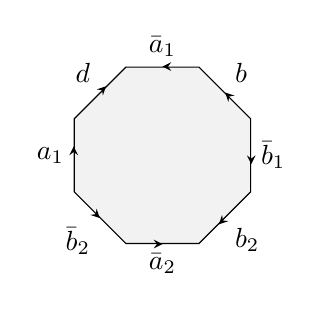
\begin{tikzpicture}


\node[fill=gray!10] (pol) [
  draw,
  minimum size=0.2\textwidth,
  regular polygon, regular polygon sides=8,
  ]{};
\foreach \x/\y/\i in {1/2/1} %\alpha's
  \path[auto=right, ->-]
    (pol.corner \x)--(pol.corner \y)
      node[midway]{$\bar{a}_1$};
\foreach \x/\y/\i in {3/4/1} %inverse \alpha's
   \path[auto=right, -<-]
     (pol.corner \x)--(pol.corner \y)
     node[midway]{$a_1$};
\foreach \x/\y/\i in {2/3/1} %\beta's
  \path[auto=right, -<-]
    (pol.corner \x)--(pol.corner \y)
      node[midway]{$d$};
\foreach \x/\y/\i in {4/5/1} %inverse \beta's
   \path[auto=right, ->-]
     (pol.corner \x)--(pol.corner \y)
     node[midway]{$\bar{b}_2$};
      \foreach \x/\y/\i in {5/6/1} %inverse \beta's
   \path[auto=right, ->-]
     (pol.corner \x)--(pol.corner \y)
     node[midway]{$\bar{a}_2$};
      \foreach \x/\y/\i in {6/7/1} %inverse \beta's
   \path[auto=right, -<-]
     (pol.corner \x)--(pol.corner \y)
     node[midway]{$b_2$};
      \foreach \x/\y/\i in {7/8/1} %inverse \beta's
   \path[auto=right, -<-]
     (pol.corner \x)--(pol.corner \y)
     node[midway]{$\bar{b}_1$};
 \foreach \x/\y/\i in {8/1/1} %inverse \beta's
   \path[auto=right, ->-]
     (pol.corner \x)--(pol.corner \y)
     node[midway]{$b$};

 
\end{tikzpicture}
\]

For example, $a_1 \sim \bar{a}_1$. 
Then we can decompose $S_g$ into a small disk $A$ around the origin and an annulus-like space $B$ so that $A \cap B$ is a smaller annulus bounded above by the boundary of $A$ and below by the inner boundary of $B$. Then $\pi_1(A \cap B) \cong \langle \gamma \rangle$ where $\lvert{\gamma}\rvert =\infty$. Further, $\pi_1(A) = 0$, and $$\pi_1(B) \cong \underset{\{1,2, \ldots, 2g\}}{\ast} \Z$$ since $B$ deformation retracts onto a bouquet of $2g$ circles. Observe that $i_{BA}(\gamma) = \prod_{i=1}^{g}[a_i, b_i]$, which implies that $$ \pi_1(S_g) \cong \big \langle a_1, \ldots, a_g, b_1, \ldots, b_g \mid    \prod_{i=1}^{g}[a_i, b_i] =1 \big  \rangle .$$
\end{exmp}

\smallskip

\begin{note}
The comb space is path connected but not locally path connected. 
\end{note}

\smallskip

\begin{lemma}
If $p: \left(Y, y_0\right) \to \left(X, x_0\right)$ is a covering projection, then there is an isomorphism of sets $$p^{-1}(x_0) \overset{\cong}{\longrightarrow} \faktor{\pi_1\left(X, x_0\right)}{p_{\ast}\pi_1\left(Y, y_0\right)}.   $$
\end{lemma}
\begin{proof}
Let $\gamma$ be a loop in $\left(X, x_0\right)$. Lift it to $\tilde{\gamma}$ such that $\tilde{\gamma}(0) = y_0$. Set $\alpha(\gamma) = \tilde{\gamma}(1) \in p^{-1}(x_0)$. The map $\alpha : \faktor{\pi_1\left(X, x_0\right)}{p_{\ast}\pi_1\left(Y, y_0\right)} \to p^{-1}(x_0)$ is well-defined since $\widetilde{h \ast \gamma} = \tilde{h} \ast \tilde{\gamma}$ when $[h] \in p_{\ast}\pi_1\left(Y, y_0\right)$. It is surjective because $Y$ is path connected. If $\alpha(\gamma_1) = \alpha(\gamma_2)$, then $\tilde{\gamma}_1\ast \tilde{\gamma}_2^{-1}= \widetilde{\gamma_1 \ast \gamma_2^{-1}}$ is a loop in $\left(Y, y_0\right)$, so that $\gamma_1 \ast \gamma_2^{-1}  \in p_{\ast}\pi_1\left(Y, y_0\right)$. This shows that $\alpha$ is injective as well.
\end{proof}

\begin{lemma}[Lifting criterion]\label{LC}
Let $p: \left(Y, y_0\right) \to \left(X, x_0\right)$ be a covering projection and $f: (Z, z_0) \to \left(X, x_0\right)$ a map with $Z$ path connected and locally path connected.  Then there exists some map $\tilde{f}$ fitting into a commutative diagram \[
\begin{tikzcd}
 & Y \arrow[d, "p"] \\
Z \arrow[r, "f"'] \arrow[ru, "\tilde{f}", dashed] & X
\end{tikzcd}
\] if and only if  $f_{\ast}\pi_1(Z, z_0) \subset p_{\ast} \pi_1\left(Y, y_0\right) \subset \pi_1\left(X, x_0\right)$. 
\end{lemma}
\begin{proof} $ $

\smallskip

($\Longrightarrow$) Simply notice that $f_{\ast} = \left(p\tilde{f}\right)_{\ast}= p_{\ast}\tilde{f}_{\ast}$.

\medskip

 
($\Longleftarrow$) Let $z\in Z$. Find some path $\gamma : z_0 \leadsto z$.  Then $f \gamma$ is a path in $X$ starting at $x_0$. There exists a unique lift $\widetilde{f \gamma}$ starting at $y_0$. Set $\tilde{f}(z) = \widetilde{f \gamma}(1)$. We must check that $\tilde{f}$ is well-defined. Let $\gamma' : z_0 \leadsto z$. Then $h_0\coloneqq (f \gamma ')\ast (f\gamma)^{-1}$ is a loop at $x_0$. Note that $[h_0] \in f_{\ast}\pi_1(Z, z_0) \subset p_{\ast} \pi_1\left(Y, y_0\right)$. Hence there is some homotopy $H: h_0 \simeq_p p \circ \tilde{h}_1$ for some loop $\tilde{h}_1$ at $y_0$. Apply \cref{HLP} to get a homotopy $\widetilde{H} : \tilde{h}_0 \simeq_p \tilde{h}_1$, so that $\tilde{h}_0$ is a loop. By uniqueness of lifts, $\tilde{h}_0 =\widetilde{f \gamma '}\ast \widetilde{f\gamma}^{-1}$, which implies that $\widetilde{f \gamma '}(1) = \widetilde{f\gamma}(1-0) = \widetilde{f\gamma}(1)$, as required.

\medskip

 It remains to verify that $\tilde{f}$ is continuous. Find some path $\lambda : z_0 \leadsto z$. We know that there is some neighborhood $U \ni f(z)$ that is is evenly covered by $p$. Let $\widetilde{U}$ denote the sheet containing $\tilde{f}(z)$ and find some homeomorphism $p : \widetilde{U} \to U $. Find some path connected neighborhood $V\ni z$ such that $f(Z) \subset U$. Let $z' \in V$. Find some path $\eta : z \leadsto z'$. Then the path $(f \lambda )\ast (f \eta)$ lifts to $\left(\widetilde{f \lambda}\right) \ast \left(\widetilde{f \eta}\right)$ where $\widetilde{f\eta} = p^{-1}f\eta$. As $z'$ was arbitrary in $V$, this implies that $\tilde{f}\restriction_V =p^{-1}f\restriction_V$, which is continuous. Hence $\tilde{f}$ is continuous as well. 
\end{proof}

\begin{prop}[Unique lifting property]\label{ULP}
Let $p: Y \to X$ be a covering projection and $f: Z \to X$ a map with $\tilde{f}_1, \tilde{f}_2 : Z \to Y$ lifts of $f$. Let $Z$ be connected. If there is some $z_0 \in Z$ such that $\tilde{f}_1(z_0) = \tilde{f}_2(z_0)$, then $\tilde{f}_1 =  \tilde{f}_2$.
\end{prop}

\begin{question}
Let $X$ be a space with  $\pi_0(X) =0$. When is there a locally path connected covering space $p: \widetilde{X} \to X$ such that $\pi_1\left(\widetilde{X}\right) =0$? 
\end{question}

Suppose that such a space exists. Let $x \in X$. Suppose that the open set $U \subset X$ with $x\in U$ is evenly covered. Ley $\widetilde{U} \subset \widetilde{X}$ be one sheet.  If $\gamma$ is a loop in $U$, then it lifts to a loop $\tilde{\gamma}$ at, say, $y \in \widetilde{U}$, which must be nullhomotopic. Find some homotopy $H: \tilde{\gamma} \simeq_p c_y$. Then $pH : \gamma \simeq_p c_x$. Therefore, for any $x\in X$, there is some neighborhood $U\ni x$ such that $\pi_1(U) =0$.
Such a property of $X$ is called being \textit{semilocally simply connected}. 


\begin{theorem}
Suppose that $X$ is path connected, locally path connected, and semilocally simply connected (hereafter ``swell"). Then there is some covering projection $p: \widetilde{X} \to X$ such that $\widetilde{X}$ is simply connected. 
\end{theorem}
\begin{proof}
Pick $x_0 \in X$. Let $P_{x_0} \coloneqq  \{\gamma : I \to X \mid \gamma(0) = x_0\}$. Set $\widetilde{X} = \faktor{P_{x_0}}{\simeq_p}$, endowed with the compact-open topology. 
\end{proof}

\begin{lemma}
Let $X$ be a swell space.  If $Y_1, Y_2 \overset{p_1, p_2}{\longrightarrow} X$ are two simply connected covering spaces, then they are \textit{isomorphic} in the following sense. There is some homeomorphism $\psi : Y_2 \to Y_1$ such that 
\[
\begin{tikzcd}
Y_1 \arrow[d, "p_1"'] & Y_2 \arrow[ld, "p_2"] \arrow[l, "\psi"'] \\
X & 
\end{tikzcd}
\] commutes (i.e., $\psi$ is a bundle isomorphism).
\end{lemma}
\begin{proof}
By \cref{LC}, we can obtain lifts
\[
\begin{tikzcd}
 & Y_2 \arrow[d, "p_2"] \\
Y_1 \arrow[r, "p_1"'] \arrow[ru, "\tilde{p}_1", dashed] & X \\
 & Y_1 \arrow[d, "p_1"] \\
Y_2 \arrow[r, "p_2"'] \arrow[ru, "\tilde{p}_2", dashed] & X
\end{tikzcd}.
\] Then $\tilde{p}_2\tilde{p}_1 = \1_{Y_1}$ since $p_1$ has a unique lift. Similarly, $\tilde{p}_1\tilde{p}_2 = \1_{Y_2}$. Hence $\tilde{p}_2 : Y_2 \overset{\cong}{\longrightarrow} Y_1.$ 
\end{proof}

\subsection{Lecture 8}


If $X$ is a swell space, then we call such a cover $p: \left(\widetilde{X}, \tilde{x}_0\right) \to \left(X, x_0\right)$ the \textit{universal cover of $X$}. It is universal in that for any path connected covering space $p': \left(Y, y_0\right) \to \left(X, x_0\right)$, there exists a unique covering projection $p'': \left(\widetilde{X}, \tilde{x}_0\right) \to \left(Y, y_0\right)$ such that $p'' p' = p$. 


\begin{lemma}
Let $X$ be swell. For any subgroup $H \leq \pi_1\left(X, x_0\right)$, there exists a path connected covering space $p_H : X_H \to X$ such that $p_H (\pi_1(X_H, h_H)) = H$.
\end{lemma}
\begin{proof}
Define an equivalence relation $\sim$ on the universal cover $p: \widetilde{X} \to X$ as follows. Let $y_1 \sim y_2$ if $p(y_1) = p(y_2)$ and for any two paths $\gamma_1$ and $\gamma_2$ from $x_0$ to $y_1$ and $y_2$, respectively, $(p\gamma_1)\ast (p\gamma_2)^{-1}\in H$. Set $X_H = \faktor{\widetilde{X}}{\sim}$ and note that the map $p_H : X_H \to X$ given by $[y] \mapsto p(y)$ is a covering space. Set $x_H= q(\tilde{x}_0)$ where $q: \widetilde{X} \to X_H$ denotes the natural projection. We know that $p_H \pi_1(X_H, x_H)$ consists of loops $\gamma$ in $\left(X, x_0\right)$ whose lifts to $X_H$ are also loops.  If $\tilde{\gamma}$ denotes the lift of $\gamma$ to $\widetilde{X}$, then we see that $$\tilde{\gamma}(1) \sim \tilde{x}_0 \iff p_H(\tilde{\gamma}^{-1} c_{\tilde{x} _0}) \in H,$$ meaning that  $p_H \circ \tilde{\gamma}$ is a loop at $x_0$ if and only if $\gamma$ belongs to $H$.
\end{proof}

\begin{lemma}
Let $X$ be path connected and locally path connected. Suppose that $p_1:(Y_1, y_1) \to \left(X, x_0\right)$ and $p_2 : (Y_2, y_2) \to \left(X, x_0\right)$ are two (path connected) covering projections. Then there exists an isomorphism $\varphi : (Y_1, y_1) \to (Y_2, y_2)$ if and only if  $$p_{1\ast} \pi_1(Y_1, y_1) = p_{2 \ast} \pi_1(Y_2, y_2).$$
\end{lemma}
\begin{proof} $ $
\smallskip

 ($\Longrightarrow$)

This follows from the fact that $p_1 = p_2f$ and $p_2 = p_1f^{-1}$. 

\medskip

 ($\Longleftarrow$) 
 
 Apply \cref{LC} twice to lifts $\tilde{p}_1$ and $\tilde{p}_2$ such that $p_2\tilde{p_1} = p_1$ and $p_1\tilde{p_2}=p_2$. By \cref{ULP}, $\tilde{p}_1\tilde{p}_2=\1$ and $\tilde{p}_2\tilde{p}_1 = \1$. Hence $\tilde{p}_1$ and $\tilde{p}_2$ are inverse isomorphisms. 
\end{proof}

\begin{corollary}
Let $X$ be swell. There is a bijection between the set of isomorphism classes of path connected covering spaces $p: (Y, y) \to \left(X, x_0\right)$ of $X$ and the set of subgroups of $\pi_1\left(X, x_0\right)$ given by $$(Y, y) \longleftrightarrow p_{\ast}\pi_1(Y, y)    .$$
\end{corollary}

\smallskip

Let $p: \widetilde{X} \to X$ be a covering space. The set of isomorphisms $\widetilde{X}  \to \widetilde{X} $, called \textit{deck transformations}, forms a group $G(\widetilde{X})$ under composition. This corresponds to the Galois group in algebra.

By \cref{ULP}, if $\widetilde{X}$ is path connected, then any $f\in G(\widetilde{X})$ is entirely determined by its value at a single point.

\begin{definition}
A covering space $p:Y \to X$ is \textit{normal} if $G(Y)$ acts transitively on the set $p^{-1}(x)$ for each $x\in X$.
\end{definition}

\begin{lemma}
Let $p: \left(Y, y_0\right) \to \left(X, x_0\right)$ be a path connected covering space with $X$ swell. Let $H\coloneqq  p_{\ast}\pi_1\left(Y, y_0\right)$. Then 
\begin{enumerate}
\item $p$ is normal if and only if $H \unlhd \pi_1\left(X, x_0\right)$.
\item $G(Y) \cong \faktor{N(H)}{H}$. 
\end{enumerate}
\end{lemma}
\begin{proof} $ $
\begin{enumerate}
\item For any $y_1 \in p^{-1}(x_0)$, there is some path $\eta : y_0 \leadsto y_1$. Then $\pi_1\left(Y, y_0\right) \cong \pi_1(Y, y_1)$ via the map $[\gamma] \mapsto \eta^{-1} \gamma \eta$. Note that $p \eta \in \pi_1\left(X, x_0\right)$ and that $p_{\ast} \pi_1\left(Y, y_0\right) = [p \eta]p_{\ast} \pi_1(Y, y_1) [p\eta]^{-1}$. Hence $[\gamma] \in N(H) \iff  p_{\ast} \pi_1\left(Y, y_0\right) = p_{\ast} \pi_1(Y, y_1)$ where $\gamma$ lifts to a path $y_0 \leadsto y_1$. By \cref{LC} together with \cref{ULP}, it follows that $[\gamma] \in N(H)$ if and only if there is some deck transformation $Y \to Y$ mapping $y_0$ to $y_1$. Hence $N(H) = \pi_1\left(X, x_0\right)$ if and only if $p$ is normal. 
\item Define $\varphi : N(H) \to G(Y)$ by mapping $[\gamma]$ to the deck transformation sending $y_0$ to $y_1$. The preceding argument shows that $\varphi$ is surjective. Further, $\ker{\varphi}$ consists of loop at $x_0$ whose lifts are loops in $Y$. Thus, $\ker{\varphi} = H$. 
\end{enumerate}
\end{proof}

Therefore, $G(Y) \cong \faktor{\pi_1\left(X, x_0\right)}{H}$ when $p$ is normal.

\begin{exmp}
If $\Gamma$ acts freely and properly discontinuously on the space $Y$, then the quotient map $Y \to \faktor{Y}{\Gamma}$ is a normal covering space such that $\Gamma \cong G(Y)$. Hence $\Gamma \cong \faktor{\pi_1\left(X, x_0\right)}{p_{\ast}\pi_1\left(Y, y_0\right)}$ where $X\coloneqq  \faktor{Y}{\Gamma}$.
\end{exmp}

\begin{definition}
A \textit{graph} is a $1$-dimensional CW-complex. 
\end{definition}

\begin{lemma}
Let $G$ be a graph.  Then $\pi_1(G)$ is a free group.
\end{lemma}
\begin{proof}
Since every tree is contractible, we see that $G$ is homotopy equivalent to a wedge sum of circles by noting that $\bigvee_{\alpha} S_{\alpha}^1 \simeq \faktor{G}{T}\simeq G$ where $T$ is a maximal tree contained in $G$. 
\end{proof}

\begin{note}
If $X$ is a graph and $p: Y \to X$ is a covering space, then $Y$ is also a graph. 
\end{note}

\begin{theorem}[Nielsen-Schreier]
Let $\Gamma$ be a free group and $H\leq \Gamma$. Then $H$ is free. 
\end{theorem}
\begin{proof}
We have that $\Gamma \cong \pi_1(X)$ where $X\coloneqq  \bigvee_{\alpha} S_{\alpha}^1$. Also, $H$ corresponds to some covering space $p: Y \to X$. Therefore, $Y$ is a graph, and $\pi_1(Y)$ is free. This implies that $H= p_{\ast}\pi_1(Y)$ is free since $p_{\ast}$ is injective. 
\end{proof}

\section{Homology} 

The \textit{standard $k$-simplex} is the set $$  \Delta^k \equiv \left\{(t_0, \ldots, t_k) \mid \sum t_i = 1, \ t_i \geq 0 \right\} = \left\{(x_1, \ldots, x_n) \mid 0\leq x_1 \leq x_2 \leq \cdots \leq x_k \leq 1 \right\} .$$
For each $i=0, \ldots, k+1$, define the \textit{face map} $\partial^i : \Delta^k \to \Delta^{k+1}$ by $(t_0, \ldots, t_k) \mapsto (t_0, \ldots, t_{i-1}, 0, t_i, \ldots, t_k)$.

\begin{definition} 
 An \textit{(abstract) simplicial complex} is a set $K$ together with a collection of finite subsets $\Sigma \subset P(K)$ such that if $\sigma \in \Sigma$ and $\tau \subset \sigma$, then $\tau \in \Sigma$. 
 
 If $\sigma \in \Sigma$ and $\lvert{\sigma}\rvert= k$, then $\sigma$ is called a \textit{$(k-1)$-simplex}.  An \textit{ordered simplex} is a simplex equipped with an ordering of its vertices.  Any subset of a simplex is called a \textit{face}.
\end{definition}


Let $(K, \Sigma)$ be a simplicial complex. Let $S$ denote the set of ordered $k$-simplices in $K$. Let $$C_k(K, \Sigma) \coloneqq \faktor{\bigoplus_{s\in S} \Z}{\sim}$$ where  $v_0\cdots v_k \sim ({-1})^{\tau} v_{\tau(0)}\cdots v_{\tau(k)}$ for any $\tau \in S_{k+1}$.


\begin{note}
$C_k(K, \Sigma)$ is a free abelian group.
\end{note}

\begin{definition}
Define the \textit{differential} $\partial_{k} : C_k(K, \Sigma) \to C_{k-1}(K, \Sigma)$ by  $$\partial_{k}(v_0\cdots v_k) = \sum_{i=0}^k ({-1})^i v_0 \cdots \widehat{v_i} \cdots v_k, $$ which we extend by linearity.  
\end{definition}

\begin{exercise}
Show that $\partial^2 =0$.
\end{exercise}

\begin{exmp}
$v_0v_1v_2 \overset{\partial_2}{\longmapsto}  v_1 v_2 - v_0v_2 + v_0v_1  \overset{\partial_1}{\longmapsto} v_2 - v_1 -(v_2 - v_0) + v_1 - v_0 =0 .$
\end{exmp}

\begin{definition}
Define the \textit{$k$-th homology group of $(K , \Sigma)$} as $$H_k(K, \Sigma) = \faktor{\ker{\partial_k}}{\im{\partial_{k+1}}}.$$ We call $Z_k(K, \Sigma)\coloneqq  \ker{\partial_k}$ \textit{cycles} and $B_k(K, \Sigma)\coloneqq  \im{\partial_{k+1}}$ \textit{boundaries}.
\end{definition}

\subsection{Lecture 9}


The category of simplicial complexes $\Delta$ has as morphisms functions $f: \left(K, \Sigma_K\right) \to \left(L, \Sigma_L\right)$ such that $\sigma \in \Sigma_K \implies f(\sigma) \in \Sigma_L$. We call these \textit{simplicial maps}.


\begin{definition}
A \textit{subcomplex of $K$} is a subset $L \subset K$ such that inclusion is a simplicial map.
\end{definition}

\begin{exmp}
If $\left(K, \Sigma_K\right)$ is a simplicial complex, then $K$ together with $K^p \coloneqq   \left\{\sigma \in \Sigma_K : \lvert{\sigma}\rvert \leq p+1\right\}$ is a subcomplex.
\end{exmp}

\smallskip

If $K$ is a simplicial complex, then define $\lvert{K}\rvert$ as the set $$\left\{\alpha : K \to I \mid \sum_{v\in K} \alpha(v)=1 \land \{v \mid \alpha(v) \ne 0\} \in \Sigma_K\right\}.$$ Let $\lvert{K}\rvert_d$ denote this set endowed with the topology induced by the metric given by $$d(\alpha, \beta) = \sqrt{\sum_{v\in K} \lvert{\alpha(v) -\beta(v)}\rvert^2} .$$


\begin{exmp}
Let  $K= \{0, 1, \ldots, n\}$ and let $\Sigma$ consist of all finite subsets of $K$. Then $$\lvert{K}\rvert_d = \left\{ (\alpha(0), \ldots, \alpha(n)) \mid \alpha(0) + \cdots + \alpha(n) = 1\right\} \cong_{\mathbf{Set}} \Delta^n,$$ which recovers the Euclidean metric. 
\end{exmp}

\begin{note} $ $
\begin{enumerate}
\item When $\sigma \in \Sigma_K$ is a $q$-simplex, there exists a natural map $\lvert{\sigma^q}\rvert_d : \Delta^q \to \lvert{K}\rvert_d$  given by mapping $x$ to the function $\alpha$ where $\alpha(\sigma) =x$ and $\alpha(v) = 0$ for any $v\notin \sigma$.  
\item Define a new topology on $\lvert{K}\rvert$ where $A\subset \lvert{K}\rvert$ is closed (resp. open) if $(\lvert{\sigma}\rvert_d)^{-1}(A)$ is closed (resp. open) in $\Delta^{\lvert{\sigma}\rvert -1}$ for each $\sigma \in \Sigma_K$. From now on, $\lvert{K}\rvert$ is assumed to have this topology. 
\item Given a simplicial map $f: K \to L$, define the map $\lvert{f}\rvert : \lvert{K}\rvert \to \lvert{L}\rvert$ by $\alpha \mapsto \left(w \mapsto \sum_{v\in f^{-1}(w)} \alpha(v)\right)$. Thus, we get a functor $\lvert{\cdot}\rvert : \Delta \to \mathbf{Top}$.
\end{enumerate}
\end{note}

\begin{definition}
A \textit{triangulation of a space $X$} is a pair $((K, \Sigma), \varphi)$ such that $\varphi : \lvert{K}\rvert \to X$ is a homeomorphism. 
\end{definition}

\begin{remark}
The Cantor set has no triangulation. 
\end{remark}

\begin{definition}
The category of \textit{chain complexes $\ch$} has as objects sequences of abelian groups of the form 
\[
\begin{tikzcd}
A_0 & A_1 \arrow[l, "\partial_1"'] & A_2 \arrow[l, "\partial_2"'] & A_3 \arrow[l, "\partial_3"'] & \cdots \arrow[l, "\partial_3"']
\end{tikzcd}
\] such that $\partial_i\partial_{i+1} =0$ for each $i\in \N$. Its morphisms are commutative diagrams of the form
\[
\begin{tikzcd}
A_0 \arrow[d, "f_0"] & A_1 \arrow[l, "\partial_1"'] \arrow[d, "f_1"] & A_2 \arrow[l, "\partial_2"'] \arrow[d, "f_2"] & A_3 \arrow[l, "\partial_3"'] \arrow[d, "f_3"] & \cdots \arrow[l, "\partial_4"'] \\
B_0 & B_1 \arrow[l, "\partial'_1"] & B_2 \arrow[l, "\partial'_2"] & B_3 \arrow[l, "\partial'_3"] & \cdots \arrow[l, "\partial'_4"]
\end{tikzcd}
,\] so that  $\partial_{i-1}f_i = f_{i-1}\partial_{i-1}$ for each $i$. In this case, we call $f\coloneqq  \left(f_i\right)_{i\in \Z}$ a \textit{chain map}.
\end{definition}

\begin{definition} $ $
\begin{enumerate}
\item Given a chain complex $\left(A, \partial\right)$, define its \textit{$i$-th homology group} as $$ H_i(A, \partial) \equiv \faktor{Z(A_i)}{B(A_i)} $$ where $\underbrace{Z_i \coloneqq  \ker{\partial_{i}}}_{\textit{cycles}}$ and $\underbrace{B_i \coloneqq  \im{\partial_{i+1}}}_{\textit{boundaries}}$. 
\item Any morphism $f: (A, \partial) \to (B, \partial ')$ induces a map $H_q(f) : H_q(A) \to H_q(B)$. We say that $f$ is a \textit{quasi-isomorphism} if $H_q(f)$ is an isomorphism for each $q$. 
\end{enumerate}
\end{definition}

\begin{note} $ $
\begin{enumerate}
\item Any chain map preserves both cycles and boundaries.
\item We have a functor $C_{\bullet}: \Delta \to \ch$ given by $\left(K, \Sigma\right) \mapsto \left(C_q(K, \Sigma), \partial_{q}\right)_{q\geq 0}$. As a result, we find ourselves with the following diagram of functors.
\[
\begin{tikzcd}
\Delta \arrow[d, "C_{\bullet}"'] \arrow[r, "\lvert{\cdot}\rvert"] & \mathbf{Top} \\
\ch \arrow[r, "H_{\bullet}"] & \mathbf{Ab}
\end{tikzcd}
\]
\end{enumerate}
\end{note}

\smallskip

The $\textit{Hauptvermutung}$ is the conjecture that if $X$ is a nice topological space such as a manifold, then for any two triangulations of $X$, you  can get from one to the other in a combinatorial way. It turns out that this is false. Hence we cannot fill our above diagram with a functor $\mathbf{Top} \to \Delta$.

Eilenberg and Steenrod, however, created the following approach to obtain certain reverse arrows in our diagram. Let $X$ be a space. A \textit{singular $q$-simplex on $X$}  is a continuous map $\Delta^q \to X$. Let $\text{Sing}_q(X)$ denote the set of all singular $q$-simplices on $X$. Let $C_q(X)$ be the free abelian group on $\text{Sing}_q(X)$. Define $\partial_{q} : C_q(X) \to C_{q-1}(X)$ by 
$$\sigma \mapsto \sum_{i=0}^q({-1})^i \sigma \restriction_{\left[v_0, \ldots, \widehat{v_i}, \ldots, v_q\right]}$$ 
where $\Delta^q \cong \left[v_0, \ldots, v_q\right]$. Then $\partial_{q-1}\partial_q =0$. We now have a functor $\mathbf{Top} \to \ch$ that maps each map $f: X \to Y$ of spaces to the chain map $(f_n)$ where $f_n(g: \Delta^n \to X) = f \circ g_n$. Note that the induced homology functor $\mathbf{Top} \to \mathbf{Ab}$ is a topological invariant. 

\smallskip




\begin{definition}
Let $(A, \partial)$ and $(B, \partial)$ be two chain complexes and $f,g : (A, \partial_A) \to (B, \partial_B)$ two chain maps. A \textit{chain homotopy between $f$ and $g$} is a family of maps $\left(H: A_q \to B_{q+1}\right)_{q\in \N}$ such that $$\partial_B H + H\partial_A = f-g.$$
\end{definition}

\begin{prop}
If $f$ and $g$ are chain homotopic, then $H_q(f) = H_q(g)$. 
\end{prop}


Let $H$ be a chain homotopy between $f$ and $g$. If $x\in A_q$ and $\partial{x} = 0$, then $f(x) -g(x) = (\partial H + H \partial)(x) = \partial H(x)$, so that $f(x) -g(x)$ is a boundary. 



\subsection{Lecture 10}

Suppose that $F : X \times I \to Y$ is a homotopy from $f$ to $g$. Then we want to show that $H_k(f) =H_k(g)$ for each $k$. Although $\Delta^k \times I $ is not a simplex, we can write $\Delta^k \times \{0\} = \left[v_0, \ldots, v_k\right]$ and $\Delta^k \times  \{1\} = [v_0', \ldots, v_k']$ and consider the following decomposition of  $\Delta^k \times I$ into simplices. 
\begin{gather*}
\left[v_0, v_1,  \ldots, v_k\right]
\\ \left[v_0, \ldots,  v_k, v_k'\right]
\\ \left[v_0, \ldots,  v_{k-1}  , v_{k-1}', v_k'\right]
\\  \vdots
\\ \left[v_0', v_1',  \ldots, v_k'\right]
\end{gather*}

\smallskip

Let $F: X \times I \to Y$ be a homotopy between $f$ and $g$. 
Decompose $\Delta^k \times I$ into $k+1$ simplices. Label the vertices of $\Delta^k \times \{0\}$ and $\Delta^k \times \{1\}$ by $v_0, \ldots, v_k$ and $w_0, \ldots, w_k$, respectively. Then $$\Delta^k \times I = \bigcup_{i=0}^k \underbrace{[v_0, v_1, \ldots, v_i, w_i, \ldots, w_k]}_{\text{convex span}}.$$
For each $k$, define $p: C_k(X) \to C_{k+1}(Y)$ by $$ p\sigma = \sum_i ({-1})^i F \circ (\sigma \times \1_I \restriction_{[v_0, \ldots, v_i, w_i, \ldots, w_k]}).$$ 

\begin{lemma}\label{l1}
The map $p$ is a chain homotopy between $f_{\ast}$ and $g_{\ast}$. 
\end{lemma}
\begin{proof}
We just verify some low-dimensional cases. First, consider a simplex $\sigma : \Delta^1 \to X$.  Then 
\begin{align*} \partial p \sigma & = (F \circ \sigma \times \1)[v_0,w_0]  + (F \circ \sigma \times \1)[w_0, w_1] 
\\ & - (F \circ \sigma \times \1)[v_1, w_1] - (F \circ \sigma \times \1)[v_0, v_1].
\\ p \partial \sigma & = {- (F \circ \sigma \times \1)[v_0, w_0]} + (F \circ \sigma \times \1)[v_1, w_1]. 
\end{align*}
Thus, 
\[
\partial p \sigma + p \partial \sigma = (F \circ \sigma \times \1)[w_0, w_1] - (F \circ \sigma \times \1)[v_0, v_1]= g\sigma - f \sigma.
\] Next, consider a simplex $\sigma : \Delta^2 = [v_0, v_1, v_2] \to X$ Note that
\[
p\sigma = [v_0, w_0, w_1, w_2] - [v_0,v_1, w_1, w_2] + [v_0, v_1, v_2, w_2].
\] From this we compute
\begin{align*}  \partial p \sigma  & = [w_0, w_1, w_2] - [v_0, w_1, w_2] + [v_0, w_0, w_2] - [v_0, w_0, w_1]
\\ & -[v_1, w_1, w_2] +[v_0, w_1, w_2] - [v_0, v_1, w_2] +[v_0, v_1, w_1] 
\\ & + [v_1, v_2, w_2]- [v_0, v_2, w_2] + [v_0, v_1, w_2]- [v_0, v_1, v_2].
\end{align*} 
Moreover,
\[
\partial \sigma = \sigma \restriction_{[v_1, v_2]} -  \sigma \restriction_{[v_0, v_2]} +  \sigma \restriction_{[v_0, v_1]},
\] so that
\[
p \partial \sigma = \sigma \restriction_{[v_1, w_1, w_2]} - \sigma \restriction_{[ v_1, v_2, w_2]} -  \sigma \restriction_{[ v_0, w_0, w_2]} 
+  \sigma \restriction_{[v_0, v_2, w_2 ]} +  \sigma \restriction_{[ v_0, w_0, w_1]} -  \sigma \restriction_{[ v_0, v_1, w_1]}.
\] We conclude that $\partial p \sigma + p \partial \sigma = (F \circ \sigma \times \1)[w_0, w_1, w_2] - (F \circ \sigma \times \1)[v_0, v_1, v_2] = g \sigma - f \sigma$.
\end{proof}


\begin{corollary}[Homotopy invariance]
If $X \simeq Y$, then $H_{\ast}(X) \cong H_{\ast}(Y)$.
\end{corollary}
\begin{proof}
\Cref{l1} shows that $H_{\ast}(-)$ is actually a functor $\mathbf{Htpy} \to  \mathbf{Ab}$. Hence our result follows from the fact that functors preserve the identity morphism. 
\end{proof}


\begin{exmp}
Let $X =\{x_0\}$, so that $\sing_k(X) = \{c_{x_0} : \Delta^k \to \{x_0\}\}$. Then
\[
\begin{tikzcd}
C_{\ast}(X) =  \Z & \Z \arrow[l, "\partial"'] & \Z \arrow[l, "\partial"'] & \Z \arrow[l, "\partial"'] & \cdots \arrow[l, "\partial"']
\end{tikzcd}.
\]  Note that $\partial{c_{x_0}} = c_{x_0}([v_1]) - c_{x_0}([v_0]) =0$ when $c_{x_0} : \Delta^1 \to X$. If $c_{x_0} : \Delta^k \to X$, then $$\partial{c_{x_0}} = \sum_{i=0}^k ({-1})^i \underbrace{c_{x_0}\restriction_{[v_0, \ldots, \hat{v_i}, \ldots, v_k]}}_{c_{x_0} : \Delta^{k-1} \to X}.$$ Hence $\partial_k : C_k(X) \to C_{k-1}(X)$ equals $0$ if $k$ is odd and $\1$ if $k$ is even. As a result, we get a sequence in homology 
\[
\begin{tikzcd}
\Z & 0 & 0 & 0 & \cdots
\end{tikzcd}
\]
\end{exmp}

\begin{corollary}
If $X$ is contractible, then $H_{\ast}(X) = \begin{cases} \Z & \ast =0 \\ 0 & \ast \ne 0 \end{cases}.$
\end{corollary}

\begin{lemma}
$H_{\ast}(X) \cong \bigoplus_{X_{\alpha} \in \pi_0(X)} H_{\ast}(X_{\alpha})$. 
\end{lemma}
\begin{proof} Note that
\begin{align*}
\map(\Delta^k, X) & \cong_{\mathbf{Set}} \map(\Delta^k, \coprod_{\alpha} X_{\alpha})
\\ & \cong_{\mathbf{Set}} \coprod_{\alpha} \map(\Delta^k, X_{\alpha})
\end{align*}
because $\Delta^k$ is path connected. Therefore, $C_{\ast}(X) \cong \bigoplus_{\alpha} C_{\ast}(X_{\alpha})$.
\end{proof}

\begin{corollary}
The functor $C_{\ast}(-) : \mathbf{Top} \to \mathbf{Ch}$ preserves coproducts. 
\end{corollary}

\begin{lemma}
The functor $H_{\ast}(-) : \mathbf{Ch} \to \mathbf{Ab}$ preserves coproducts. 
\end{lemma}
\begin{proof}
Let $S$ be a set and $(A_s, \partial)$ be a chain complex for each $s\in S$. Note that 
\begin{align*}
\bigoplus_S H_n(A) &= \bigoplus_S \faktor{\ker{\partial_n}}{\im{\partial_{n+1}}}
\\ H_n\left(\bigoplus_S A\right) &= \faktor{\ker{\bigoplus_S \partial_n}}{\im{\bigoplus_S \partial_{n+1}}}.
\end{align*} But $\mathbf{Ch}$ and $\mathbf{Ab}$ have arbitrary direct sums, and the bifunctor $\bigoplus (-,-)$ commutes with kernels. Since $\bigoplus$ always commutes with images and with quotients, it follows that $\bigoplus_S H_n(A) = H_n\left(\bigoplus_S A\right)$, as desired. 
\end{proof}


\begin{exmp}
$H_{\ast}(S^0) = \begin{cases} \Z \times \Z & \ast = 0 \\ 0 & \ast \ne 0 \end{cases}.$
\end{exmp}

\begin{definition}[Reduced homology]
Define $\epsilon :C_0(X) \to \Z$ by $\sum a_x \cdot x \mapsto \sum a_x$. Note that $$(\epsilon \circ \partial)(\sigma : \Delta^1 \to X) = \epsilon(1 \cdot \sigma(v_1) - 1 \cdot \sigma(v_0)) = 1-1 =0.$$ This induces a map $\epsilon : H_0(X) \to \Z$. Let $$\widetilde{C}_k(X) = \begin{cases} C_k(X) & k >0 \\ \ker{\epsilon} & k =0 \end{cases}.$$ Let $$\widetilde{H}_k(X) \coloneqq H_k\left(\widetilde{C}_k(X)\right).$$ 
\end{definition}

Note that $\widetilde{H}_k(X) = H_k(X)$ for any $k>0$.

\begin{note} $ $
\begin{enumerate}
\item $\widetilde{H}_{\ast}(\{x_0\}) =0$.
\item Both $\widetilde{C}(-)$ and $\widetilde{H}(-)$ are functors and homotopy invariant.
\end{enumerate}
\end{note}

\begin{exmp}
$\widetilde{H}_k(S^n) \cong \begin{cases} \Z & k = n \\  0& k \ne n \end{cases}.$
\end{exmp}

\smallskip

Before we proceed, it's worth stating another standard diagram chasing lemma from homological algebra.

\begin{lemma}[Nine]
Suppose that 
\[
\begin{tikzcd}
            & 0 \arrow[d]             & 0 \arrow[d]             & 0 \arrow[d]             &   \\
0 \arrow[r] & A' \arrow[r] \arrow[d]  & B' \arrow[r] \arrow[d]  & C' \arrow[r] \arrow[d]  & 0 \\
0 \arrow[r] & A \arrow[r] \arrow[d]   & B \arrow[r] \arrow[d]   & C \arrow[r] \arrow[d]   & 0 \\
0 \arrow[r] & A'' \arrow[r] \arrow[d] & B'' \arrow[r] \arrow[d] & C'' \arrow[r] \arrow[d] & 0 \\
            & 0                       & 0                       & 0                       &  
\end{tikzcd}
\] is a commutative diagram in an abelian category with all three columns exact. If the top (resp. bottom) two rows are also exact, then so is the bottom (resp. top).
\end{lemma}

\begin{prop}
$H_0(X) \cong \widetilde{H}_0(X) \oplus \Z$
\end{prop}
\begin{proof}
We have a commutative diagram
\[
\begin{tikzcd}
            & 0 \arrow[d]                                  & 0 \arrow[d]                            & 0 \arrow[d]            &   \\
0 \arrow[r] & B_0(X) \arrow[d] \arrow[r]                   & B_0(X) \arrow[d] \arrow[r]             & 0 \arrow[d] \arrow[r]  & 0 \\
0 \arrow[r] & \ker{\epsilon} \arrow[d] \arrow[r, hook]     & C_0(X) \arrow[d] \arrow[r, "\epsilon"] & \Z \arrow[d, equal] \arrow[r] & 0 \\
0 \arrow[r] & \widetilde{H}_0(X) \arrow[d] \arrow[r, hook] & H_0(X) \arrow[d] \arrow[r, "\epsilon"] & \Z \arrow[d] \arrow[r] & 0 \\
            & 0                                            & 0                                      & 0                      &  
\end{tikzcd}
.\] The three columns and the top two rows are exact. Thanks to the  nine lemma, the bottom row must be exact.
\end{proof}

\begin{corollary}\label{c10}
$\widetilde{H}_0(X)=0$ whenever $X$ is path connected. 
\end{corollary}


Given a pair $(X,A)$ with $A\subset X$, define its \textit{relative homology} as follows. Let $C_{\ast}(X,A) \coloneqq \faktor{C_{\ast}(X)}{C_{\ast}(A)}$. Since $\partial : C_{\ast}(A) \to C_{\ast}(A)$, this descends to a map $\partial : C_{\ast}(X,A) \to C_{\ast}(X,A)$. Let $ H_{\ast}(X,A) \coloneqq H_{\ast}(C_{\ast}(X,A))   .$

\begin{exmp} $ $
\begin{enumerate}
\item Consider the pair $\left(\R, \left[0,3\right]\right)$. Let $\sigma : \Delta^1 \to [0,3]\subset \R$. Then $\partial{\sigma} = [3] -[0]$, so that $[0] = [3]$ in $C_0(\R, [0,3])$.
\item Consider the pair $\left(\R, \R \setminus (0,1)\right)$. Choose $[x_0] \in C_0(A)$ and $[x_1] \in C_0((0,1))$. Let $\sigma : \Delta^1 \overset{\cong}{\longrightarrow} \left[x_1, 1\right]$. Then $\partial{\sigma} = [1] -[x_1]$. As $[1]\in C_0(A)$, we see that $[x_1] = \partial{\sigma}$ in $C_0(\R, \R\setminus (0,1))$.
\end{enumerate}
\end{exmp}

\begin{definition}
We say that a pair $(X, A)$ is \textit{good} if there is some neighborhood $U\subset X$ of $A$ such that $U$ deformation retracts onto $A$.
\end{definition}

\begin{theorem}
If $(X,A)$ is a good pair, then $H_{\ast}(X,A) \cong \widetilde{H}_{\ast}(X/A)$.
\end{theorem}

\begin{exmp}
$H_{\ast}(D^n, S^{n-1}) \cong \widetilde{H}_{\ast}(S^n)$.
\end{exmp}

\begin{lemma}\label{l21} Let $X$ be a path connected space and $A\subset X$.
\begin{enumerate}
\item $H_0(X) \cong \Z$.
\item The map $i_{\ast}: H_0(A) \to H_0(X)$ induced by inclusion is surjective. 
\end{enumerate}
\end{lemma}
\begin{proof} $ $
\begin{enumerate} 
\item Consider $x\in X$ as a vertex. For any vertex $y\in X$, there is some path $c: x\leadsto y$. Note that $c \in C_1(X)$ and that $\partial{c}= y-x$. Hence $[y]= [x]$ in $H_0(X)$. This shows that $H_0(X) \cong \langle [x] \rangle \cong \Z$.
\item Let $[x]$ generate $H_0(X)$ and let $y\in Y$. We can find a path $i(y) \leadsto x$. Hence $x-i(y)\in B_0(X)$, so that $[x] =[i(y)]= i_{\ast}([y])$. This shows that $i_{\ast}$ is surjective.
\end{enumerate}
\end{proof}

\begin{lemma}[Snake]
Suppose that $A$, $B$, and $C$ are three chain complexes and $i: A \to B$ and $j: B \to C$ are chains maps such that for each $k$, the sequence $0 \to A_k \to B_k \to C_k \to 0$ is exact. Then there exists a \textit{long exact sequence in homology}
\[
\begin{tikzcd}
\cdots \arrow[r] & H_k(A) \arrow[r]     & H_k(B) \arrow[r]     & H_k(C) \arrow[llld, "\partial '"'] \\
                  H_{k-1}(A) \arrow[r] & H_{k-1}(B) \arrow[r] & H_{k-1}(C) \arrow[r] & \cdots                              
\end{tikzcd}
.\]
\end{lemma}
\begin{proof}
We have a commutative diagram with exact rows
\[
\begin{tikzcd}
0 \arrow[r] & A_{k+1} \arrow[r, "i"] \arrow[d, "\partial"]     & B_{k+1} \arrow[r, "j"] \arrow[d, "\partial"]     & C_{k+1} \arrow[r] \arrow[d, "\partial"]     & 0 \\
0 \arrow[r] & A_k \arrow[r, "i"] \arrow[d, "\partial"]     & B_k \arrow[r, "j"] \arrow[d, "\partial"]     & C_k \arrow[r] \arrow[d, "\partial"]     & 0 \\
0 \arrow[r] & A_{k-1} \arrow[r, "i"] \arrow[d, "\partial"] & B_{k-1} \arrow[r, "j"] \arrow[d, "\partial"] & C_{k-1} \arrow[r] \arrow[d, "\partial"] & 0 \\
0 \arrow[r] & A_{k-2} \arrow[r, "i"]                       & B_{k-2} \arrow[r, "j"]                       & C_{k-2} \arrow[r]                       & 0
\end{tikzcd}
.\]
Let $c\in C_k$ such that $\partial{c} = 0$. By exactness, there exists $b\in B_k$ such that $j(b)=c$. Then $\partial{b} \in B_{k-1}$ such that $j\partial{b}=\partial{j}b=\partial{c}=0$. Hence there exists a unique $a\in A_{k-1}$ such that $i(a) = \partial{b}$. Then $i \partial{a} = \partial{ia} =\partial{\partial{b}} = 0$. Since $i$ is injective, this implies that $\partial{a} =0$. Define the map $\partial ' : H_k(C) \to H_{k-1}(A)$ by $[c]\mapsto [a]$.
\begin{exercise} $ $
\begin{enumerate}
\item Show that $\partial : H_k(C) \to H_{k-1}(A)$ by $c\mapsto a$ is a well-defined homomorphism. 
\begin{proof} Suppose that $j(b') = c$. Then $b -b' \in \ker{j} = \im{i}$, so that $i(u) = b-b'$ for some $u \in A_k$. Then 
\begin{align*}
&  i(a)-\partial{b'} \\
& = \partial{b} -\partial{b'}
\\ & = \partial{b - b'}
\\ & =\partial{i}u
\\ &=  i\partial{u}.
\end{align*}
Therefore, $\partial{b'} =i(a -\partial{u})$. Since $[a] = [a-\partial{u}] $ in $H_{k-1}(A)$, we see that $a$ is independent of our choice of $b$. From now on, we will denote such an $a$ by $a_c$. It is clear that $\partial '$ is also independent of our choice of $c\in \ker{\partial}$ and thus is well-defined. Finally, it is straightforward to check that it is a homomorphism.
\end{proof}
\item Verify that the given long sequence is exact both at $H_k(C)$ and at  $H_{k-1}(A)$.
\begin{proof} $ $

\smallskip

\underline{$H_k(C)$:} 
We must show that $\im{j  (\bullet)} = \ker{\partial '}$. 

Let $[f] \in \im{j  (\bullet)}$, so that $[f] = [j(g)]$ for some $g \in Z(B_k) = \ker{\partial}$.  Note that $i(a_c) = \partial{g} = 0$. As $i$ is injective, it follows that $\partial([f]) = [a_c] =  0$, i.e., $\im{j  (\bullet)} \subset \ker{\partial'}$. 

Conversely, suppose that $[f] \in \ker{\partial'}$. Then $a_c \in \im \partial$, so that $a_c = \partial(\tilde{f})$ for some $\tilde{f}$.  Moreover, $f = j(g)$ for some $g$. Letting $y \coloneqq  i(\tilde{f})$, we get
$$ \partial(y) = \partial( i(\tilde{f}))= i(\partial(\tilde{f})) = i(a_c)$$ and
$$ j( g -y) =j(g) - j(y) =f - \underbrace{j( i(\tilde{f}))}_{ji =0} = f.$$ Therefore, $\partial(g - y) = i(a_c) - i(a_c) =0$, so that $g- y \in \ker \partial = Z(B_k)$. Since $[j  (g-y)] = [f]$, it follows that $[f] \in \im{j  (\bullet)}$, i.e., $ \im{j  (\bullet)} \supset \ker{\partial'}$.

\smallskip

\underline{$H_{k-1}(A)$:} We must show that $\ker{i(\bullet)} =\im{\partial '}$. The fact that $\ker{i(\bullet)} \supset \im{\partial '}$ is evident from our construction of $\partial '$.

Conversely, let $[f]\in \ker{i(\bullet)}$, so that $[if] =0$. Then $if=\partial{g}$ for some $g\in B_k$. Hence $f =a_c$ for some $c\in j^{-1}(g)$. This implies that $\partial'([c])= [a_c] =[f]$, so that $[f]\in \im{\partial '}$.
\end{proof}
\end{enumerate}
\end{exercise}
\end{proof}



\begin{note}\label{c11}
We have a canonical short exact sequence $0 \to C_{\ast}(A) \to C_{\ast}(X) \to C_{\ast}(X,A) \to 0$. Therefore, for any pair $(X,A)$, there exists a long exact sequence
\[
\begin{tikzcd}
\cdots \arrow[r] & {H_{k+1}(X,A)} \arrow[r] & H_k(A) \arrow[r]     & H_k(X) \arrow[r]         & {H_k(X,A)} \arrow[llld] \\
                 & H_{k-1}(A) \arrow[r]     & H_{k-1}(X) \arrow[r] & {H_{k-1}(X,A)} \arrow[r] & \cdots \arrow[llld]     \\
                 & H_0(A) \arrow[r]         & H_0(X) \arrow[r]     & {H_0(X,A)} \arrow[r]     & 0                      
\end{tikzcd}
.\]
\end{note}

\begin{note} By \cref{l21}, the bottom row
\[
\begin{tikzcd}
H_0(A) \arrow[r]         & H_0(X) \arrow[r]     & {H_0(X,A)} \arrow[r]     & 0
\end{tikzcd}
\] is precisely $\Z \to \Z \to 0 \to 0$ when $X$ and $A$ are path connected.
\end{note}

\begin{definition}
A \textit{triangle of spaces} is a triple $(X, A, B)$ such that $X \supset A \supset B$.
\end{definition}

\begin{corollary}\label{c12}
Let $(X, A, B)$ be a triangle. The short exact sequence $0 \to C_{\ast}(A, B) \to C_{\ast}(X, B) \to C_{\ast}(X, A) \to 0$ induces a long exact sequence $$ \cdots \to  H_k(A, B) \to H_k(X, B) \to H_k(X, A) \to H_{k-1}(A, B) \to \cdots   .$$
\end{corollary}

\subsection{Lecture 11}

\begin{theorem}[Excision]\label{excision}
If $(X, A)$ is a pair and $Z\subset A$ such that $\cl(Z) \subset \mathring{A}$. Then you can \textit{excise} $Z$ in that the inclusion of pairs $(X\setminus Z, A \setminus Z) \hookrightarrow (X, A)$ induces an isomorphism of homology. 
\end{theorem}

\begin{corollary}
If $(X,A)$ is a good pair, then the natural projection $q: \left(X, A\right) \to \left(X/A, A/A\right)$ induces an isomorphism on homology $$ H_{\ast}(X,A) \to H_{\ast}(X/A, A/A) \cong \widetilde{H}_{\ast}(X/A)  .$$
\end{corollary}
\begin{proof}
There is some neighborhood $U$ of $A$ that deformation retracts onto $A$. For each $k$, the diagram 
\[
\begin{tikzcd}
{H_k(X,A)} \arrow[dd, "5"'] \arrow[r, "1"] & {H_k(X,U)} \arrow[dd, "6"'] & {H_k(X\setminus A, U \setminus A)} \arrow[l, "2"'] \arrow[dd, "7"'] \\
                                           &                             &                                                                     \\
{H_k(X/A, A/A)} \arrow[r, "3"']            & H_k(X/A. U/A)               & {H_k(X/A \setminus A/A, U/A \setminus A/A)} \arrow[l, "4"]         
\end{tikzcd}
\] commutes. Arrow 1 is an isomorphism due to the exactness of the sequence $$\underbrace{H_k(U, A)}_{0} \to H_k(X,A) \to H_k(X,U) \to \underbrace{H_{k-1}(U,A)}_{0}$$ obtained from \cref{c11}. Similarly, arrow 3 is an isomorphism. Arrows 2 and 4 are isomorphisms by excision. Arrow 7 is an isomorphism since $(X\setminus A , U \setminus A) \hookrightarrow (X/A \setminus A/A, U/A \setminus A/A)$ is a homeomorphism of pairs. Therefore, arrow $5$ is an isomorphism since out diagram commutes. . 
\end{proof}

\begin{definition}
A based space $(X,x_0)$ is \textit{nondegenerate} if the pair $\left(X, \{x_0\}\right)$ is good. 
\end{definition}

\begin{corollary}
Let $\{(X_{\alpha}, x_{\alpha})\}_{\alpha}$ be a set of nondegenerate bases spaces. Then $\widetilde{H}_{\ast}\left(\bigvee_{\alpha} X_{\alpha}\right) \cong \bigoplus_{\alpha} \widetilde{H}_{\ast}(X_{\alpha}).$
\end{corollary}
\begin{proof}
Note that $\bigvee_{\alpha} X_{\alpha} = \faktor{\coprod_{\alpha}X_{\alpha}}{\coprod_{\alpha} \{x_{\alpha}\}}$. Now apply \cref{c12} together with the fact that the functor $H_{\ast}({-}, {-}): \mathbf{Top}\times \mathbf{Top} \to \mathbf{Ab}$ preserves coproducts. 
\end{proof}

\smallskip

Let $(K, \Sigma)$ be a simplicial complex and $L \subset K$ a subcomplex. Then  $\faktor{C_{\ast}(K)}{C_{\ast}(L)} = C_{\ast}(K,L).$ Recall that $$\lvert{K}\rvert=\left\{f: K \to I \mid \{v\in K \mid f(v) \ne 0\} \in \Sigma, \ \sum_{v\in K}f(v) =1\right\} .$$ Define $\varphi : C_k(K) \to C_k(\lvert{K}\rvert)$ by $\left[v_0, v_1, \ldots, v_k\right] \mapsto \left(\sigma_{\left[v_0, \ldots, v_k\right]} : \Delta^k \to \lvert{K}\rvert\right)$ where $$\sigma_{\left[v_0, \ldots, v_k\right]}(t_0, \ldots, t_k)(v \in K) = \begin{cases} t_i & v=v_i \\ 0 & v \ne v_i \end{cases},$$ extended by linearity. This induces a map $\varphi : C_{\ast}(K) \to C_{\ast}(\lvert{K}\rvert)$.


\begin{exercise}
Check that $\varphi \partial = \partial \varphi$.
\end{exercise}


For each $I$, define the \textit{$i$-skeleton $K^i$ of $K$} to be the simplicial complex $\left(K, \Sigma_{K^i}\right)$ where $$\Sigma_{K^i}^j = \begin{cases} \Sigma_K^j & j \leq i \\ \emptyset & j >i \end{cases}.$$

We have that $$C_i(K^0) = \begin{cases} \Z\left[\Sigma_K^0\right] & i =0 \\ 0 & i>0\end{cases}.$$ Since \hl{$\lvert{K^0}\rvert = K^0$}, it follows that $H_{\ast}(\lvert{K^0}\rvert) = \Z\left[K^0\right]$.


\begin{lemma}
$\varphi : H_{\ast}(K) \to H_{\ast}(\lvert{K}\rvert)$ is an isomorphism.
\end{lemma}
\begin{proof}
Induct on the $k$-skeleton of $K$. The case where $k=0$ is obvious. Suppose that  $\varphi : H_{\ast}(K^i) \overset{\cong}{\longrightarrow} H_{\ast}(\lvert{K^i}\rvert)$. Note that $$C_{\ast}(K^{i+1}, K^i) = \faktor{C_{\ast}(K^{i+1})}{C_{\ast}(K^i)} \cong \begin{cases} \Z\left[\Sigma_{K^{i+1}}^{i+1} = \Sigma_K^{i+1}\right] & \ast = i+1 \\ 0 & \ast \ne i+1 \end{cases}   .$$ Therefore, $H_{i+1}(K^{i+1}, K^i) \cong \Z\left[\Sigma_K^{i+1}\right]$. Moreover, observe that $K^{i+1}/K^i \cong \bigvee_{\sigma \in \Sigma_K^{i+1}} S_{\sigma}^{i+1}$. From this we get $$  H_{\ast}(\lvert{K^{i+1}}\rvert, \lvert{K^i}\rvert) \cong \widetilde{H}_{\ast}(\lvert{K^{i+1}}\rvert/\lvert{K^i}\rvert) \cong \begin{cases} \Z\left[\Sigma_{K^{i+1}}^{i+1} = \Sigma_K^{i+1}\right] & \ast = i+1 \\ 0 & \ast \ne i+1 \end{cases} .$$ We now have a commutative diagram with exact rows 
\[
\adjustbox{scale=.9,center}{
\begin{tikzcd}
{H_{i+2}(K^{i+1}, K^i)} \arrow[d, "\varphi \cong"] \arrow[r] & H_{i+1}(K^i) \arrow[d, "\varphi \cong"] \arrow[r] & H_{i+1}(K^{i+1}) \arrow[d, "\varphi"] \arrow[r] & {H_{i+1}(K^{i+1}, K^i)} \arrow[d, "\varphi \cong"] \arrow[r] & H_i(K^i) \arrow[d, "\varphi \cong"] \arrow[r] & H_i(K^{i+1}) \arrow[d, "\varphi"] \arrow[r] & {H_i(K^{i+1}, K^i)} \arrow[d, "\varphi \cong"] \\
{H_{i+2}(\lvert{K^{i+1}}\rvert, \lvert{K^i}\rvert)} \arrow[r]                        & H_{i+1}(\lvert{K^i}\rvert) \arrow[r]                          & H_{i+1}(\lvert{K^{i+1}}\rvert) \arrow[r]                    & {H_{i+1}(\lvert{K^{i+1}}\rvert, \lvert{K^i}\rvert)} \arrow[r]                        & H_i(\lvert{K^i}\rvert) \arrow[r]                          & H_i(\lvert{K^{i+1}}\rvert) \arrow[r]                    & {H_i(\lvert{K^{i+1}}\rvert, \lvert{K^i}\rvert)}                       
\end{tikzcd} .
}
\]
\begin{lemma}[Five]
Consider the following commutative diagram in an abelian category with exact rows.
\[
\begin{tikzcd}
A_1 \arrow[r] \arrow[d, "f_1"] & A_2 \arrow[r] \arrow[d, "f_2"] & A_3 \arrow[r] \arrow[d, "f_3"] & A_4 \arrow[r] \arrow[d, "f_4"] & A_5 \arrow[d, "f_5"] \\
B_1 \arrow[r]                  & B_2 \arrow[r]                  & B_3 \arrow[r]                  & B_4 \arrow[r]                  & B_5                 
\end{tikzcd}
\]
If $f_2$ and $f_4$ are isos, $f_1$ is epic, and $f_5$ is monic, then $f_3$ is an iso. 
\end{lemma}

As a result, $\varphi : H_{\ast}(K^{i+1}) \cong H_{\ast}(\lvert{K^{i+1}}\rvert)$. By induction, this completes our proof.
\end{proof}

\begin{note}
If $i\geq j+1$, then $C_j(K) = C_j(K^i)$, so that $H_j(K) \cong H_j(K^i)$.
\end{note}

\begin{prop}\label{p1}
A map $\psi : C \to \lvert{K}\rvert$ with $C$ a compact space has $\im{\psi} \subset \lvert{K^i}\rvert$ for some $i$.
\end{prop}

\begin{corollary}
$H_{\ast}(\lvert{K}\rvert) = \underbrace{\varinjlim H_{\ast}(\lvert{K^i}\rvert)}_{\text{direct limit}}$.
\end{corollary}
\begin{proof}
Any cycle $c\in C_i(\lvert{K}\rvert)$ is finite linear combination of singular simplices. \Cref{p1} implies that there exists $j\geq 0$ small enough so that $c \in  C_i(\lvert{K^j}\rvert)$ and $[c]\ne 0 \in H_i(\lvert{K^j}\rvert)$.
\end{proof}


\subsection{Lecture 12}

\begin{theorem}[Excision]
If $(X, A)$ is a pair and $Z\subset A$ such that $\cl(Z) \subset \mathring{A}$. Then you can \textit{excise} $Z$ in that the inclusion of pairs $(X\setminus Z, A \setminus Z) \hookrightarrow (X, A)$ induces an isomorphism of homology. 
\end{theorem}

\begin{lemma}\label{l25}
The excision theorem holds if and only if whenever $X= \mathring{A} \cup \mathring{B}$, the inclusion of pairs $(B, A\cap B) \to (X,A)$ induces an isomorphism on homology $H_{\ast}(B, A\cap B) \to H_{\ast}(X,A)$.
\end{lemma}
\begin{proof}
For the forward direction, set $Z= X\setminus B$. Conversely, set $B = X \setminus Z$.
\end{proof}

\begin{definition} Let $X$ be a space. Let $\mathcal{U} =\left\{\mathring{U}_{\alpha}\right\}$ be a cover of $X$ with each $U_{\alpha} \subset X$.
\begin{enumerate}
\item The set of  \textit{small simplices relative to $\U$} is $\sing_n^{\U}(X) \equiv \left\{\sigma : \Delta^n  \to X \mid \im{\sigma}\subset U_{\alpha} \text{ for some }\alpha\right\}$.
\item $C_n^{\U}(X) \equiv\Z\left[\sing_n^{\U}(X)\right]$.
\end{enumerate}
\end{definition}

\begin{theorem}
The inclusion map $i: C_{\ast}^{\U}(X) \to C_{\ast}(X)$ is a \textit{chain homotopy equivalence}, i.e., there exists $\rho : C_{\ast}(X) \to C_{\ast}^{\U}(X)$ such that both  $\rho i$ and  $i \rho$ are chain homotopic to $\1$.
\end{theorem}

\begin{definition} $ $
\begin{enumerate}
\item Given an $n$-simplex $\sigma = \left[v_0, v_1, \ldots, v_n\right]$, the \textit{barycenter of $\sigma$} is the point $b\coloneqq  \sum_{i=0}^n t_iv_i$ where $t_i = \frac{1}{n+1}$ for each $i=0, \ldots, n$.
\item Define the \textit{barycentric subdivision $B_{\sigma}$ of $\sigma$} recursively as follows.
\begin{itemize}
\item If $\sigma = [v_0]$, then let $B_{\sigma} = \sigma$.
\item If $\sigma = [v_0, v_1, \ldots, v_n]$, then let $B_{\sigma}$ consist of the $n$-simplices $[b, w_0, \ldots, w_{n-1}]$ where $[w_0, \ldots, w_{n-1}]$ is an $(n-1)$ simplex in the barycentric subdivision of a face of $[v_0, v_1, \ldots, v_n]$.
\end{itemize}
\begin{figure}[H]
\centering
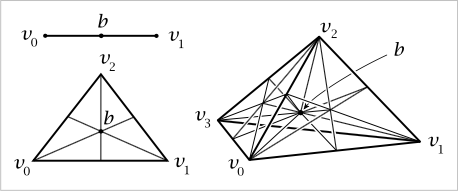
\includegraphics[width=65mm]{Hatcher-barycentric.png}
\caption{copied from Hatcher (120) \label{overflow}}
\end{figure}
\end{enumerate}
\end{definition}

\begin{note}
The vertices of simplices in the barycentric subdivision of $\sigma$ are precisely the barycenters of all the $k$-dimensional faces of $\sigma$ for each $0\leq k\leq n$.
\end{note}


\begin{definition}
The \textit{diameter of $[v_0, \ldots, v_n]$} is $\underset{0\leq i,j\leq n}{\max}\lvert{v_i - v_j}\rvert.$
\end{definition}

\begin{lemma}
If $d$ denotes the diameter of $\sigma\coloneqq  [v_0, \ldots, v_n]$, then the diameter of any $n$-simplex of $B_{\sigma}$ is at most $\frac{nd}{n+1}$.
\end{lemma}
\begin{proof}
For each $i$, we have that
\begin{align*} \lvert{b - v_i}\rvert & = \lvert{\frac{v_0 + \cdots + v_n}{n+1} - v_i}\rvert
\\ & = \lvert{\frac{v_0 + \cdots + v_n}{n+1} - \frac{(n+1)v_i}{n+1}}\rvert
\end{align*}
But $\lvert{v_i - v_i}\rvert=0$, and $\lvert{v_k - v_i}\rvert \leq d$ for each $k$. Hence $ \lvert{b - v_i}\rvert \leq \frac{nd}{n+1}$. We are done by induction on $n$.
\end{proof}


Let $\left(K, \Sigma_K\right)$ be a simplicial complex. Define a new simplicial complex $\left(K' , \Sigma_{K'}\right)$ such that $K' = \Sigma_K$ and $\Sigma^n_{K'} = \{\sigma_0 \subset \sigma_1 \subset \cdots \subset \cdots \subset \sigma_n\}$ wheere each $\sigma_i \in \Sigma_K$.

\medskip

Now, consider a map $\sigma : \Delta^n \to X$, which induces a map $\sigma_{\ast}: C_{\ast}(\Delta^n) \to C_{\ast}(X)$. Let $Y \subset \R^n$ be convex (so that we can apply barycentric subdivision to it.) 

\begin{definition}
For each $k\geq 0$, define the group of \textit{linear chains $LC_k(Y)$} as the free abelian group on the set of linear maps $\Delta^k \to Y$.  For convenience, let $LC_{-1}(Y)\coloneqq  \Z\left[\emptyset\right] \cong \Z$.
\end{definition}

\begin{note}
Any linear chain $\lambda: \Delta^k \to Y$ is determined by the values $w_i \coloneqq  \lambda(v_i)$ where $v_i$ denotes the $i$-th vertex of $\Delta^k$. For each $b\in Y$, we have a group homomorphism $b: LC_k(Y) \to LC_{k+1}(Y)$ given by $[w_0, \ldots, w_k] \mapsto [b, w_0, \ldots, w_k]$. Note that 
\begin{align*} \partial{b[w_0, \ldots, w_k]} & =  \partial{[b, w_0, \ldots, w_k]}
\\ & = [w_0, \ldots, w_k] - \sum_{i=0}^k ({-1})^i[b, w_0, \ldots, \hat{w}_j, \ldots, w_k]
\\ & = [w_0, \ldots, w_k] - b{\partial{[w_0, \ldots, w_k]}}.
\end{align*}
This shows that $\partial{b} + b{\partial} =\1$, so that $b$ is a chain homotopy between $\1$ and and $0$.
\end{note}

\begin{definition}
Let $b_{\lambda}$ denote the image under $\lambda$ of the barycenter of $\Delta^n$. Define the \textit{subdivision map $S: LC_{\ast}(Y) \to LC_{\ast}(Y)$} recursively by
\begin{itemize}
\item $S(\emptyset) = \emptyset$
\item $S\lambda= b_{\lambda}{S(\partial{\lambda})}.$
\end{itemize}
\end{definition}

\begin{note}
If $\lambda$ is an embedding with $\im{\lambda} = \left[w_0, \ldots, w_n\right]$, then $$S\lambda = \left(\text{sum of the }n\text{-simplices (up to sign) in the barycentric subdivision of }\left[w_0, \ldots, w_n\right]\right).$$
\end{note}

\begin{lemma}
$S{\partial} = \partial{S}$.
\end{lemma}
\begin{proof}
We see that $S\restriction_{LC_{-1}(Y)} = \1$. Also, on $LC_0(Y)$ we have that $$S([v]) = b_{[v]}S(\partial{[v]}) =b_{[v]}(\emptyset) =[v] .$$ Thus, $S\restriction_{LC_0(Y)} =\1$ as well. Hence the equation $S{\partial} = \partial{S}$ holds on $LC_0(Y)$. If ${\ast}>0$, then apply the fact that $\partial{b_{\lambda}} + b_{\lambda}{\partial} = \1$ to get
\begin{align*}
 \partial{S\lambda} & = \partial{b_{\lambda}S(\partial{\lambda}})
 \\ & =  (1- b_{\lambda}{\partial})S(\partial{\lambda})
 \\ & = S(\partial{\lambda}) -b_{\lambda}\partial{S(\partial{\lambda})}
 \\ & = S(\partial{\lambda}) - \underbrace{b_{\lambda}S(\partial{\partial{\lambda}})}_{\text{by induction}}
 \\ & = S(\partial{\lambda}) .
\end{align*}
\end{proof}

\medskip

Define $T: LC_n(Y) \to LC_{n+1}(Y)$ a chain homotopy between $\1$ and $S$ recursively by 
\begin{itemize}
\item $T(\emptyset) =0$
\item $T\lambda  = b_{\lambda}(\lambda  - T\partial{\lambda})$.
\end{itemize}
Then the diagram
\[
\begin{tikzcd}
\cdots \arrow[r, "\partial"] & LC_2(Y) \arrow[r, "\partial"] \arrow[d, "S"] & LC_1(Y) \arrow[r, "\partial"] \arrow[d, "S"] \arrow[ld, "T"'] & LC_0(Y) \arrow[r, "\partial"] \arrow[d, "\1"] \arrow[ld, "T"'] & LC_{-1}(Y) \arrow[r, "\partial"] \arrow[d, "\1"] \arrow[d] \arrow[ld, "T"'] & 0 \\
\cdots \arrow[r, "\partial"] & LC_2(Y) \arrow[r, "\partial"]                & LC_1(Y) \arrow[r, "\partial"]                                 & LC_0(Y) \arrow[r, "\partial"]                                  & LC_{-1}(Y) \arrow[r, "\partial"]                                            & 0
\end{tikzcd}
\] commutes.
\begin{lemma}
$\partial{T} + T\partial = \1 - S$.
\end{lemma}
\begin{proof}
When $n= -1$, this is immediate as $T=0$ and $S=\1$. If $n>0$, we compute
\begin{align*}
 \partial{T \lambda} & =  \partial{b_{\lambda}(\lambda  - T\partial{\lambda})}
 \\ & = (\1 - b_{\lambda}{\partial})(\lambda - T{\partial{\lambda}})
 \\ & = \lambda - T\partial{\lambda}- b_{\lambda}(\partial{\lambda} -\partial{T{\partial{\lambda}}})
 \\ & =  \lambda - T\partial{\lambda}- b_{\lambda}(\partial{\lambda} -\underbrace{(\1 -S - T{\partial})}_{\text{by induction}}{\partial{\lambda}})
 \\ & = \lambda - T\partial{\lambda}- b_{\lambda}(\partial{\lambda} - \partial{\lambda} +S{\partial{\lambda}} +T{\partial{\partial}}{\lambda})
 \\ & = \lambda  - T\partial{\lambda}  -b_{\lambda}{S{\partial{\lambda}}}
 \\ & = \lambda  - T\partial{\lambda} -S{\lambda}.
\end{align*}
\end{proof}


\medskip

Now, extend $S$ and $T$ to maps $C_n(X) \to C_n(X)$ and $C_n(X) \to C_{n+1}(X)$, respectively. Let $\sigma \in C_n(X)$.
\begin{notation} $ $
\begin{itemize}
\item $S{\sigma} \equiv \sigma_{\ast}{S{\1_{\Delta^n}}}$.
\item  $T{\sigma} \equiv \sigma_{\ast}{T{\1_{\Delta^n}}}.$
\item $T_m \equiv \sum_{j=0}^{m-1} TS^j $ for any $m\geq 1$.
\end{itemize}
\end{notation}

It's easy to show that $S^m$ is a chain map for any $m\geq 0$ and that $T$ is a chain homotopy between $\1$ and $S$.

\medskip

Moreover, $T_m$ is a homotopy between $\1$ and $S^m$. Indeed,
\begin{align*}
 \partial{T_m} +T_m{\partial} & = \partial{ \sum_{j=0}^{m-1} TS^j} + \sum_{j=0}^{m-1} TS^j{\partial} 
 \\ & = \sum_{j=0}^{m-1} \partial{TS^j} +TS^j{\partial}
 \\ & =  \sum_{j=0}^{m-1} \partial{TS^j} +T\partial{S^j}
 \\ & = \sum_{j=0}^{m-1}(\1 -S)S^j = \1 - S^m.
\end{align*}


\begin{lemma}[Lebesgue covering]
Let $Z$ be a compact metric space. Let $\U =\left\{U_{\alpha}\right\}$ be an open cover of $Z$. Then $\exists \delta >0$ (called a \textit{Lebesgue number for $\U$}) such that for any set $S$ with $\text{diam}(S) < \delta$, $S$ is contained in $U_{\alpha}$ for some $\alpha$.
\end{lemma}

\smallskip

Let $X$ be any space.  Let $\U =\{\mathring{U}_{\alpha}\}$ be a cover of $X$. If $\sigma : \Delta^n \to X$, then consider the open cover $\left\{ \sigma^{-1}(U_{\alpha})\right\} $ of $\Delta^n$. Any $n$-simplex in the $m$-th iteration of the barycentric subdivision of $\Delta^n$ has diameter $$d' \leq \left(\frac{n}{n+1}\right)^md$$ where $d$ denotes the diameter of $\Delta^n$. Then $d'$ is less than a Lebesgue number for $\left\{ \sigma^{-1}(U_{\alpha})\right\}$ when $m$ is large enough, in which case $S^m(\sigma) \in C_n^{\U}(X)$.

Define $m(\sigma)$ as the smallest $m\in \N$ such that $S^m(\sigma) =C_n^{\U}(X)$. Define the map $D: C_n(X) \to  C_{n+1}(X)$ by $D{\sigma} =T_{m(\sigma)}{\sigma}$.


\subsection{Lecture 13}

\begin{lemma} Define the function $\rho : C_{\ast}(X) \to C_{\ast}(X)$ by $\rho = \1 - \partial{D} - D{\partial}$.
\begin{enumerate}
\item $\rho$ is a chain map.
\item $\im{\rho}\subset C_{\ast}^{\U}(X)$. 
\item $\rho$ is a chain homotopy inverse of the inclusion map $\iota : C_{\ast}^{\U}(X) \to C_{\ast}(X)$.
\end{enumerate}
\end{lemma}
\begin{proof} $ $
\begin{enumerate}
\item We compute
\begin{align*}
\partial{\rho{\sigma}} & = \partial(\sigma - \partial{D}{\sigma} - D{\partial}{\sigma})
\\ & = \partial{\sigma} - \partial{D{\partial{\sigma}}}
\\ & = \partial{\sigma} -(\1 -D{\partial} -\rho){\partial{\sigma}}
\\ & = \rho{\partial{\sigma}}.
\end{align*}
\item We compute 
\begin{align*}
\rho(\sigma) & = \sigma - \partial{D}{\sigma} - D{\partial}{\sigma}
\\ & = \sigma - \partial{T_{m(\sigma)}}{\sigma} - D{\partial}{\sigma}
\\ & = S^{m(\sigma)}{\sigma}+T_{m(\sigma)}{\partial{\sigma}} - D{\partial{\sigma}}
\end{align*} since $\partial{T_m} +T_m{\partial} = \1 -S^m$.
Note that $ S^{m(\sigma)}{\sigma} \in C_n^{\U}$ and that the term $T_{m(\sigma)}{\partial{\sigma}} - D{\partial{\sigma}}$ is a linear combination of terms $T_{m(\sigma)}(\partial{\sigma_j}) -T_{m(\sigma_j)}(\sigma_j)$ where each $\sigma_j$  is the restriction of $\sigma$ to a face of $\Delta^n$. Since $m(\sigma_j)\leq m(\sigma)$ for each $\sigma_j$, it follows that $T_{m(\sigma)}{\partial{\sigma}} - D{\partial{\sigma}}$ is a linear combination of terms $TS^i(\sigma_j)$ such that $i\geq m(\sigma_j)$. Each of these terms belongs to $C_n^{\U}$ because $T$ preserves small simplices relative to $\U$.
\item We know that $\partial{D} + D{\partial} =\1 - \iota{\rho}$. Also, if $\sigma$ is small relative to $\U$, then $m(\sigma) =0$, so that $D{\sigma} = 0$. Thus, $\rho{\iota} = \1$.
\end{enumerate}
\end{proof}

\medskip

\begin{proof}[Proof of \cref{excision}]
We prove the equivalent statement expressed in \cref{l25}. Write $X = \mathring{A}\cup \mathring{B}$ with $A,B\subset X$. Let $\U =\{A, B\}$. Note that $C_{\ast}(A)$ is a subcomplex of $C_{\ast}^{\U}(X)$. The diagram
\[
\begin{tikzcd}
0 \arrow[r] & C_{\ast}(A) \arrow[r] \arrow[d, "\text{q-iso}"] & C_{\ast}^{\U}(X) \arrow[r] \arrow[d, "\text{q-iso}"] & C_{\ast}^{\U}(X)/C_{\ast}(A) \arrow[r] \arrow[d] & 0 \\
0 \arrow[r] & C_{\ast}(A) \arrow[r]                          & C_{\ast}(X) \arrow[r]                                & C_{\ast}(X)/C_{\ast}(A) \arrow[r]                & 0
\end{tikzcd}
\] commutes. The five lemma implies that the third vertical arrow is a quasi-isomorphism as well. Finally, note that the inclusion map $\faktor{C_{\ast}(B)}{C_{\ast}(A\cap B)} \to \faktor{C_{\ast}^{\U}(X)}{C_{\ast}(A)}$ is a quasi-isomorphism since both the domain and codomain are free groups with basis the singular $n$-simplices in $B$ that are outside $A$.
\end{proof}

\begin{corollary}[Mayer-Vietoris (MV) sequence]
Let $X= \mathring{A} \cup \mathring{B}$. Then there exists a LES 
\[
\begin{tikzcd}
\cdots \arrow[r] & H_k(A\cap B) \arrow[r] & H_k(A)\oplus H_k(B) \arrow[r] & H_k(X) \arrow[r, "\partial"] & H_{k-1}(A\cap B) \arrow[r] & \cdots
\end{tikzcd}
.\]
\end{corollary}
\begin{proof}
Consider the sequence
\[
\begin{tikzcd}
0 \arrow[r] & C_{\ast}(A\cap B) \arrow[r, "\varphi"] & C_{\ast}(A)\oplus C_{\ast}(B) \arrow[r, "\psi"] & C_{\ast}(X) \arrow[r] & 0
\end{tikzcd}
\] where $\varphi : c \mapsto (c, -c)$ and $\psi : (c_1, c_2) \mapsto c_1 + c_2$. It's easy to check that this is exact, inducing our desired LES.

\medskip

 We can describe the boundary map $\partial : H_k(X) \to H_{k-1}(A\cap B)$. Let $[c] \in H_k(X)$. Then $[c] = [x+y]$ where $x : \Delta^k \to A\subset X$ and $y: \Delta^k \to B\subset X$. Since $\partial(x+y)  =0$, we have that $\partial{x}={-\partial{y}}$. Then $\partial{[c]} =[\partial{x}] = {-[\partial{y}]}$.
\end{proof}

\begin{exmp}
Depict the orientable surface $S_g$ of genus $g$ as 
\begin{figure}[H]
\centering
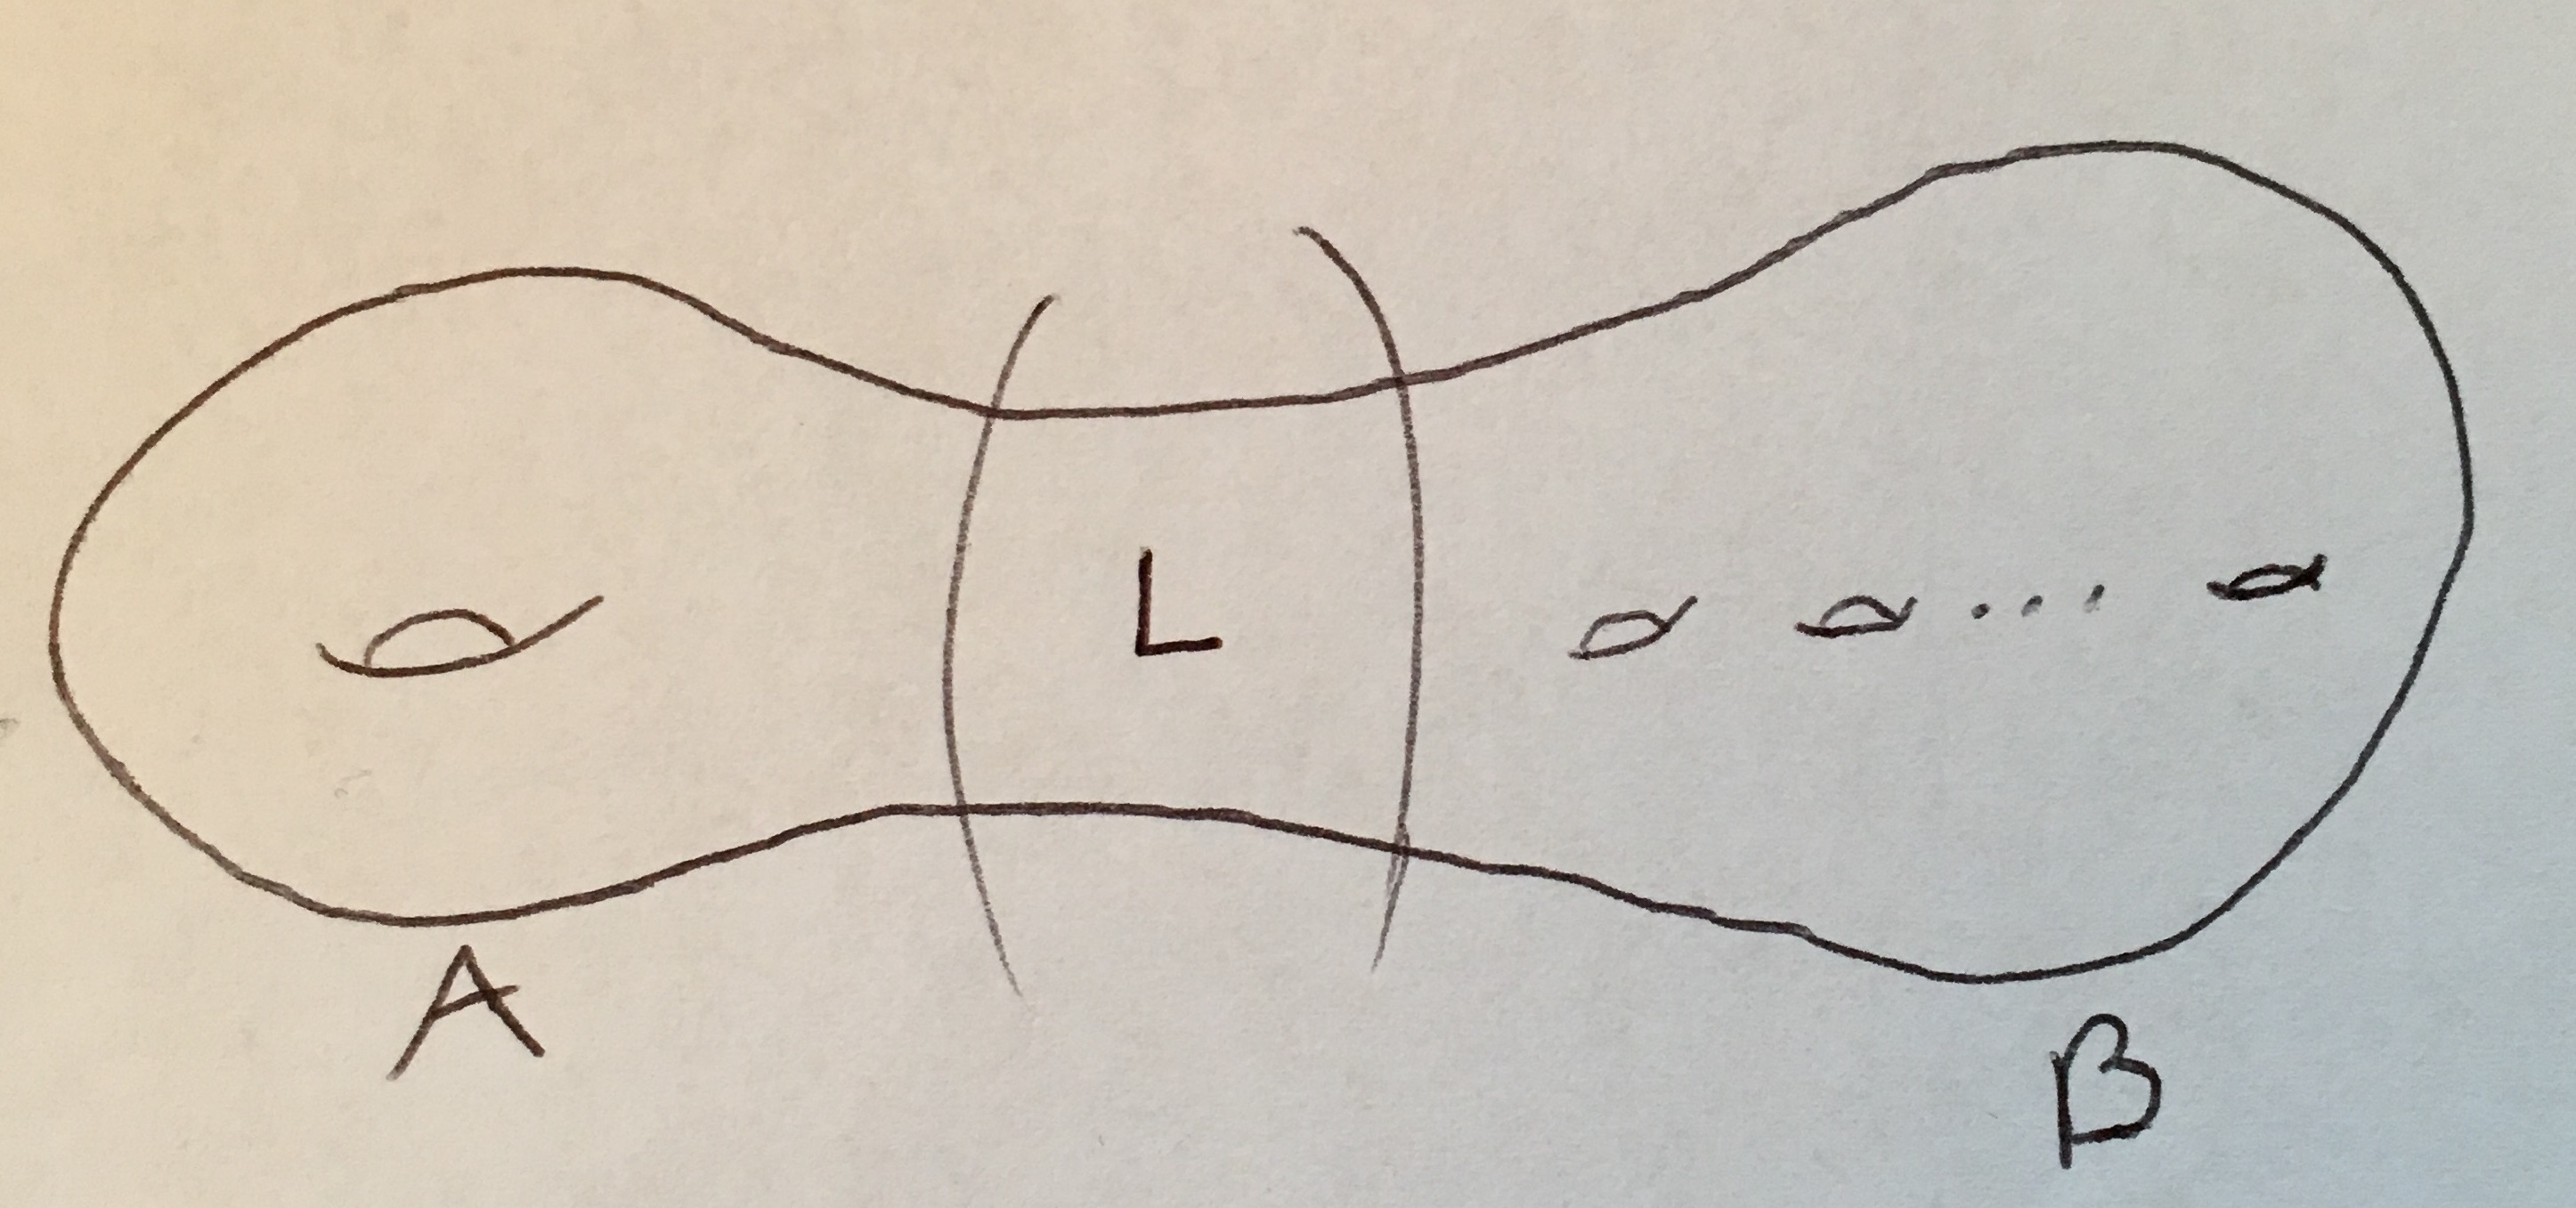
\includegraphics[width=60mm]{S_g-decomposed.jpg}
\end{figure}
so that $A \cap B$ is a cylinder $L$ of finite height. Then $A \cap B = S^1$, $A\simeq S^1 \vee S^1$, and $B\simeq \underbrace{S^1 \vee \cdots \vee S^1}_{2g-2 \text{ copies}}$. We have the MV sequence 
\[ \label{eqn:pseq}
\begin{tikzcd} 
H_2(A) \oplus H_2(B) \arrow[r] & H_2(S_g) \arrow[r]             & H_1(A\cap B) \arrow[r] & H_1(A)\oplus H_1(B) \arrow[r] & H_1(S_g) \arrow[lllld] \\
H_0(A \cap B) \arrow[r]        & H_0(A) \oplus H_0(B) \arrow[r] & H_0(S_g)               &                               &                       
\end{tikzcd} \tag{$\dagger$}
.\] Note that $H_1(A\cap B)$ is generated by the attaching map $\gamma$ of the $2$-cell, which consists of the loop positively traversing $A\cap B$ and the loop negatively traversing $A\cap B$. 
\begin{figure}[H]
\centering
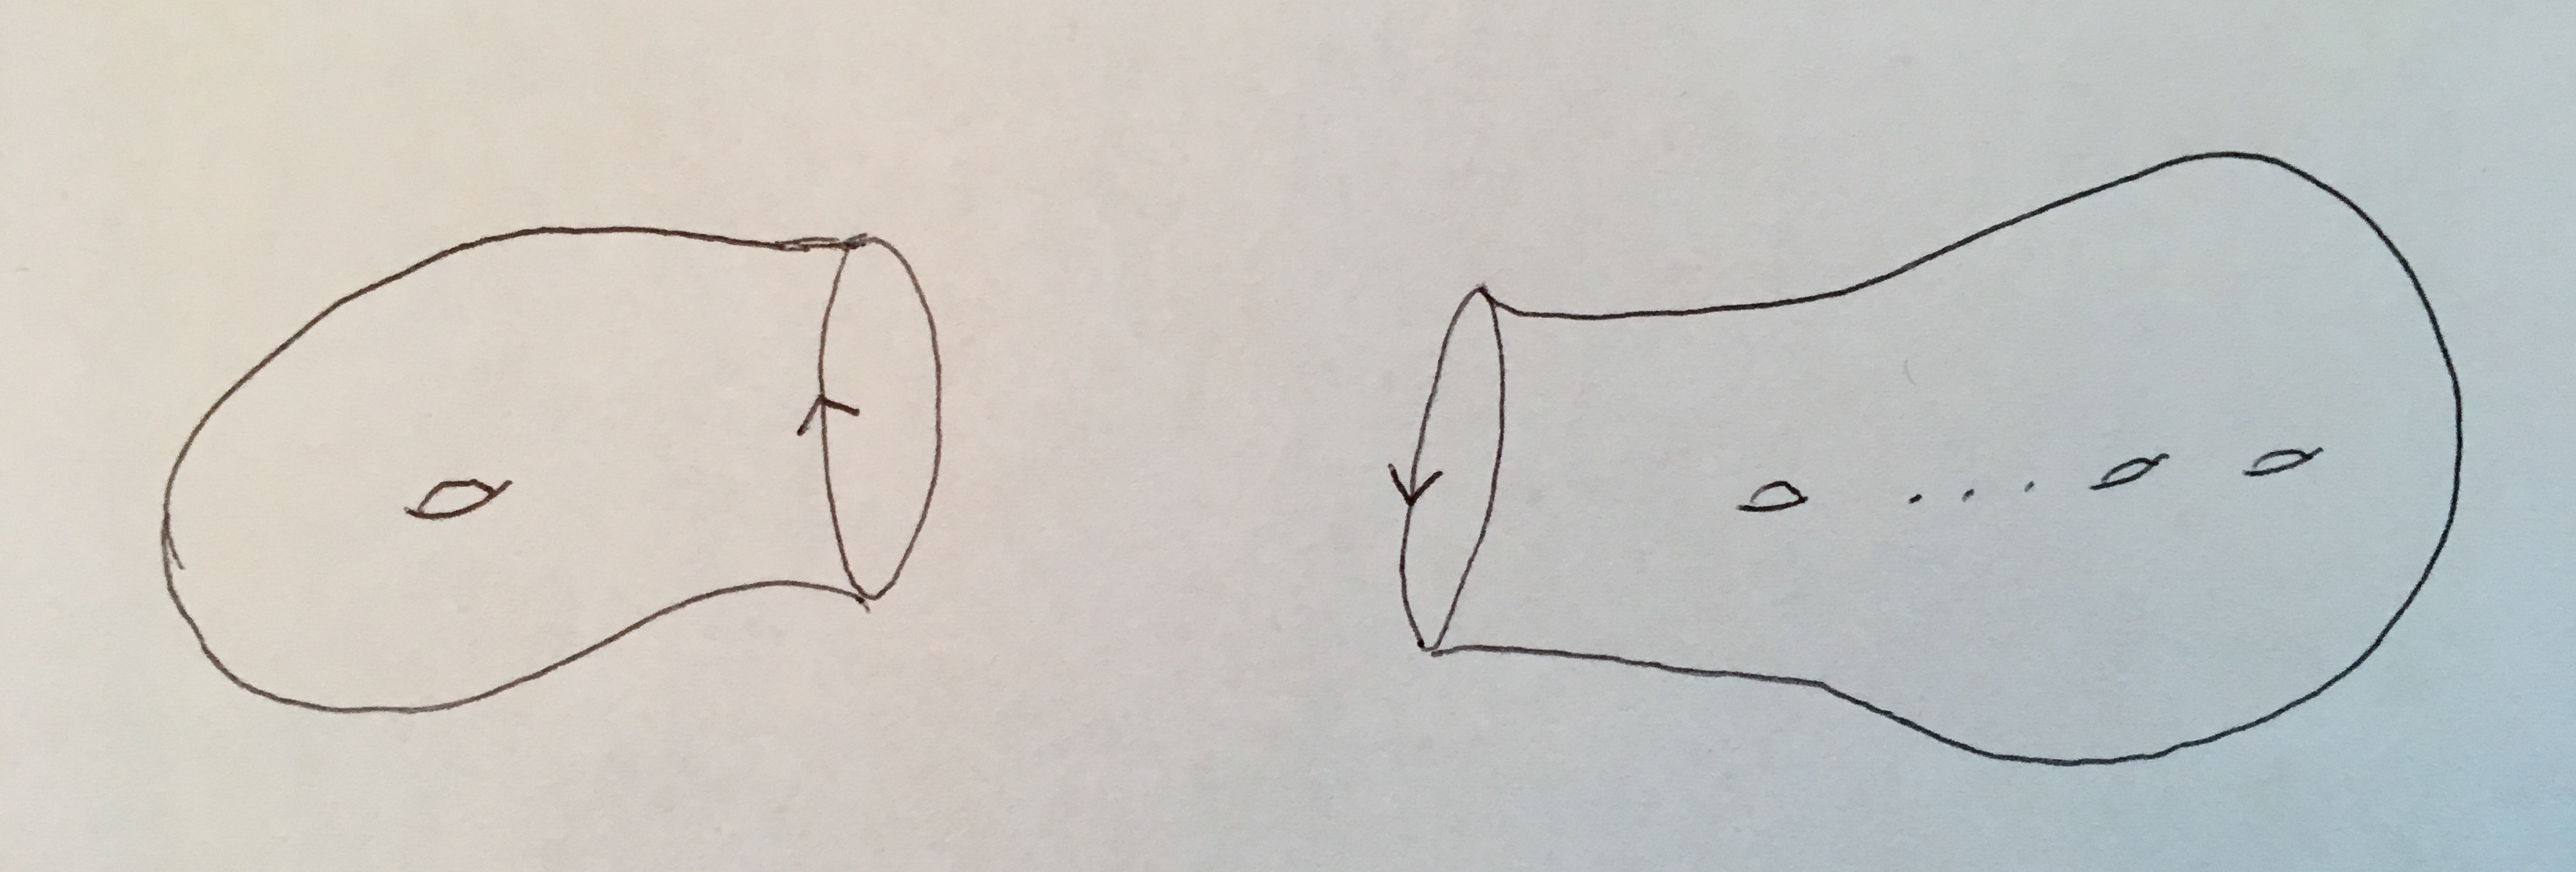
\includegraphics[width=60mm]{S_g-cut.jpg}
\end{figure}
Hence \hl{$\gamma$ is homologous to $0$}. Moreover, both $L$ and $S_g$ are path connected. Hence \eqref{eqn:pseq} becomes 
\[
\begin{tikzcd}
0\oplus 0 \arrow[r]                 & H_2(S_g) \arrow[r]                                  & \Z \arrow[r, "0"] & \Z^2 \oplus \Z^{2g-2} \arrow[r] & H_1(S_g) \arrow[lllld, "0"'] \\
\Z \arrow[r, "{n\mapsto (n, -n)}"'] & \Z \oplus \Z \arrow[r, "{(n,m)\mapsto n+m}"'] & \Z                &                                 &                             
\end{tikzcd}
.\] This implies that $H_1(S_g) \cong \Z^{2g}$ and $H_2(S_g) \cong \Z$.
\end{exmp}

\begin{exmp}
Let $X$ be space and recall the suspension $S{X}= \faktor{X \times I}{\sim}$ of $X$. Let $p_0$ denote the bottom point of the suspension and $p_1$ the top point. We can decompose this space as $$ S{X} = C_+{X} \cup_X C_{-}{X} $$ where $C_+{X} \coloneqq  S{X} \setminus \{p_0\}$ and $C_{-}{X} \coloneqq S{X} \setminus \{p_1\}$. Then both $C_+{X}$ and $C_{-}{X}$ are homotopy equivalent to the cone $C{X}$ and thus are contractible. Note that $ C_+{X} \cap C_{-}{X} \simeq X$. Consider the MV sequence
\[
\begin{tikzcd}
H_k(X) \arrow[r] & H_k(C_+{X})\oplus H_k(C_{-}{X}) \arrow[r] & H_k(S{X}) \arrow[lld] \\
H_{k-1}(X) \arrow[r]                    & H_{k-1}(C_+{X})\oplus H_{k-1}(C_{-}{X})   &                           
\end{tikzcd}
.\] When $k-1>0$, this becomes
\[
\begin{tikzcd}
H_k(X) \arrow[r] & 0\oplus 0 \arrow[r] & H_k(S{X}) \arrow[r] &
H_{k-1}(X) \arrow[r]                    & 0\oplus 0                           
\end{tikzcd},
\] in which case $H_k(S{X}) \cong H_{k-1}(X)$. Moreover, the exact sequence
\[
\begin{tikzcd}
H_1(C_+{X})\oplus H_1(C_{-}{X}) \arrow[r] & H_1(S{X}) \arrow[ld, "0"']             &                \\
H_0(X) \arrow[r]                          & H_0(C_{+}{X})\oplus H_0(C_{-}{X}) \arrow[r] & H_0(S{X})
\end{tikzcd}
\] shows that $H_1(S{X}) =0$.
\end{exmp}

\begin{theorem}[Brouwer's invariance of domain]
Let $U\subset \R^n$ be open and $V\subset \R^m$ be open. If $U \cong V$, then $n=m$.
\end{theorem}
\begin{proof}
Let $x\in U$ and consider $H_{\ast}(U \setminus \{x\})$. By excision, we get $H_{\ast}(U, U \setminus \{x\}) \cong H_{\ast}(\R^n, \R^n \setminus \{x\})$. By \cref{c10}, we also get a LES
\[
\begin{tikzcd}
H_{k}(\R^n \setminus \{x\}) \arrow[r] & H_{k}(\R^n) \arrow[r] & {H_{k}(\R^n, \R^n \setminus \{x\})} \arrow[r] & H_{k-1}(\R^n \setminus \{x\}) \arrow[r] & H_{k -1}(\R^n)
\end{tikzcd}
. \] Let $k\geq 2$. Then $H_k(\R^n, \R^n \setminus \{x\}) \cong H_{k-1}(\R^n \setminus \{x\}) \cong H_{k-1}(S^{n-1}).$ It follows that $$H_k(U, U \setminus \{x\}) \cong \begin{cases} \Z & k=n \\ 0 & k \ne n \end{cases}.$$ If $n >m \geq 1$, then $H_n(U, U \setminus \{x\}) \cong \Z$ whereas $H_n(V, V \setminus \{x'\}) \cong 0$ for any $x' \in V$. In this case, $U \not \cong V$.
\end{proof}

\subsection{Lecture 14}

Recall that $H_n(D^n, S^{n-1}) \cong H_n(S^n) \cong \Z$. Note that $(D^n, S^{n-1}) \cong (\Delta^n, \partial{\Delta^n})$ and that $i_n : \Delta^n \hookrightarrow \Delta^n$ is a cycle in $C_n(\Delta^n, \partial{\Delta^n})$. We

\begin{lemma}
$i_n$ generates $H_n(\Delta^n, \partial{\Delta^n})$.
\end{lemma}
\begin{proof}
We do induction on $n$. For the base case, it is obvious that $H_0(\Delta^0, \underbrace{\partial{\Delta^0}}_{\emptyset})$ is generated by $i_0$. Let the subspace $\wedge \subset \partial{\Delta^n}$ consist of all but one of the faces of $\partial{\Delta^n}$. Consider the triple $(\Delta^n, \partial{\Delta^n}, \wedge)$. This induces the LES
\[
\begin{tikzcd}
{H_n(\partial{\Delta^n, \wedge})} \arrow[r] & {H_n(\Delta^n, \wedge)} \arrow[r] & {H_n(\Delta^n, \partial{\Delta^n)}} \arrow[r] & {H_{n-1}(\partial{\Delta^n}, \wedge)} \arrow[r] & {H_{n-1}(\Delta^n, \wedge)}
\end{tikzcd}
.\] Since \hl{$H_n(\Delta^n, \wedge) =0 = H_{n-1}(\Delta^n, \wedge)$}, it follows that $\alpha: H_n(\Delta^n, \partial{\Delta^n)} \overset{\cong}{\longrightarrow}  H_{n-1}(\partial{\Delta^n}, \wedge)$. Moreover, obtain an isomorphism $\beta: H_{n-1}(\Delta^{n-1}, \partial{\Delta^{n-1}}) \overset{\cong}{\longrightarrow} H_{n-1}(\partial{\Delta^n}, \wedge)$ from the homeomorphism of pairs $(\Delta^{n-1}, \partial{\Delta^{n-1}}) \to (\partial{\Delta^n}, \wedge)$ that maps $\Delta^{n-1}$ to the face missing in $\wedge$. The inductive step now holds because \hl{$\alpha{i_n} = \partial{i_n}= \pm \beta{i_{n-1}}$}.
\end{proof}

\begin{corollary}
Consider the sphere $$S^n = D^n \cup_{S^{n-1}} D^n= \Delta^n \cup_{\partial{\Delta^n}}\Delta^n$$ and the inclusion maps 
\begin{align*}
& \Delta^n_1 :\Delta^n \to \text{first}(\Delta^n)
\\ &  \Delta^n_2 :\Delta^n \to \text{second}(\Delta^n).
\end{align*} Then $\Delta^n_1 - \Delta^n_2$ is a cycle. We claim that $\Delta_1^n -\Delta_2^n$ generates $\widetilde{H}_n(S^n)$.
\end{corollary}
\begin{proof}
We have that $\widetilde{H}_n(S^n) \overset{\cong}{\longrightarrow} H_n(S^n, \im{\partial_2^n}) \overset{\cong}{\longleftarrow} H_n(\im{\Delta^n_1}, \partial{\im{\Delta_1^n}})$ where $\Delta_1^n -\Delta_2^n \mapsto \Delta^n_1 \mapsfrom i_n$.
\end{proof}

\smallskip

Let $f: S^n \to S^n$ be a map, inducing the endomorphism $f_{\ast} : \widetilde{H}_n(S^n) \cong \Z \to \widetilde{H}_n(S^n) \cong \Z$. Then $f_{\ast}(g) = \alpha g$ for some $\alpha \in \Z$. 

\begin{definition}
We call such an $\alpha$ the \textit{degree of $f$}, written as $\deg{f}$.
\end{definition}

\begin{prop} $ $
\begin{enumerate}
\item $\deg{\1_{S^n}}=1$.
\item If $f: S^n \to S^n$ is not surjective, then $\deg{f} = 0$.
\begin{proof}
Let $x\in S^n \setminus \im{f}$. Since $S^n \setminus \{x\} \cong \R^n$, we have that 
\[
\begin{tikzcd}
\widetilde{H}_n(S^n) \arrow[r, "f_{\ast}"] \arrow[d] & \widetilde{H}_n(S^n) \\
\underbrace{\widetilde{H}_n(S^n \setminus \{x\})}_{0} \arrow[ru]      &                     
\end{tikzcd}
\]
\end{proof}
\item If $f \simeq g$, then $\deg{f} = \deg{g}$ since $f_{\ast} = g_{\ast}$.
\item By functorality, we get $\deg{fg}= \deg{f}\cdot \deg{g}$.
\begin{corollary}
If $f$ is a homotopy equivalence, then $\deg{f}= \pm 1$.
\end{corollary}
\item Define the map $i_k : S^n \to S^n$ by $(x_0, \ldots, x_n) \mapsto (x_0, \ldots, -x_k, \ldots, x_n)$. Then $\deg{i_k} = {-1}$.
\begin{proof}
Recall that $\Delta_1^n -\Delta_2^n$ generates $\widetilde{H}_n(S^n)$. Situate things so that $\partial{\Delta_1^n} = \partial{\Delta_2^n}$ is in the hyperplane $x_k=0$. Then $i_k$ fixes both $\partial{\Delta_1^n}$ and $\partial{\Delta_2^n}$ and interchanges the two hemispheres. Hence $i_k(\Delta_1^n -\Delta_2^n)= \Delta_2^n- \Delta_1^n $.
\end{proof}
\item Let $i: S^n \to S^n$ be the antipodal map. Then $\deg{i} = ({-1})^{n+1}$ since $i= i_0 \circ i_1 \circ \cdots \circ i_n$.
\item Suppose that $f: S^n \to S^n$ has no fixed point. Then $\deg{f}= ({-1})^{n+1}$.
\begin{proof}
If $f(x) \ne x$ for every $x\in S^n$, then the line segment $(1-t)f(x) - tx$ never passes through the origin. Therefore, the maps $$H_t = \frac{ (1-t)f(x)-tx  }{\lvert{(1-t)f(x) -tx}\rvert     }$$ define a homotopy between $f$ and the antipodal map $i$.
\end{proof}
\end{enumerate}
\end{prop}

\smallskip

Let $f: S^n \to S^n$ and $x\in S^n$ such that $f^{-1}(x)= \{x_1, \ldots, x_m\}$. Let $U_1, \ldots, U_m$ be pairwise disjoint neighborhoods of $x_1, \ldots, x_m$, respectively, where we can find a neighborhood $V$ of $x$ such that each $U_i$ is mapped by $f$ into $V$. Then $f(U_i \setminus \{x_i\}) \subset V \setminus \{x\}$. For each $i=1, \ldots, m$, we have a commutative diagram
\[
\begin{tikzcd}
                                 & {H_n(U_i, U_i \setminus \{x_i\})} \arrow[ld, "\cong"'] \arrow[d, "k_i"] \arrow[r, "f_{\ast}"] & {H_n(V, V\setminus \{x\})} \arrow[d, "\cong"] \\
{H_n(S^n, S^n\setminus \{x_i\})} & {H_n(S^n, S^n \setminus \{f^{-1}(x)\})} \arrow[r, "f_{\ast}"] \arrow[l, "p_i"]                & {H_n(S^n, S^n \setminus \{x\})}               \\
                                 & H_n(S^n) \arrow[lu, "\cong"] \arrow[u, "j"'] \arrow[r, "f_{\ast}"] \arrow[u]                  & H_n(S^n) \arrow[u, "\cong"']                 
\end{tikzcd}
\] where the two upper isomorphisms come from excision and the two lower isomorphisms come from the LES of \cref{c10}. Therefore, the homomorphism $f_{\ast} : H_n(U_i, U_i \setminus \{x_i\}) \to H_n(V, V\setminus \{x\})$ can be viewed as a homomorphism $f_{\ast} : \Z \to \Z$, so that $f_{\ast}(g) = \alpha g$ for some $\alpha \in \Z$. We call $\alpha$ the \textit{local degree of $f$ at $x$}, written as $\deg_{x_i}{f}$.


\begin{lemma}
$\deg{f}  = \sum_{i=1}^m \deg_{x_i}{f}$.
\end{lemma}
\begin{proof}
By excision, we get $$H_n(S^n, S^n \setminus f^{-1}(x)) \cong H_n\left(\coprod_{i=1}^m U_i,  \coprod_{i=1}^m U_i \setminus \{x_i\}\right) \cong \bigoplus_{i=1}^m H_n(U_i, U_i \setminus \{x_i\}).$$ \hl{By the naturality of excision}, we see that $k_i$ corresponds to the $i$-th inclusion map and that $p_i$ corresponds to the $i$-th projection map. By a straightforward diagram chase, we are done.
\end{proof}

\subsection{Lecture 15}

\begin{lemma}
Let $X$ be a CW-complex with skeleta $X^n$.
\begin{enumerate}
\item $H_k(X^n, X^{n-1}) =\begin{cases}  0 & k\ne n \\ \Z\left[n\text{-cells of } X\right] & k= n  \end{cases}$.
\item $H_k(X^n) =0$ when $k>n\geq 0$. In particular, $H_k(X) = 0$ when $k> \dim{X}$.
\item The inclusion $i: X^n \to X$ induces an isomorphism $i_{\ast} : H_k(X^n) \overset{\cong}{\longrightarrow} H_k(X)$ when $k<n$.
\end{enumerate}
\end{lemma}
\begin{proof} $ $
\begin{enumerate}
\item Since $(X^n, X^{n-1})$ is a good pair, we see that $$H_k(X^n, X^{n-1}) \cong \widetilde{H}_k(X^n/X^{n-1}) \cong \widetilde{H}_k \left(\bigvee_{n\text{-cells of X}} S^n \right).$$
\item Assume that $k>n$. We have a LES 
\[
\begin{tikzcd}
\cdots \arrow[r] & {\underbrace{H_{k+1}(X^n, X^{n-1})}_{0}} \arrow[r] & H_k(X^{n-1}) \arrow[r] & H_k(X^n) \arrow[r] & {\underbrace{H_k(X^n, X^{n-1})}_{0}} \arrow[r] & \cdots
\end{tikzcd}
.\] Hence the map $H_k(X^{n-1}) \to H_k(X^n)$ is an isomorphism. From this we get a chain of isomorphisms
\[
\begin{tikzcd}
H_k(X^0) \arrow[r, "\cong"] & H_k(X^1) \arrow[r, "\cong"] & \cdots \arrow[r, "\cong"] & H_k(X^{k-1})
\end{tikzcd}
\] induced by inclusion.  We are done because $H_k(X^0)=0$.
\item If $k<n$, then the LES from part 2 produces a chain of isomorphisms 
\[
H_k(X^n) \cong H_k(X^{n+1}) \cong H_k(X^{n+2}) \cong \cdots
.\] Any $c \in C_k(X)$ has compact image and thus intersects at most finitely many cells of $X$. Thus, $[c] \in H_k(X^m)$ for some $m>k$. By our chain of isomorphisms, it follows that $[c] = [\tilde{c}]$ for some $[\tilde{c}]\in H_k(X^n)$. This proves that $i_{\ast}$ is surjective. Moreover, if $[ic] = 0$ in $H_k(X)$, then there exists $m >n$ such that $c = \partial{\tilde{c}}$ for some chain $\tilde{c}$ in $X^m$. By out chain of isomorphism, it follows that $[c]=0$ in $H_k(X^n)$. This proves that $i_{\ast}$ is surjective. 
\end{enumerate}
\end{proof}

\begin{definition}[Cellular homology]
Let $X$ be a CW-complex. Consider the three pairs 
\begin{gather*}
\left(X^{n+1}, X^n\right)
\\ \left(X^n, X^{n-1}\right)
\\ \left(X^{n-1}, X^{n-2}\right).
\end{gather*} We have a commutative diagram
\[
\begin{tikzcd}
                 & 0                                                                        &                                                                &                                        &        \\
0 \arrow[rd]     & {\quad \quad H_n(X^{n+1})\cong H_n(X)} \arrow[u]                                       &                                                                &                                        &        \\
                 & H_n(X^n) \arrow[rd, "j_n"] \arrow[u]                                     &                                                                &                                        &        \\
\cdots \arrow[r] & {H_{n+1}(X^{n+1}, X^n)} \arrow[r, "d_{n+1}"] \arrow[u, "\partial_{n+1}"] & {H_n(X^n, X^{n-1})} \arrow[rd, "\partial_n"'] \arrow[r, "d_n"] & {H_{n-1}(X^{n-1}, X^{n-2})} \arrow[r]  & \cdots \\
                 & \vdots \arrow[u]                                                         &                                                                & H_{n-1}(X^{n-1}) \arrow[u, "j_{n-1}"'] &        \\
                 &                                                                          &                                                                & 0 \arrow[u]                            &       
\end{tikzcd}
\] where $d_n \coloneqq  j_{n-1}{\partial_n}$, called a \textit{cellular boundary map}. It is clear that $d^2 =0$, so that the horizontal row is a chain complex $\left(H_n(X^n, X^{n-1}), d_n\right)$. This gives rise to the \textit{cellular homology of $X$}, written as $H_{\ast}^{\cw}(X)$.
\end{definition}

\begin{theorem}
For any CW-complex $X$, $H_n^{\cw}(X) \cong H_n(X)$.
\end{theorem}
\begin{proof}
Note that $H_n(X) \cong \faktor{H_n(X^n)}{\im{\partial_{n+1}}}$. Since $j_n$ is injective, we see that $$\im{d_{n+1}} = \im{j_n{\partial_{n+1}}} = j_n(\im{\partial_{n+1}}) \cong \im{\partial_{n+1}}$$. Since $j_{n-1}$ is also injective, we get $$H_n(X^n) \cong j_n(H_n(X^n)) = \im{j_n} = \ker{\partial_n} = \ker{d_n}.$$ Thus, $j_n : H_n(X^n) \overset{\cong}{\longrightarrow} \ker{d_n}$ such that $j_n(\im{\partial_{n+1}}) = \im{d_{n+1}}$, which implies that $$ \faktor{H_n(X^n)}{\im{\partial_{n+1}}} \cong \faktor{\ker{d_n}}{\im{d_{n+1}}} = H_n^{\cw}(X).$$
\end{proof}

\begin{corollary}\label{c19}
If $X$ is connected and contains only one $0$-cell, then $d_1 : H_1(X^1, X^0) \to H_0(X^0)$ is the zero map.
\end{corollary}

\begin{corollary}
If $X$ is a CW-complex with no $n$-cells, then $H_n(X) =0$.
\end{corollary}

\begin{exmp}
Recall that $\CP^n = e^0 \cup e^2 \cup e^4 \cup \cdots \cup e^{2n}$. Hence each map $d_i =0$, so that $H_k^{\cw}(\CP^n)\cong H_k(X^k, X^{k-1})$. Therefore, $$H_k(\CP^n) = \begin{cases}  \Z & k \text{ even and } k\leq 2n  \\ 0 & \text{otherwise}  \end{cases}.$$
\end{exmp}

\medskip

Now, let $X$ be a CW-complex and $n>1$. Let $d_{\alpha \beta}$ denote the degree of the composite $$S_{\alpha}^{n-1} \overset{\varphi_{\alpha}}{\longrightarrow} X^{n-1} \overset{q_{\beta}q}{\longrightarrow} S_{\beta}^{n-1}$$ where $\varphi_{\alpha}$ denotes the attaching map of $e_{\alpha}^n$, $q: X^{n-1} \to \faktor{X^{n-1}}{X^{n-2}}$ denotes the quotient map, and $q_{\beta} : \faktor{X^{n-1}}{X^{n-2}} \to S_{\beta}^{n-1}$ denotes the map collapsing $X^{n-1} \setminus e_{\beta}^{n-1}$ to a point. 

\begin{prop}[Cellular boundary formula]
$ d_n(e_{\alpha}^n) = \sum_{\beta} d_{\alpha{\beta}}e_{\beta}^{n-1} .$
\end{prop}

 Note that this summation contains only finitely many terms since $\varphi_{\alpha}$ has compact image and thus intersects only finitely cells $e_{\beta}^{n-1}$.

\begin{proof}
Let $\Delta_{\alpha{\beta}}\coloneqq  q_{\beta}q \varphi_{\alpha}$. Then we have a commutative diagram
\[
\begin{tikzcd}
{H_n(D^n_{\alpha}, \partial{D_{\alpha}^n})} \arrow[d, "\Phi_{\alpha{\ast}}"] \arrow[r, "\partial"] & \widetilde{H}_{n-1}(\partial{D_{\alpha}^n}) \arrow[r, "\Delta_{\alpha{\beta}}{\ast}"] \arrow[d, "\varphi_{\alpha{\ast}}"] & \widetilde{H}_{n-1}(S_{\beta}^{n-1})                                                  \\
{H_n(X^n, X^{n-1})} \arrow[rd, "d_n"'] \arrow[r, "\partial_n"]                                     & \widetilde{H}_{n-1}(X^{n-1}) \arrow[r, "q_{\ast}"] \arrow[d, "j_{n-1}"]                                                   & \widetilde{H}_{n-1}(X^{n-1}/X^{n-2}) \arrow[u, "q_{\beta{\ast}}"'] \arrow[d, "\cong"] \\
                                                                                                   & {H_{n-1}(X^{n-1}, X^{n-2})} \arrow[r, "\cong"]                                                                            & {H_{n-1}(X^{n-1}/X^{n-2}, X^{n-2}/X^{n-2})}                                          
\end{tikzcd}
.\] The map $\Phi_{\alpha{\beta}{\ast}}$ sends any generator $[D_{\alpha}^n]$ to the generator $e_{\alpha}^n$. From this we se that $$  d_n(e_{\alpha}^n) = j_{n-1}\varphi_{\alpha{\ast}}\partial{[D_{\alpha}^n]}  .$$ Also, the map $q_{\beta{\ast}}$ is precisely the projection map onto the copy of $\Z$ corresponding to the basis element $e_{\beta}^{n-1}$. A simple diagram chase yields our desired formula. 
\end{proof}

\begin{exmp} $ $
\begin{enumerate}
\item The closed orientable surface $S_g$ of genus $g$ has one $0$-cell, $2g$ $1$-cells, and one $2$-cell. Thus, we get the cellular chain complex 
\[
\begin{tikzcd}
0 \arrow[r] & \Z \arrow[r, "d_2"] & \Z^{2g} \arrow[r, "d_1"] & \Z \arrow[r] & 0
\end{tikzcd}
.\] We know that $d_1=0$ because $S_g$ is connected and has exactly one $0$-cell. Moreover, the maps $\Delta_{\alpha{\beta}}$ are homotopic to constant maps, which implies that $d_2 =0$. It follows that $$  H_n(S_g) \cong \begin{cases}  \Z & n\in \{0,2\} \\ \Z^{2g} & n =1 \\ 0 & \text{otherwise} \end{cases}  .$$
\item Recall that $\RP^n = e^0 \cup e^1 \cup \cdots \cup e^n$ with attaching maps the two-sheeted covering projections $\varphi : S^{k-1} \to \RP^{k-1}$. If $q : \RP^{k-1} \to \RP^{k-1}/\RP^{k-2} = S^{k-1}$ denotes the quotient map, then the composite $q{\varphi}$ is a homeomorphism when restricted to each of the two components of $S^{k-1} \setminus S^{k-2}$, one being the identity and the other being the antipodal map. In particular, these two homeomorphisms are obtained from each other by precomposing with the antipodal map $S^{k-1} \to S^{k-1}$, which has degree $({-1})^k$. Therefore, $\deg{q\varphi} = \deg(\1)+\deg({-\1}) = 1+({-1})^k$ by our local-degree formula. It follows that
\[
\begin{tikzcd}
0 \arrow[r] & \Z \arrow[r, "2"] & \Z \arrow[r, "0"] & \cdots \arrow[r, "2"] & \Z \arrow[r, "0"] & \Z \arrow[r, "2"] & \Z \arrow[r, "0"] & \Z \arrow[r] & 0 & n \text{ even} \\
0 \arrow[r] & \Z \arrow[r, "0"] & \Z \arrow[r, "2"] & \cdots \arrow[r, "2"] & \Z \arrow[r, "0"] & \Z \arrow[r, "2"] & \Z \arrow[r, "0"] & \Z \arrow[r] & 0 & n \text{ odd}.
\end{tikzcd}
\] Hence $$ H_k(\RP^n) \cong \begin{cases}   \Z & k=0 \text{ or } k=n \text{ odd} \\ \Z/2 & 0< k<n, \ k \text{ odd}  \\ 0 & \text{otherwise} \end{cases}  .$$
\item Let $m>1$ be an integer and $l_1, \ldots, l_n$ be relatively prime to $m$. Let $\rho$ be the action of $\Z/m$ on $S^{2n-1} \subset \C$ generated by the homeomorphism $$(z_1, \ldots, z_n) \mapsto (e^{\frac{2\pi il_1}{m}}z_1, \ldots, e^{\frac{2\pi il_n}{m}}z_n).$$  The orbit space $S^{2n-1}/\Z_m$ is called the \textit{lens space $L\coloneqq  L_m(l_1, \ldots, l_n)$}. Note that the projection $S^{2n-1} \to L$ is a covering space since $\rho$ is free.
\end{enumerate}

\end{exmp}

\smallskip

Let $G$ be a finitely generated abelian group. We can write $G$ uniquely as  $\Z^m \times T_1 \times \cdots \times T_s$ where each $T_i$ is a  finite cyclic group. Let $\rnk{G} = m$.

\begin{definition}[Euler characteristic]
 Let $X$ be a space whose singular chain complex is finite. The \textit{Euler characteristic $\chi(X)$ of $X$} is $ \sum_n({-1})^n\rnk{H_n(X)}$, which is a finite sum by \cref{c19}.
\end{definition}

\begin{note}
Let $(C_{\ast}, d)$ be a chain complex of finitely generated abelian groups. The induced homology groups $H_{\ast}$ are finitely generated abelian groups as well. 
\end{note}

\begin{exercise}
Show that if $0 \to A \to B \to C \to 0$ is an exact sequence of finitely generated abelian groups, then $\rnk{B}= \rnk{A} + \rnk{C}$.
\end{exercise}

\begin{lemma}
Let $(C_{\ast}(X), d)$ be a finite singular chain complex. Then $\chi(X) =\sum_n ({-1})^n\rnk{C_n}$.
\end{lemma}
\begin{proof}
We can write out chain complex as
\[\begin{tikzcd}
0 \arrow[r] & C_k \arrow[r, "d_k"] & C_{k-1} \arrow[r, "d_{k-1}"] & \cdots \arrow[r] & C_1 \arrow[r, "d_1"] & C_0 \arrow[r] & 0
\end{tikzcd}
.\] We have short exact sequences $0 \to Z_n \to C_n \to B_{n-1} \to 0$ and $0 \to B_n \to Z_n \to H_n \to 0$. This shows that $\rnk{C_n}= \rnk{Z_n} +\rnk{B_{n-1}}$ and $\rnk{Z_n} = \rnk{B_n} + \rnk{H_n}$. It follows that $$\rnk{C_n}=  \rnk{B_n} + \rnk{H_n}  +\rnk{B_{n-1}}  .  $$ Hence $ \sum_n({-1})^n\rnk{C_n(X)} =  \sum_n({-1})^n\rnk{H_n(X)}$.
\end{proof}

\begin{corollary}
 Let $X$ be a finite CW-complex. Then $$\chi(X) = \sum_{n} ({-1})^nc_n$$ where $c_n$ denotes the number of $n$-cells of $X$.
\end{corollary}

\subsection{Lecture 16}

\begin{theorem}
Let $X$ be a path connected space. There exists a surjective map $h: \pi_1(X) \to H_1(X)$ with $\ker{h} = [\pi_1(X), \pi_1(X)]$. In this case, $$\pi_1(X)_{ab} \cong H_1(X).$$
\end{theorem}
\begin{proof}
Define $h: \pi_1(X) \to H_1(X)$ by $\gamma \mapsto \sigma_{\gamma}$ where $\sigma_{\gamma}(t) \equiv \gamma(t)$.  
\end{proof}

\begin{exmp}
We have surjective maps $\pi_1(S^1 \vee S^1) \cong \F_2 \to H_1(S^1 \vee S^1) \cong \Z^2$ and $\pi_1(S_g) \to H_1(S_g) \cong \Z^{2g}$.
\end{exmp}

\medskip


\begin{definition}
Let $R$ be a (unital) ring. Let $M$ be an $R$-module and $N$ be a right $R$-module. The \textit{tensor product $\left(N \otimes_R M, \psi\right)$} consists of an $R$-module $N \otimes_R M$ and a $R$-bilinear map $\psi : N \times M \to N \otimes_R M$ such that for any $R$-bilinear map $f: N \times M \to F$, there is a unique $R$-linear map $g : N \otimes_R M \to F$ such that $g{\psi} = f$.
\end{definition}

\begin{prop} $ $
\begin{enumerate}
\item $N \otimes_R R \cong N$.
\item $\Z^n \otimes_{\Z} \Z^m \cong \Z^{nm}$.
\item $\Z/n \otimes_{\Z} \Z/m \cong \Z/ (n,m)$.
\end{enumerate}
\end{prop}

\begin{definition}[Homology with coefficients]
Let $G$ be an abelian group and $X$ be a space.  Define $(C_{\ast}(X; G), \partial)$ as $(C_{\ast} \otimes_{\Z} G, \partial \otimes \1) $ and $H_{\ast}(X;G)$ as $H_{\ast}(C_{\ast}(X;G))$.
\end{definition}

\begin{note}
It it \textit{not} the case that if $C_{\ast}$ is a chain complex, then $H_{\ast}(C_{\ast} \otimes G) \cong H_{\ast}(C_{\ast}) \otimes G$.
\end{note}


\medskip

Let $M$ be an $R$-module. Consider the functor $N \mapsto N \otimes_R M$ from $R^{\op}{-}\mathbf{Mod}$ to $\mathbf{Ab}$. This is right exact and thus has \textit{left derived functors}  denoted by $\tor_i^R({-}, M)$.  Specifically, from any projective resolution $\cdots \to P^2 \to P^2 \to P^0 \to N\to 0$ in $R^{\op}{-}\mathbf{Mod}$, construct $C_{\ast}$ the chain complex $$\cdots  \to P^2 \otimes_R M\to  P^1 \otimes_R M\to  P^0 \otimes_R M  \to 0.$$ Then $\tor_i^R(N, M) = H_i(C_{\ast}).$
\begin{note}
Our definition of $\tor_i^{R}$ is independent of the choice of projective resolution. 
\end{note}

\smallskip

Consider a functor $F$ from $\mathbf{Top}$. It may be that $FX$ depends on more than the homotopy type of $X$. To ``extend" $F$ to the homotopy category, we replace $X$ by an equivalent cofibrant space or CW-complex. Since projective modules are precisely the cofibrant spaces in $\mathbf{Mod}$, we see that $$ \cdots \to P^1 \to P^0$$ is a \textit{cofibrant replacement} of $N$. This is why we remove $N$ when constructing our new chain complex $C_{\ast}$ above.

\begin{exmp} $ $
\begin{enumerate}
\item We have a free resolution $0 \to \Z \overset{n}{\longrightarrow} \Z \to \Z/n \to 0$ of $\Z/n$ over $\Z$, from which we form the complex $$ \Z \otimes \Z \overset{n \otimes \1}{\longrightarrow} \Z \otimes \Z  \to 0   .$$ This is precisely $ \Z \overset{n}{\longrightarrow} \Z \to 0$. Hence $$\tor_i^{\Z}(\Z/n, \Z) \cong  \begin{cases} \Z/n & i =0 \\ 0 & i >0 \end{cases} .$$
\item We have a trivial free resolution $0 \to \Z \to \Z \to 0$ of $\Z$ over $\Z$. From this we form the complex $$ 0 \to \Z \otimes \Z /n  \to 0, $$ which becomes $0 \to \Z/n \to 0$. Hence $$\tor_i^{\Z}(\Z, \Z/n) \cong  \begin{cases} \Z/n & i =0 \\ 0 & i >0 \end{cases} .$$
\item We have a free resolution $0 \to \Z \overset{n}{\longrightarrow} \Z \to \Z/n \to 0$ of $\Z/n$ over $\Z$, from which we form the complex $$ \Z \otimes \Z/m \overset{n \otimes \1}{\longrightarrow} \Z \otimes \Z/m  \to 0   .$$ This is precisely $ \Z/m \overset{n}{\longrightarrow} \Z/m \to 0$. Hence $$\tor^{\Z}_i(\Z/n, \Z/m) \cong \begin{cases} \ker( \Z/m \overset{n}{\longrightarrow} \Z/m) \cong  \Z/(n,m) & i =1 \\ 0 & i \ne 1 \end{cases}.$$
\end{enumerate}
\end{exmp}

\smallskip

Suppose that $(C_{\ast}, \partial)$ is a chain complex and that $0 \to P^1 \to P^0 \to H \to 0$ is a projective resolution. For each $n\in \N$, we get a (non-canonical) split short exact sequence $$0 \to H_n(X) \otimes G \to H_n(X; G) \to \tor_1(H_{n-1}(X), G) \to 0    ,$$ called the \textit{universal coefficient sequence (for homology)}. Therefore, $$H_n(X; G) \cong (H_n(X) \otimes G)  \oplus  \tor_1(H_{n-1}(X), G).$$


\begin{exmp}
Let $X= \RP^n$ and $G= \Z/2$. By the universal coefficient sequence, it is straightforward to show that $$H_n(\RP^n; \Z/2) \cong \Z/2 $$ for every $n$. For example, we have that
\begin{align*}
H_1(\RP^n, \Z/2) & \cong H_1(\RP^n; \Z/2) \cong (H_1(X) \otimes \Z/2)  \oplus  \tor_1(H_0(\RP^n), \Z/2)
\\ & \cong (\Z/2 \otimes \Z/2)  \oplus  \tor_1(\Z, \Z/2)
\\ & \cong \Z/2 \oplus 0
\\ & \cong \Z/2.
\end{align*}
\end{exmp}

\subsection{Lecture 17}

\begin{definition}
We say that a space $M$ is an \textit{n-dimensional manifold} if it is Hausdorff and for any $x\in M$, there exist an open set $U \ni x$ and a homeomorphism $U \to \R^n$. In this case, we call $U$ a \textit{coordinate ball around $x$}.
\end{definition}


Let $X$ be an $n$-manifold and $x\in X$. Let $U$ be a coordinate ball around $x$. Then 
\begin{align*} 
 {H}_k(X, X \setminus x) & \cong {H}_k(U, U \setminus x)  \\ &   \cong \widetilde{H}_{k-1}(U\setminus x) \\ & \cong  \widetilde{H}_{k-1}(S^{n-1})  \cong \begin{cases} 0 & k \ne n \\ \Z & k =n \end{cases}.\end{align*} There are precisely two generators of  $\widetilde{H}_n(U, U \setminus x)$, a choice $\alpha_x$ of which is called a \textit{local orientation of $X$ at $x$}.


\begin{lemma}\label{lem}
Given $\alpha_x \in H_n(X, X\setminus x)$, there exist a neighborhood $U$ of $x$ and $\alpha_U \in H_n(X, X \setminus U)$ such that $j_x^U(\alpha_U) = \alpha_x$ where $j_x^U : H_n(X, X \setminus U) \to H_n(X, X \setminus x)$.
\end{lemma}
\begin{proof}
Let $c$ be a relative cycle representing $\alpha_x$. Then $\supp{\partial{c}} \subset X \setminus x$. Let $U = X \setminus \supp{\partial{c}}$ and $\alpha_U = [c] \in H_n(X, X\setminus U)$.
\end{proof}

\begin{lemma}\label{lem2}
Every neighborhood $W$ of $x$ contains some neighborhood $U$ of $x$ such that for each $y \in U$, $j_y^U : H_n(X, X\setminus U) \to H_n(X, X\setminus y)$ is an isomorphism. 
\end{lemma}
\begin{proof}
Let $V$ be a coordinate neighborhood of $x$ that is contained in $W$. Then there is a homeomorphism $\psi : V \to \R^n$. Let $U$ be a unit ball via $\psi$. We get a commutative diagram
\[
\begin{tikzcd}
{H_n(X, X \setminus U)} \arrow[d, "j_y^U"'] & {H_n(V, V \setminus U)} \arrow[l, "\cong"'] \arrow[d] \arrow[r, "\cong"] & \widetilde{H}_{n-1}(V \setminus U) \arrow[d, "\cong"] \\
{H_n(X, X\setminus y)}                      & {H_n(V, V \setminus y)} \arrow[l, "\cong"] \arrow[r, "\cong"']           & \widetilde{H}_{n-1}(V \setminus y)                   
\end{tikzcd}
,\] which shows that $j_y^U$ is an isomorphism for any $y \in U$.
\end{proof}

\begin{definition}
An  $n$-manifold $X$ is \textit{orientable} if for any $x\in X$, we can choose a local orientation $\alpha_x \in H_n(X, X \setminus x)$ such that for any $x\in X$, we can find an open set $U \ni x$ and $\alpha_U \in H_n(X, X \setminus U)$ such that $j_y^U(\alpha_U) = \alpha_y$ for every $y\in U$. We call such a choice of local orientations \textit{locally compatible}.  If we specify the local orientations $\alpha_x$, then we say that $X$ is \textit{oriented}. 
\end{definition}


Let $X$ be an $n$-manifold. Any inclusion $U \subset V$ of open sets induces a map $H_n(X, X \setminus V) \to H_n(X, X \setminus U)$. Thus, $$U \mapsto H_n(X, X \setminus U)$$ defines a presheaf $\mathcal{O}_n$ on $X$, called the \textit{orientation sheaf of $X$}. By \cref{lem} and \cref{lem2} along with excision, this is a \textit{locally constant sheaf} in that for any $x\in X$, there is some open set $V \ni x$ such that $U \subset V \mapsto H_n(X, X \setminus U)$ is constant.


\begin{definition}
Let $x\in X$. The \textit{stalk of $\mathcal{O}_n$ at $x$} is  $$\varinjlim_{U\ni x} H_n(X, X \setminus U).$$
\end{definition}


The stalk of $\mathcal{O}_n$ at $x$ is isomorphic to $H_n(X, X \setminus x) \cong \Z$.


\begin{note}
Let $X$ be an $n$-manifold.
\begin{enumerate}
\item Consider the set $X^{\mathrm{or}} \coloneqq  \left\{(x, \alpha) \mid x\in X, \ \alpha \in H_n(X, X \setminus x) =\langle \alpha \rangle \right\}$. Topologize this by letting a basic neighborhood of $(x, \alpha)$ look like $$\widetilde{U}\coloneqq  \left\{(y, j_y^U(\alpha_U)) \mid y \in U\right\}$$ where $U$ is a neighborhood of $x$ such that $j_y^U$ is an isomorphism for each $y\in U$.

The projection map $p: X^{\mathrm{or}} \to X$ is two-to-one and thus a two-fold covering of $X$, called the \textit{orientation cover}. A (continuous) section $o: X \to X^{\mathrm{or}}$ of $p$ is an orientation of $X$.

Note that $X^{\mathrm{or}}$ has a canonical orientation $(x, \alpha_x) \mapsto \alpha_x$ since $\alpha_x$ generates $$H_n(X^{\mathrm{or}}, X^{\mathrm{or}} \setminus (x, \alpha_x)) \cong H_n\left(\widetilde{U}, \widetilde{U} \setminus (x, \alpha_x)\right) \cong H_n(X, X \setminus x).$$
\begin{prop}
If $X$ is connected, then $X$ is orientable if and only if $X^{\mathrm{or}}$ has precisely two components. 
\end{prop}
\begin{corollary}
If $X$ is simply connected, then $X$ is orientable. 
\end{corollary}
\begin{proof}
If $X$ is simply connected, then it has no subgroup of index $2$. Since every nontrivial two-sheeted covering space of $X$ corresponds to an index-2 subgroup of $\pi_1(X)$, it follows that $p$ is trivial. Thus, $X^{\mathrm{or}} \cong X \coprod X$. 
\end{proof}
\item Consider the set $X^{\mathrm{Zor}} \coloneqq  \left\{(x, \alpha) \mid x\in X, \ \alpha \in H_n(X, X \setminus x) \right\}$. Topologize this by letting a basic neighborhood of $(x, \alpha)$ look like $$\widetilde{U}\coloneqq  \left\{(y, j_y^U(\alpha_U)) \mid y \in U\right\}$$ where $U$ is a basic neighborhood of $x$ but $j_y^U$ need \emph{not} be an isomorphism. 

The projection $p: X^{\mathrm{Zor}} \to X$ is an $\aleph_0$-sheeted covering projection, with each sheet corresponding to an element of $\Z$. Let  $\Gamma(A)$ denote the space of sections $s: A \to X^{\mathrm{Zor}}$ over an open subset $A\subset X$. Note that $\Gamma(A)$ inherits an abelian group operation from $\Z$. 
\end{enumerate}
\end{note}

\begin{theorem}
Let $X$ be an $n$-manifold and $A \subset X$ be compact.
\begin{enumerate}[label=(\alph*)]
\item $H_q(X, X \setminus A) =0$ when $q>n$.
\item Define the group homomorphism $j_A : H_n(X, X \setminus A) \to \Gamma(A)$ by $\alpha \mapsto \left(x \mapsto \alpha_x\right)$ where $\alpha_x = j_x^A(\alpha)$. This is an isomorphism.
\end{enumerate}
\end{theorem}
\begin{proof}  First of all, note that the case where $A = \emptyset$ is obvious. There are four other cases to consider. 
\begin{steps}
\item Suppose that our theorem is true of the compact sets $A$, $B$, and $A \cap B$ in $X$. Then our theorem is true from $A \cap B$.
\begin{proof}
Consider the MV sequence
\[ \label{eqn:lseq}
{H_{q+1}(X, X \setminus (A \cap B))} \to  {H_q(X, X \setminus (A \cup B))} \to {H_q(X, X \setminus A)\oplus H_q(X, X \setminus B)} \to {H_q(X, X \setminus (A \cap B))}
.\tag{$\star$}\] If $ q>n$, then our hypotheses immediately imply that $H_q(X, X \setminus (A \cup B)) =0$. This verifies part (a). For part (b), we can extend \eqref{eqn:lseq} to a commutative diagram with exact rows
\[
\begin{tikzcd}
0 \arrow[r] & {H_n(X, X \setminus (A \cup B))} \arrow[r] \arrow[d, "j_{A\cup B}"] & {H_n(X, X \setminus A)\oplus H_n(X, X \setminus B)} \arrow[r] \arrow[d, "j_A \oplus j_B(\cong)"] & {H_n(X, X \setminus (A \cap B))} \arrow[d, "j_{A\cap B}(\cong)"] \\
0 \arrow[r] & \Gamma(A \cup B) \arrow[r]                                        & \Gamma(A) \oplus \Gamma(B) \arrow[r]                                                             & \Gamma(A \cap B)                                              
\end{tikzcd}
.\] By the five lemma, it follows that $j_{A\cup B}$ is an isomorphism. 
\end{proof}
\item Suppose that $A$ is contained in a coordinate chart $U$ evenly covered by $p: X^{\mathrm{Zor}} \to X$. Also, suppose that we can write $A$ as a finite union of parallelepipeds $A_1, A_2, \ldots, A_m$ such that each face  of $A_i$ is parallel to some coordinate axis. Then our theorem holds for $A$.
\begin{proof}
We apply induction on $m$. If $m=1$, it's enough to observe that
\begin{align*}
H_q(X, X\setminus A) & \cong H_q(U, U\setminus A)
\\ &\cong  \widetilde{H}_{q-1}(U\setminus A) \cong \widetilde{H}_{q-1}(S^{n-1}).
\end{align*} Suppose, inductively, that our theorem is true of $m\in \N$. Let $B= A_1 \cup A_2 \cup \cdots \cup  A_m$. By our IH, our theorem holds for $B$ and $A_{m+1}$. Further, $$B \cap A_{m+1} = (A_1 \cap A_{m+1}) \cup \cdots \cup (A_m \cap A_{m+1}) .$$ Each factor of this union is a parallelepiped where each face is parallel to some coordinate axis. By induction, it follows that our theorem holds for $B \cap A_{m+1}$. By Step 1, it holds for $B \cup A_{m+1}$ as well.
\end{proof}
\item Suppose that $A$ is contained in a coordinate chart $U$ evenly covered by $p: X^{\mathrm{Zor}} \to X$. Then our theorem holds for $A$.
\begin{proof}
Let $s\in \Gamma(A)$. \hl{Without loss of generality}, we may assume that $\im{s}$ is contained in a single sheet over $U$. Thus, $s$ extends to some $s^{\ast} \in \Gamma(U)$.

For each $x\in A$, find some parallelepiped $P_x \subset U$ with $x\in \Int{P_x}$ such that each wall of $P_x$ is parallel to some coordinate axis. Let $A' = \bigcup_{x\in A}P_x$. Since $A$ is compact, we may write $A' = P_{x_1} \cup \cdots \cup P_{x_k}$. We have a commutative square
\[
\begin{tikzcd}
{H_n(X, X\setminus A')} \arrow[r, "j_{A'}"] \arrow[d] & \Gamma(A') \arrow[d] \\
{H_n(X, X\setminus A)} \arrow[r, "j_A"]               & \Gamma(A)           
\end{tikzcd}
.\] Note that the right arrow is surjective. By Step 2, we have that $j_{A'}$ is an isomorphism. It follows that $j_A$ is surjective.

Let $c\in H_q(X. X\setminus A)$ with $q\geq n$. If $q=n$, suppose that $j_A(c) =0$. \hl{We must show that $c=0$.} Let $z$ denote a relative cycle representing $c$, so that $\partial{z} \subset X\setminus A$. Then $V\coloneqq  X\ \cl\left(\partial{z}\right)$ is an open set containing $A$. Let $c' \coloneqq  [z]$ in $H_q(X, X \setminus V)$.  If $q=n$, then $j_x^V(c') = j_x^A(c) =0$ for each $x\in A$.. Hence there exists an open set $A\subset V'\subset V$ such that $j_x^V(c') =0$ for each $x\in V'$.  Now, construct $A'$ as before, so that $j_{A'}(c') =0$ by Step 2. It follows that $c = j_A^{A'}(j_{A'}^V(c'))=0$.
\end{proof}
\item Suppose that $A$ is compact. Then our theorem holds for $A$. 
\begin{proof} Note that $A$ can be written as a union of coordinate charts $U_1, U_2, \ldots, U_m$ that are evenly covered by $p$. Thus, we can apply induction on $m$. Our base case follows directly from Step 3, and our inductive step follows by a similar argument to Step 2.
\end{proof}
\end{steps}
\end{proof}

\begin{corollary}
Let $X$ be an $n$-manifold with $A \subset X$ compact. Let $x \mapsto \alpha_x \in H_n(X, X \setminus x; R)$ be an $R$-orientation on $X$ (see \cref{RO}). Then there exists an element  $\alpha_A \in H_n(M, M \setminus A; R)$ whose image in $H_n(X, X \setminus x; R)$ equals $\alpha_x$ for every $x\in A$.
\end{corollary}

\begin{corollary}
If $X$ is a closed $n$-manifold, then $H_q(X) = 0$ for any $q>n$. 
\end{corollary}

\begin{corollary}
If $X$ is a closed connected  orientable manifold, then $$H_n(X) \cong \Gamma(X) \cong \Z.$$ 
\end{corollary}

In this case, we call a generator $[X]$ of $H_n(X)$ a \textit{fundamental} or \textit{orientation class for $X$}. Note that $[X]$ is precisely a section of $X^{\mathrm{or}} \to X$ and thus determines an orientation of $X$. We denote the opposite orientation to this by ${-[X]}$.

\begin{note} $ $
\begin{enumerate}
\item If $X$ is not orientable, then $H_n(X) =0$. 
\item Let $M \subset X$ be a closed oriented $n$-submanifold. Then $i_{\ast}{[M]} \in H_n(X)$. But it is \emph{not} the case that any homology class in $H_n(X)$ can be represented by the fundamental class for a submanifold.  
\end{enumerate}
\end{note}


\begin{definition}
Let $X$ be any space. Define the \textit{open cone on $X$} as $$C^0{X} =\faktor{[0,1) \times X}{(x,0) \sim (x',0)} .$$
\end{definition}

\begin{definition}
Let $X$ be a paracompact Hausdorff space. Let $$ X= X_n \supset X_{n-1} \supset X_{n-2} \supset \cdots \supset X_1 \supset X_0 \supset X_{-1} = \emptyset  $$ be a filtration of $X$ such that for any $x\in X_i \setminus X_{i-1}$, there exist 
\begin{enumerate}[label=(\roman*)]
\item a neighborhood $N$ of $x$,
\item a compact $\left(n-i-1\right)$-dimensional stratified space $L$ $$L = L_{n-i-1} \supset  L_{n-i-2} \supset \cdots \supset L_{0},$$ and
\item a homeomorphism $\varphi : \R^i \times C^0{L} \to N$ that restricts to a homeomorphism $R^i \times C^0{L_j}\to N \cap X_{i+j+1}$.  
\end{enumerate}
We call $S_i\coloneqq  X_i \setminus X_{i-1}$ the \textit{$i$-dimensional stratum of $X$} and $L$ a \textit{link} of this stratum. 
\begin{figure}[H]
\centering
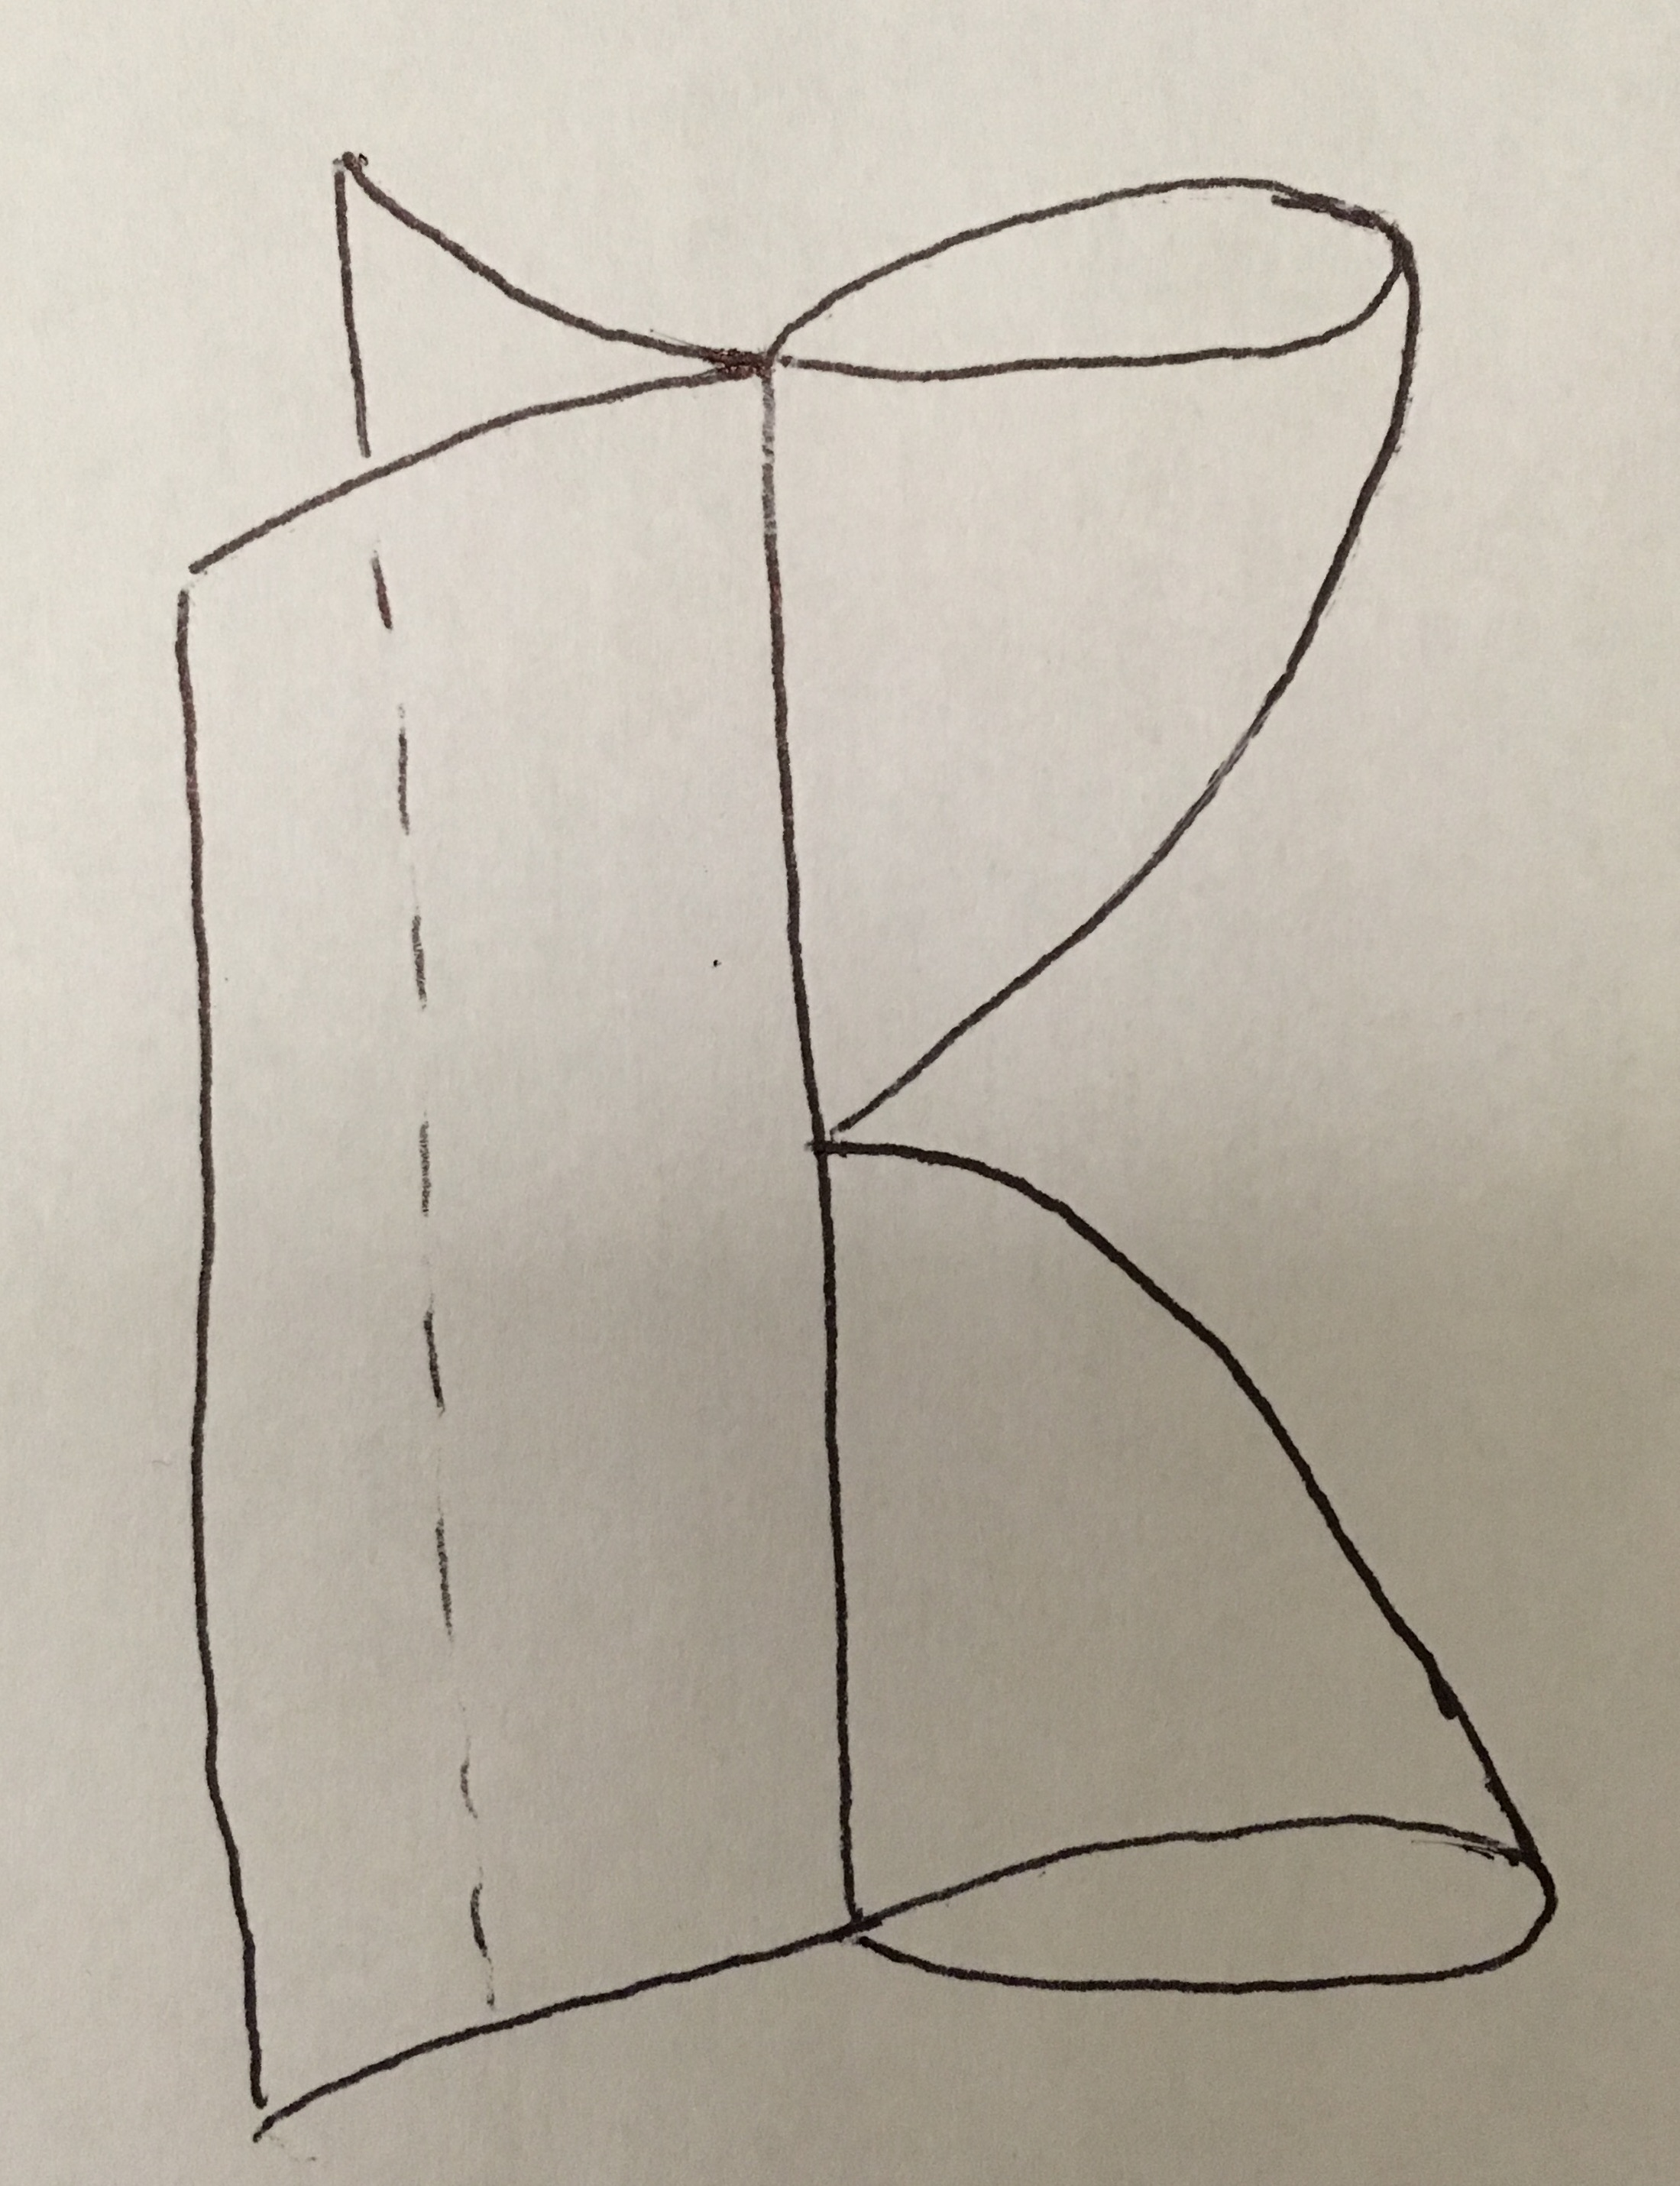
\includegraphics[width=40mm]{stratified.jpg}
\end{figure}
\end{definition}


\begin{prop}
The $i$-dimensional stratum of $X$ is an $i$-manifold.
\end{prop}


\begin{exmp} $ $
\begin{enumerate}
\item Complex algebraic varieties.
\item Complex analytic varieties.
\item Real algebraic varietes.
\item Real analytic varieties.
\item Real semi-algebraic varieties.
\item Subanalytic spaces.
\item Triangulated spaces.
\end{enumerate}
\end{exmp}

\begin{definition}
An $n$-dimensional stratified space is called a \textit{pseudomanifold} if $S_{n-1} = \emptyset$.
\end{definition}

\begin{exmp} $ $
\begin{enumerate}
\item Complex algebraic varieties.
\item Complex analytic varieties.
\item Triangulated spaces such that any $(n-1)$-simplex is the face of exactly two $n$-simplices. 
\end{enumerate}
\end{exmp}

\begin{theorem}
Every homology class can be represented by a pseudomanifold. 
\end{theorem}

\subsection{Lecture 18}

Let $X$ be an $n$-manifold. Let $R$ be a commutative ring. Note that $H_n(X, X \setminus x; R) \cong R$ for any $x\in X$.

\begin{definition}\label{RO}
  An \textit{$R$-orientation of $X$} is a locally compatible mapping $x\mapsto u_x$  such that $(u_x) = H_n(X, X \setminus x; R)$, i.e., $u_x$ is a unit.
\end{definition}

\begin{exmp}
Let $R= \Z/2$. Then there is exactly one choice of generator of $ H_n(X, X \setminus x; R)$. It's easy to show that the orientation cover of $X$ must be $X$ itself. This implies that any manifold has a $\Z/2$-orientation. It follows that $H_n(X; \Z/2) \cong \Z/2$ when $X$ is closed and connected. 
\end{exmp}

\section{Cohomology} 



Let $\left(C_{\ast}, \partial\right)$ be a chain complex of free abelian groups and $G$ be an abelian group. Let $$C_G^n \coloneqq  \Hom_{\Z}(C_n, G).$$ Define the \textit{coboundary map} $\delta : C_G^n \to C_G^{n+1}$ by $(\varphi : C_n \to G) \mapsto (c\mapsto \varphi(\partial{c}))$. Then $\delta^2 =0$. so that we get a \textit{cochain complex}
\[
\begin{tikzcd}
C_G^0 \arrow[r, "\delta"] & C_G^1 \arrow[r, "\delta"] & C_G^2 \arrow[r, "\delta"] & \cdots \arrow[r, "\delta"] & C_G^k \arrow[r, "\delta"] & C_G^{k+1} \arrow[r, "\delta"] & \cdots
\end{tikzcd}.
.\] Define the group of \textit{$k$-cocycles} as  $$Z_G^k = \ker(\delta: C_G^k \to C_G^{k+1})$$ and the group of \textit{$k$-coboundaries} as $$ B_G^k = \im(\delta : C_G^{k-1} \to C_G^k)  .$$ The \textit{$k$-th cohomology group of $C$ (with coefficients in $G$)} is $$H^k(C; G) = \faktor{ Z_G^k  }{B_G^k   }  .$$


\begin{note} 
 Let $\varphi \in Z_G^n$, so that $\delta{\varphi}=0$. Then $\varphi{\partial} =0$, which means that $B_n\subset \ker{\varphi}$. This induces a map $\tilde{\varphi} : H_n(C) \to G$.  We thus have an additive map $h: \varphi \mapsto \tilde{\varphi}$.

To see that $h$ is well-defined, suppose that $\varphi = \delta{\psi}$ for some $\psi : C_{n-1} \to G$. Then $\varphi = \psi{\partial}$, which implies that $\varphi$ vanishes on $Z_n$. Hence $\tilde{\varphi} =0$. This proves that $h: H^n(C; G) \to  \Hom_{\Z}(H_n(C); G)$ is well-defined.
\end{note}

\medskip

 Let $A$ and $B$ be abelian groups. There is a surjective map $f: F_0 \to A$ where $F_0$ is a free abelian group. Form a free resolution $F$ of $A$ $$0 \to F_1 \overset{i}{\longrightarrow} F_0 \overset{f}{\longrightarrow} A \to 0$$ where $F_1 \coloneqq  \ker{f}$. Consider the induced map $i^{\ast} : \Hom(F_0, B) \to \Hom(F_1, B)$ . Let $$\ext(A, B) \coloneqq  H^1(F; B) = \coker{i^{\ast}},$$ which is independent of our choice of $F$.

\begin{exmp} $ $
\begin{enumerate}
\item If $A$ is free, then $\ext(A, B) =0$. 
\item If $A = \Z/n$, then consider the free resolution $0 \to \Z \overset{n\cdot{-}}{\longrightarrow} \Z \to \Z \to 0$. This induces a map $$\Hom(\Z, B) \cong B \overset{n\cdot{-}}{\longrightarrow} \Hom(\Z, B) \cong B,$$ so that $\ext(\Z/n, B) \cong B/nB$.
\end{enumerate}
\end{exmp}

\begin{theorem}[Universal coefficient (for cohomology)]
There exists a non-canonical split short exact sequence $$\begin{tikzcd}
0 \arrow[r] & \ext(H_{n-1}(C), G) \arrow[r] & H^n(C; G) \arrow[r, "h"] & \Hom(H_n(C), G) \arrow[r] & 0
\end{tikzcd}     .$$
\end{theorem}

\begin{note} $ $
\begin{enumerate}
\item Let $X$ be a space and $C_{\ast}(X)$ our singular chain complex. Then $C^n(X; G) = \Hom(C_n(X), G)$. For any \textit{singular $n$-cochain} $\varphi$, we have that $$\delta{\varphi}(\sigma : \Delta^{n+1} \to X) = \sum_{k=0}^{n+1}({-1})^k\varphi(\sigma \restriction_{ [v_0, \ldots, \hat{v}_i, \ldots, v_{n+1}]}).$$ 
\item Any map $f: X \to Y$ of spaces induces a chain map $f_{\ast} : C_{\ast}(X) \to C_{\ast}(Y)$, which in turn induces a cochain map $f^{\ast} : C^{\ast}(Y; G) \to C^{\ast}(X; G)$ such that $\delta{f} = f{\delta}$.  We thus get a map on cohomology $f^{\ast} : H^n(Y; G) \to H^n(X;G)$, called the \textit{pullback of $f$}.
\item  {\textbf{(Reduced cohomology)}} Define the map $f : G \to C^n(X; G)$ by $g \mapsto c_g$ where $c_g$ denotes the constant map at $g$. Let $\widetilde{C}^{\ast}(X; G) \coloneqq  \coker{f}$, thereby defining $\widetilde{H}^{\ast}(X; G)$.

Then $\widetilde{H}^n(X; G) = H^n(X; G)$ when $n>0$. Note that $C^0(X; G)$ is precisely the group of functions $X \to G$. For any function $\varphi : X \to G$, we have that $\delta{\varphi}(\sigma) = \varphi(\sigma(1)) - \varphi(\sigma(0))$ for any $\sigma \in \sing_1(X)$. This shows that $\varphi$ is a cocycle if and only if it is constant on each path component of $X$. Thus, $$H^0(X; G) \cong \prod_{\pi_0(X)} G.$$ It follows that $\widetilde{H}^0(X; G)$ is precisely the group of all functions $X \to G$ constant on each path component of $X$ modulo the group of globally constant functions $X \to G$.
\item  {\textbf{(Relative cohomology)}} Let $(X, A)$ be a pair.  Note that $C_n(X,A)$ is isomorphic to the free abelian group with basis $\{\varphi : \Delta^n \to X \mid \im{\varphi} \subset X \setminus A\}$. Applying $\Hom({-}, G)$ to the short exact sequence $\eta: 0 \to C_n(A) \to C_n(X) \to C_n(X,A) \to 0$ yields the sequence $$ 0 \from C^n(A; G) \from C^n(X; G) \from C^n(X, A; G) \from 0  .$$ This is exact because $\eta$ splits. Thus, $$ C^n(X, A; G) \cong \{\varphi : \sing_n(X) \to G \mid \sigma : \Delta^n \to A \implies \varphi(\sigma) = 0\}.$$
\end{enumerate}
\end{note}

\begin{prop} $ $
\begin{enumerate}
\item  {\textbf{(Homotopy invariance)}} If $f \simeq g$ as maps $X \to Y$, then $f^{\ast} = g^{\ast}$ as maps $H^{\ast}(Y; G) \to H^{\ast}(X; G)$.
\item {\textbf{(Snake)}} Let $(X, A)$ be pair. There exists a \textit{long exact sequence in cohomology}
\[
\begin{tikzcd}
\cdots \arrow[r]         & {H^n(X, A)} \arrow[r] & H^n(X) \arrow[r] & H^n(A) \arrow[llld] \\
{H^{n+1}(X,A)} \arrow[r] & \cdots                &                  &                    
\end{tikzcd}
.\]
\item {\textbf{(Excision)}} Let $Z \subset A \subset X$ such that $\cl{Z} \subset \Int{A}$. Then $H^{\ast}(X, A; G) \cong H^{\ast}(X \setminus Z, A \setminus Z; G)$.
\item {\textbf{(MV sequence)}} Let $X = \Int{A} \cup \Int{B}$. Then there exists a LES
\[
\begin{tikzcd}
H^n(X) \arrow[r]     & H^n(A) \oplus H^n(B) \arrow[r] & H^n(A \cap B) \arrow[lld] \\
H^{n+1}(X) \arrow[r] & \cdots                         &                          
\end{tikzcd}
.\]
\end{enumerate}
\end{prop}

\begin{definition}
Let $X$ be a space and $R$ be a ring. Let $k, l \in \N$. Define the \textit{cup product} $C^k(X; R) \times C^l(X; R) \overset{\smile}{\longrightarrow} C^{k+l}(X; R)$ by $$\varphi \smile \psi(\sigma: \Delta^{k+l} \to X) = \varphi(\sigma \restriction_{\left[v_0, \ldots, v_k\right]}) \cdot_R \psi(\sigma \restriction_{v_k, \ldots, v_{k+l}}).$$
\end{definition}


The same definition works for relative singular cochain complexes. In general, if $f\in C^k(X, A; R)$ and $g \in C^l(X, B; R)$, then $f\smile g  \in  C^{k+l}(X, A \cup B; R) .$


\begin{prop} 
Let $\1 \in C^0(X; R)$ denote the constant map at $1_R$. Then $\1 \smile \varphi = \varphi \smile \1 = \varphi$.
\end{prop}

\begin{lemma}
$\delta(\varphi \smile \psi) = \delta{\varphi} \smile \psi + ({-1})^k \varphi \smile \delta{\psi}$.
\end{lemma}
\begin{proof}
We do the case where $\varphi, \psi \in C^1(X;R)$. If $\sigma \in \sing_3(X)$, then
\begin{align*}
 \left(\delta{\varphi} \smile \psi - \varphi \smile \delta{\psi}\right)(\sigma) & =   \delta{\varphi}([v_0, v_1, v_2])\psi([v_2, v_3]) -  \varphi([v_0, v_1])\delta{\psi}([v_1, v_2, v_3])
 \\ & =  \varphi([v_1, v_2])\psi([v_2, v_3]) - \varphi([v_0, v_2])\psi([v_2, v_3])  + \varphi([v_0, v_1])\psi([v_2, v_3]) 
 \\ & - \varphi([v_0, v_1])\psi([v_2, v_3]) + \varphi([v_0, v_1])\psi([v_1, v_3]) - \varphi([v_0, v_1])\psi([v_1, v_2])  
 \\ & = \delta(\varphi \smile \psi)(\sigma)
\end{align*}
\end{proof}

\begin{corollary}
The cup product descends to an operation $$ H^k(X, A;R) \times H^l(X,A;R) \overset{\smile}{\longrightarrow} H^{k+l}(X,A; R)     .$$
\end{corollary}

\subsection{Lecture 19}

\begin{exmp} $ $
\begin{enumerate}
\item Let $X= S_g$. By the universal coefficient theorem, we have that $$0 \to \ext(H_0(X), \Z) \to H^1(X; \Z) \to \Hom(H_1(X), \Z) \to 0.$$ Since $H_0(X) \cong \Z$ and $H_1(X) \cong \Z^{2g}$, it follows that $H^1(X; \Z) \cong \Z^{2g}$. 
\item Let $X= \RP^n$. 
\begin{center}
\resizebox{\columnwidth}{!}{
\begin{tabular}{ |c|c|c|c|c|c|c|c| } 
\hline
 $k$ &  $H_k$ & $\ext(H_{k-1}, \Z)$ & $\Hom(H_k, \Z)$  & $H^k(X; \Z)$  &  $\ext(H_{k-1}, \Z/2)$  & $\Hom(H_k, \Z/2)$  & $H^k(X; \Z/2)$   \\
\hline
 0 	  & $\Z$	 &  0	&  $\Z$	&  $\Z$	&  0	&  $\Z/2$	&  $\Z/2$	\\ 
  1 	  &  $\Z/2$	 &  0	&  0	& 0  	& 0	&  $\Z/2$	&  	 $\Z/2$ \\ 
 2 	  &  0	 &   $\Z/2$	& 0	&  $\Z/2$	&  $\Z/2$	& 0	&  	$\Z/2$ \\ 
  3 	  &  $\Z/2$	 &  0	&  0	&  0	&  	&  	&  	$\Z/2$ \\ 
 4 	  &  0	 &  $\Z/2$	&  0	&  $\Z/2$	&  	&  	& 	\\ 
 5 	  &  $\Z/2$	 &  0	&  0	&  	&  	&  	& 	\\ 
 6        &  0	 &  	&  	&  	&  	&  	& 	\\
\vdots &  \vdots	 &   	&   \vdots	&  \vdots 	&   \vdots	&  \vdots 	&  \vdots	\\
$n-2$ &    &  $\Z/2$	& 	 &  0	&  	&  	& 	\\
$n-1$ &  $\Z/2$   &  0	&  	&  $\Z/2$	&  	&  	&  	\\
 $n$   &  $\begin{cases} \Z & n \text{ odd} \\ 0 & n \text{ even} \end{cases}$  & $\begin{cases} \Z/2 & n \text{ odd} \\ 0 & n \text{ even} \end{cases}$  	& $\Z, \ n$\text{ odd} 	&  $\Z, \ n$\text{ odd}	&  	&  	&  $\Z/2, \ n$\text{ odd} 	\\
\hline
\end{tabular}  }
\end{center}
\item Let $0\leq k \leq 2n$. Then $H_k(\CP^n) \cong \begin{cases} \Z & k \text{ even} \\ 0 & k \text{ odd}   \end{cases}.$
\begin{prop}
If $X$ has torsion-free homology, then $H^n(X; \Z) \cong \Hom(H_n(X; \Z), \Z)$ for every $n$.
\end{prop}
Therefore, $$H^k(\CP^n; \Z) \cong \begin{cases} \Z & k \text{ even} \\ 0 & k \text{ odd}  \end{cases}.$$
\end{enumerate}
\end{exmp}

\begin{theorem}
If $R$ is commutative and $\varphi, \psi \in H^{\ast}(X, A; R)$, then $$\varphi \smile \psi = ({-1})^{\lvert{\varphi}\rvert\lvert{\psi}\rvert} \psi \smile \varphi$$ where $\lvert{\cdot}\rvert$ denotes the degree of a cocycle. That is, $\smile$ is \textit{graded commutative}.
\end{theorem}

\begin{remark}
At the same time, $\smile$ is \emph{not} graded commutative at the chain level. By contrast, the wedge product $\wedge$ of differential forms is graded commutative at the chain level. 
\end{remark}

\begin{exmp}
Let $X = S_g$. One can show that $H_1(X)$ has $(a_1, \ldots, a_g, b_1, \ldots, b_g)$ as a basis. Since $H^1(X;\Z) \cong \Hom(H_1(X), \Z)$ by the universal coefficient theorem, there exists a dual basis $\left(\alpha_1, \ldots, \alpha_g, \beta_1, \ldots, \beta_g\right)$ for $H^1(X; \Z)$. 
For each $1\leq i\leq g$, we want to represent each $\alpha_i$ by a cocycle $\varphi_i$ and each $\beta_i$ by a cocycle $\psi_i$. To this end, let $$\varphi_i(\sigma : \Delta^1 \to X) = \begin{cases} 1 & \sigma \cap \alpha_i \ne \emptyset \\ 0 & \sigma \cap \alpha_i = \emptyset     \end{cases}.$$ Define $\psi_i$ similarly. Assume that $g=2$. It is straightforward to verify that both $\delta{\varphi_i}$ and $\delta{\psi_i}$ vanish on each $2$-simplex inside $S_2$.
\begin{figure}[H]
\centering
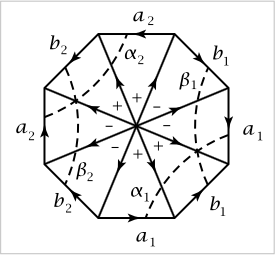
\includegraphics[width=40mm]{cup-prod-Sg.png}
\caption{copied from Hatcher (207) \label{overflow}}
\end{figure}
It is also straightforward to verify that $\varphi_1 \smile \psi_1$ vanishes on each $2$-simplex inside $S_2$ except the lower one marked by $b_1$, on which it equals $1$.
It follows that $\varphi_1 \smile \psi_1(c) =1$ where $c$ denotes the linear combination of the $2$-chains comprising $S_2$ with the indicated coefficients $\pm 1$. This shows that $[c]$ generates $H_2(X) \cong \Z$ and that $\varphi_1\smile \psi_1$ represents the dual generator $\gamma$ of $H^2(X; \Z) \cong \Z$. Hence $\alpha_1 \smile \beta_1 = [\gamma]$. In general, we can compute the relations
\begin{align*}
  \alpha_i \smile \beta_j & = 
  \begin{rcases}
    \begin{dcases}
   \gamma & i =j \\ 0 & i \ne j  
      \end{dcases}
  \end{rcases}
  \\ &  =  {-}(\beta_i \smile \alpha_j)
 \\  \alpha_i \smile \alpha_j & =0
 \\  \beta_i \smile \beta_j & =0
. \end{align*} These completely determine $H^1(X; \Z) \times H^1(X; \Z) \overset{\smile}{\longrightarrow} H^2(X; \Z)$ because $\smile$ is distributive.
\end{exmp}

\begin{definition}
Let $X$ and $Y$ be spaces. The \textit{external product} is the $R$-bilinear map $H^k(X; R) \times H^l(Y; R) \overset{\times}{\longrightarrow} H^{k+l}(X\times Y; R)$ given by $$ a\times b \equiv p_1^{\ast}{a} \smile p_2^{\ast}{b}$$ where $p_i$ denotes the $i$-th projection map for each $i=1,2$. 
Likewise, we define $H^k(X, A; R) \times H^l(Y, B; R) \overset{\times}{\longrightarrow} H^{k+l}(X\times Y, X\times B \cup A \times Y; R)$.
\end{definition}

By the universal property of the tensor product, this indues a unique linear map  
\[
 \label{eqn:cross}
H^k(X; R) \otimes_R H^l(Y; R) \overset{\times}{\longrightarrow} H^{k+l}(X\times Y; R).\tag{$\ast$}
\]

\smallskip

Let's return, for the moment, to the cup product. We can view $H^{\ast}(X; R)$ as a \textit{graded ring} $\left(\bigoplus_{k\geq 0} H^k(X; R), +, \smile\right)$, which induces a ring structure on $H^k(X; R) \otimes_R H^l(Y; R)$, namely
\[
\left(a \otimes b\right)\cdot \left(c \otimes d\right) \equiv ({-1})^{\lvert{b}\rvert \lvert{c}\rvert}\left(a \smile c\right) \otimes \left(b\smile d\right).
\]

\begin{prop}
The external product is a graded ring homomorphism, i.e., it is a ring morphism that preserves degree.
\end{prop}



\begin{theorem}[K\"unneth (special case)]\label{kunneth}
Suppose that  $X$ and $Y$ are CW-complexes such that $H^n(Y; R)$ is a finitely generated free $R$-module for each $n$. Then \eqref{eqn:cross} is a ring isomorphism, i.e.,  $$\bigoplus_{p+q= n} H^p(X; R) \otimes_R H^q(Y; R) \cong H^n(X\times Y; R)$$ for each $n$. 
\end{theorem}

\begin{remark}
We could drop the assumption that $X$ and $Y$ are CW-complexes.
\end{remark}

\begin{definition}
A \textit{cohomology theory $h^{\ast}$} on CW-pairs is a sequence of contravariant functors from CW-pairs to graded abelian groups that satisfies the following properties.
\begin{enumerate}[label=(\arabic*)]
\item If $f \simeq g$ as maps $X\to Y$, then $f^{\ast} = g^{\ast}$ as maps $h^{\ast}(Y) \to h^{\ast}(X)$.
\item $h^{\ast}(X, A) \cong h^{\ast}(X/A, \pt)$.
\item For any CW-pair $(X, A)$, there exists a LES
\[
\begin{tikzcd}
\cdots \arrow[r] & h^n(X, A) \arrow[r] & h^n(X) \arrow[r] & h^n(A) \arrow[r] & h^{n+1}(X, A) \arrow[r] & \cdots
\end{tikzcd}.
\]
\item $h^{\ast}\left(\bigvee_{\alpha} X_{\alpha}\right) \cong \prod_{\alpha} h^{\ast}(X_{\alpha})$.
\end{enumerate}
\end{definition}

\begin{lemma}
Let $\mu : h^{\ast}_1 \to h^{\ast}_2$ be a natural transformation of cohomology theories on CW-pairs. If $\mu(\pt, \emptyset) : h_1^{\ast}(\pt, \emptyset) \to h_2^{\ast}(\pt, \emptyset)$ is an isomorphism, then $\mu$ is an isomorphism for any CW-pair.
\end{lemma}
\begin{proof}
Due to the five lemma, it's enough to prove that for any CW-complex $X$, $\mu_X : h_1^{\ast}(X) \to h_2^{\ast}(X)$. Assuming that $X$ is finite-dimensional, we do this by induction on the dimension of $X$. Since $X^0$ is a discrete set of points, our base case holds almost by assumption.  

\medskip

 Suppose, inductively, that $\mu_{X^{n-1}}$ is an isomorphism. Since $\mu$ is a natural transformation, we get a commutative diagram with exact rows
\[
\begin{tikzcd}
{h_1^k(X^n, X^{n-1})} \arrow[r] \arrow[d, "\mu"] & h_1^k(X^n) \arrow[r] \arrow[d, "\mu"] & h_1^k(X^{n-1}) \arrow[r] \arrow[d, "\mu(\cong)"] & {h_1^{k+1}(X^n, X^{n-1})} \arrow[r] \arrow[d, "\mu"] & \cdots \\
{h_2^k(X^n, X^{n-1})} \arrow[r]                  & h_2^k(X^n) \arrow[r]                  & h_2^k(X^{n-1}) \arrow[r]                         & {h_2^{k+1}(X^n, X^{n-1})} \arrow[r]                  & \cdots
\end{tikzcd}.
\] By the five lemma, we must need to show that $\mu : h_1^k(X^n, X^{n-1}) \to h_2^k(X^n, X^{n-1})$ is an isomorphism. We have another commutative diagram
\[
\begin{tikzcd}
{h_1^k(X^n, X^{n-1})} \arrow[d, "\cong" description] \arrow[r, "\mu"]       & {h_2^k(X^n, X^{n-1})} \arrow[d, "\cong" description]       \\
h_1^k(X^n/X^{n-1}) \arrow[d, "\cong" description] \arrow[r, "\mu"]          & h_2^k(X^n/X^{n-1}) \arrow[d, "\cong" description]          \\
h_1^k\left(\bigvee_{\alpha} S^n\right) \arrow[d, "\cong" description] \arrow[r, "\mu"] & h_2^k\left(\bigvee_{\alpha} S^n\right) \arrow[d, "\cong" description] \\
\prod_{\alpha}h_1^k(S^n) \arrow[r, "\mu"]                                   & \prod_{\alpha}h_2^k(S^n)                                  
\end{tikzcd}
.\] Thus, we want to show that bottommost $\mu$ is an isomorphism. Since $S^{n-1}$ is an $(n-1)$-dimensional CW-complex and $D^n \simeq \pt$, applying the five lemma together with our IH to the LES for $(D^n, S^{n-1})$ proves that $h_1^k(S^n) \cong h_2^k(S^n)$.

\medskip

 The case where $X$ is infinite-dimensional reduces to the case where it's finite-dimensional. We omit the details. 
\end{proof}

\begin{prop}
Let $Y$ be a CW-complex and $H^{\ast}(Y; R)$ be free over $R$. Consider the functors 
\begin{align*} h^{\ast}_1(X, A)&  \equiv H^{\ast}(X, A; R) \otimes_R H^{\ast}(Y; R) \\ h_2^{\ast}(X, A) & \equiv H^{\ast}(X \times Y, A \times Y; R)
 \end{align*} where $X$ is a CW-complex. If $A= \emptyset$, then the map $\mu : h_1^{\ast}(X) \to h_2^{\ast}(X)$ given by $a \otimes b \mapsto a \times b$ defines a natural transformation $h_1^{\ast}({-}) \to h_2^{\ast}({-})$. 
\end{prop}

\begin{proof}[Proof of \cref{kunneth}]
It suffices to show that $\mu : h_1^{\ast}(X) \to h_2^{\ast}(X)$ is an isomorphism when $X = \pt$. But, in this case, $\mu$ is precisely the map $R\otimes_R H^n(Y; R) \to H^n(Y; R)$ given by $\ r \otimes y \mapsto ry$, which is a well-known isomorphism.  
\end{proof}

\begin{exmp}
 $H^{\ast}(S^n) \otimes  H^{\ast}(S^m) \cong H^{\ast}(S^n \times S^m)$.
 \end{exmp}

\subsection{Lecture 20}

We also have a relative version of \cref{kunneth}.

\begin{theorem}[K\"unneth (special case)]
Let $(X, A)$ and $(Y, B)$ be CW-pairs. If $H^k(Y, B; R)$ is a finitely generated free $R$-module for each $k$, then $$ H^{\ast}(X, A; R) \otimes_R H^{\ast}(X, B; R) \overset{\times}{\longrightarrow} H^{\ast}(X \times Y, A \times Y \cup X \times B; R)$$ is a ring isomorphism. 
\end{theorem}

\begin{definition}
Let $\left(X, x_0\right)$ and $\left(Y, y_0\right)$ be pointed spaces. The \textit{smash product $X \wedge Y$} is $$\left(X \times Y\right)/\left(X \times \{y_0\} \cup \{x_0\} \times Y\right).$$
\end{definition}

\begin{remark}
The smash product is a monoidal product in $\mathbf{Top}_{\ast}$.
\end{remark}

\begin{exmp} $ $
\begin{enumerate}
\item $S^n \wedge  S^m \cong S^{n+m}$.
\begin{proof}
 It suffices to show that if $\left(X, x_0\right)$ and $\left(Y, y_0\right)$ are compact manifolds, then $$X \wedge Y \cong \left(\left(X \setminus \{x_0\}\right) \times \left(Y \setminus \{y_0\}\right)\right)^{\ast}$$ where $({-})^{\ast}$ denotes the one-point compactification. Let $Z\coloneqq  \left(X \setminus \{x_0\}\right) \times \left(Y \setminus \{y_0\}\right)$. Note that $Z$ is noncompact but locally compact. 
 
 We see that $\psi \coloneqq  \pi \circ i : Z \to X \wedge Y$ is injective with $\im{\psi} = X \wedge Y \setminus \{(x_0, y_0)\}$. Let $U \subset Z$ be open. Then $U$ is open in $X \times Y$.  Since $\pi^{-1}(\pi(U)) = U$, it follows that $\pi(U)$ is open in $X \wedge Y$. Thus, $\psi$ is an open map, so that $\psi$ is a topological embedding. Since $X \wedge Y$ is compact, it follows that $\psi$ is a Hausdorff compactification. 
\end{proof}
\item $S^1 \wedge X \cong \left(X\times I\right)/\left(X\times \{0\}\cup X\times \{1\}\cup \{x_{0}\}\times I\right)$, called the \textit{reduced suspension $\Sigma{X}$ of $X$}.
\end{enumerate}
\end{exmp}

\begin{exmp} $ $
\begin{enumerate}
\item Let $\left(X, x_0\right)$ and $\left(Y, y_0\right)$ be pointed spaces with $H^{\ast}\left(Y, y_0\right)$ free and finitely generated over $\Z$. Then $H^{\ast}\left(X, x_0\right) \otimes H^{\ast}\left(Y, y_0\right) \cong H^{\ast}(X \times Y, X \times \{y_0\} \cup Y \times \{x_0\}) \cong H^{\ast}(X \wedge Y)    .$
\item  $\widetilde{H}(S^n) \times \widetilde{H}^m(S^m) \cong H^{n+m}(S^{n+m})$.
\end{enumerate}
\end{exmp}

\bigskip

\begin{note}
Any polynomial ring is graded since $R[x] = \bigoplus_{n \in \N} Rx^n$.
\end{note}

\begin{theorem}
Let $X = \CP^n$ (resp. $\RP^n$) and $R = \Z$ (resp. $\Z/2$), then $H^{\ast}(X; R) \cong \faktor{R[\tilde{x}]}{(\tilde{x}^{n+1})}$ where $\lvert{\tilde{x}}\rvert =2$ (resp. $1$).
\end{theorem}
\begin{proof}
See Theorem 3.19 (Hatcher) for a proof of the case where $X= \RP^n$. We will assume that $X = \CP^n$.

\medskip

 The inclusion $\CP^{n-1} \hookrightarrow \CP^n$ induces an isomorphism $H^k(\CP^{n-1}) \to H^k(\CP^n)$ when $k < 2n-1$. Thus, it suffices to show that if $\omega \in H^{2i}(\CP^n)$ is a generator and $\omega ' \in H^{2n -2i}(\CP^n)$ is a generator where $0\leq i \leq n$ is even, then $\omega \smile \omega '$ generates $H^{2n}(\CP^n)$. Set $j = n-i$. Then $\CP^j = \left\{[z_0, \ldots, z_n] \mid z_0 = z_1 = \cdots = z_{i-1}= 0\right\}$, and $$\CP^i \cap \CP^j = p\coloneqq  \left[0, \ldots, 0, \underbrace{1}_{i\text{-th spot}}, 0 \ldots, 0\right].$$ Note that $\CP^i \cap U \cong \C^i$ and $\CP^j \cap U \cong \C^j$ where $U = \{[x_0, \ldots, z_n] \mid z_i \ne 0\}$. Consider the commutative diagram
\[
\begin{tikzcd}
H^{2i}(\CP^n)\times H^{2j}(\CP^n) \arrow[r, "\smile"]                                                                                              & H^{2n}(\CP^n)                                                                 \\
{H^{2i}(\CP^n, \CP^n \setminus \C^j)\times H^{2j}(\CP^n, \CP^n \setminus \C^i)} \arrow[r, "\smile"] \arrow[u, "\varphi_1"] \arrow[d, "\varphi_2"'] & {H^{2n}(\CP^n, \CP^n \setminus \{p\})} \arrow[u, "\cong"'] \arrow[d, "\cong"] \\
{H^{2i}(\C^n, \C^n \setminus \C^j)\times H^{2j}(\C^n, \C^n \setminus \C^i)} \arrow[r, "\smile"]                                                    & {H^{2n}(\C^n, \C^n \setminus \{0\})}                                         
\end{tikzcd}
,\] where the top right isomorphism comes from the five lemma applied to the LES's for $(\CP^n, \CP^n \setminus \{p\})$ and $(\CP^n, \CP^{n-1})$ and the bottom right isomorphism comes from excision. 
\begin{claim}
Both $\varphi_1$ and $\varphi_2$ are isomorphisms. 
\end{claim}
\begin{proof}
We have a commutative diagram 
\[
\begin{tikzcd}
H^{2i}(\CP^n) \arrow[d, "\cong"'] & {H^{2i}(\CP^n, \CP^{i-1})} \arrow[l, "\cong"'] \arrow[d, "\cong"'] & {H^{2i}(\CP^n, \CP^n \setminus \CP^j)} \arrow[l, "\psi"'] \arrow[r, "\cong"] \arrow[d] & {H^{2i}(\C^n, \C^n \setminus \C^j)} \arrow[d] \\
H^{2i}(\CP^i)                     & {H^{2i}(\CP^i, \CP^{i-1})} \arrow[l, "\cong"]                      & {H^{2i}(\CP^i, \CP^i \setminus \{p\})} \arrow[l, "\gamma"] \arrow[r, "\cong"']                             & {H^{2i}(\C^i, \C^i \setminus \{0\})}           
\end{tikzcd}
,\] where \hl{the isomorphisms of the leftmost square come from cellular cohomology} and those from the rightmost square come from excision. It suffices to show that each map in this diagram is an isomorphism. Note that $\gamma$ is an isomorphism because $\CP^i \setminus \{p\}$ deformation retracts onto $\CP^{i-1}$. Hence it suffices to observe that $\psi$ is an isomorphism because $\CP^n \setminus \CP^{j}$ deformation retracts onto $\CP^{i-1}$. Indeed, $$\CP^n \setminus \CP^{j}= \left\{[z_0, \ldots, z_n] \mid \exists s \in \{0,1, \ldots, i-1\} \text{ such that } z_s \ne 0\right\},$$ so that the maps given by $f_t([z_0, \ldots, z_n])  = [z_0, \ldots, z_{i-1}, tz_i, \ldots, tz_n]$ ($1 \overset{t}{\rightarrow} 0$) define a suitable deformation retraction. 
\end{proof}
The map $H^{2i}(\C^n, \C^n \setminus \C^j)\times H^{2j}(\C^n, \C^n \setminus \C^i) \overset{\smile}{\longrightarrow} H^{2n}(\C^n, \C^n \setminus \{0\})$ is equivalent to the map $$H^{2i}(I^{2i}, \partial{I^{2i}})\times H^{2j}(I^{2j}, \partial{I^{2j}}) \overset{\smile}{\longrightarrow} H^{2n}(I^{2n}, \partial{I^{2n}}),$$ which maps any pair of generators to a generator by the K\"unneth theorem. 
By commutativity, it follows that $ H^{2i}(\CP^n)\times H^{2j}(\CP^n) \overset{\smile}{\longrightarrow} H^{2n}(\CP^n) $ also maps any pair of generators to a generator.  
\end{proof}

\begin{corollary} $ $
\begin{enumerate}
\item If $\R^n$ has a division algebra structure over $\R$, then $n =2^l$ for some $l\in \Z_{\geq 0}$. 
\item If $\C^n$ has a division algebra structure over $\C$, then $n=1$.
\end{enumerate}
\end{corollary}
\begin{proof} $ $
\begin{enumerate}
\item Suppose that $\R^n$ is a division algebra over $\R$. Then its bilinear product induces a continuous map $h: \RP^{n-1} \times \RP^{n-1} \to \RP^{n-1}$ such that $h\restriction_{\RP^{n-1} \times \{y\}}$ and $h\restriction_{\{x\} \times \RP^{n-1}}$ are homeomorphisms for any $x,y \in \RP^{n-1}$. The induced homomorphism $$h^{\ast}: \faktor{\Z_2\left[\tilde{x}\right]}{\left(\tilde{x}^n\right)} \to  \faktor{\Z_2\left[\tilde{x}_1, \tilde{x}_2\right]}{\left(\tilde{x}_1^n, \tilde{x}_2^n\right)}$$ is determined by the assignment $\tilde{x} \mapsto k_1 \tilde{x}_1 + k_2 \tilde{x_2}$. Since $h$ restricts to a homeomorphism on each copy of $\RP^{n-1}$, it follows that $k_1 \tilde{x}_1$ and $k_2\tilde{x}_2$ are nonzero. Hence $k_1 = 1 = k_2$. But $$0 = \tilde{x}^n = \left(\tilde{x}_1 + \tilde{x}^2\right)^n = \sum_{k=1}^{n-1} {n \choose k} \tilde{x}_1^k \tilde{x}_2^{n-k} .$$ This implies that ${n \choose k}\equiv 0 \mod 2$ for each $1\leq k \leq n-1$. 
\begin{exercise}
Use elementary number theory to prove this happens only if $n$ equals a power of $2$.
\end{exercise}
\item By a similar argument, we deduce that ${n \choose k} =  0$ for each $1\leq k \leq n-1$. This implies that $n=1$.
\end{enumerate}
\end{proof}

\begin{definition} Let $X$ be any space.
\begin{enumerate}
\item  We say that $X$ \textit{has category $n$} (written as $\cat(X) = n$) if $X$ can be written as a union of $n$ contractible open subsets but not $n-1$. 
\item The \textit{cup length $\clength(X)$ of $X$} is $ \max\{ c \in \Z \mid \exists x_1, \ldots, x_c \in H^{\ast}(X, \Z)$ such that $\lvert{x_i}\rvert \geq 1$ and $x_i\cdots x_c \ne 0\}$  .
\end{enumerate}
\end{definition}

\begin{exmp}
We know that $\CP^n = \bigcup_{i=0}^n U_i$ where $U_i \coloneqq  \{[z_0, \ldots, z_n] \mid z_i \ne 0\} \cong \C^n$. Is it possible to write $\CP^n$ as a union of $n$ contractible subspaces?
\end{exmp}

\begin{theorem}
If $X$ is a space, then $\cat(X) -1 \geq \clength(X)$.
\end{theorem}
\begin{proof}
Let $c \coloneqq  \cat(X)$. Then $X = \bigcup_{i=1}^c$ with each $U_i$ open and contractible. By the LES in cohomology, we get $H^j(X) \cong H^j(X, U_i)$ for any $i$ and any $j\geq 1$. Suppose that $x_i \in H^{j_i}(X)$ for each $1\leq i \leq c$ where $\lvert{x_i}\rvert \geq 1$. Then $x_1 \cdots x_c \in H^{j_1 + \cdots + j_c}(X, \bigcup_{i=1}^c U_i) = H^{j_1 + \cdots + j_c}(X, X)= 0$. Thus, $x_1 \cdots x_c =0$. 
\end{proof}

\begin{corollary}
$\cat(\CP^n) \geq \clength(\CP^n) +1 = n+1$.
\end{corollary}

\begin{definition}
Let $k\geq l$. The $\textit{cap product}$ is the map $C_k(X; R) \times C^l(X; R) \overset{\frown}{\longrightarrow} C_{k-l}(X; R)$ defined by $$ \sigma \frown  \varphi =  \varphi(\sigma \restriction_{[v_0, \ldots, v_l]})\sigma\restriction_{[v_l, \ldots, v_k]}.$$
\end{definition}

\begin{lemma}
$\partial(\sigma \frown\varphi) = ({-1})^l(\partial{\sigma} \frown \varphi - \sigma \frown \delta{\varphi})$.
\end{lemma}
\begin{proof}
We compute
\begin{align*}
 \partial{\sigma} \frown \varphi & = \sum_{i=0}^k ({-1})^i \sigma \restriction_{[v_0, \ldots, \hat{v}_i, \ldots, v_k]} \frown \varphi
 \\ & = \sum_{i=0}^l ({-1})^i \varphi (\sigma \restriction_{[v_0, \ldots, \hat{v}_i, \ldots, v_{l+1}]})\sigma \restriction_{[v_{l+1}, \ldots, v_k]} 
 \\ & + \sum_{i=l+1}^k ({-1})^i \varphi( \sigma \restriction_{[v_0, \ldots, v_l]}) \sigma \restriction_{[v_l, \ldots, \hat{v}_i, \ldots, v_k]}
 \\ \sigma \frown \delta{\varphi} & = \delta{\varphi(\sigma \restriction_{[v_0, \ldots, v_{l+1}]})}\sigma \restriction_{[v_{l+1}, \ldots, v_k]}
 \\ & = \sum_{i=0}^{l+1} ({-1})^i \varphi (\sigma \restriction_{[v_0, \ldots, \hat{v}_i, \ldots, v_{l+1}]})\sigma \restriction_{[v_{l+1}, \ldots, v_k]}
 \\ \partial(\sigma \frown \varphi) & =  \partial(\varphi(\sigma \restriction_{[v_0, \ldots, v_l]})\sigma \restriction_{[v_l, \ldots, v_k]})
 \\ & = \sum_{i=l}^k ({-1})^{i-l}\varphi(\sigma \restriction_{[v_0, \ldots, v_l]})\sigma \restriction_{[v_l, \ldots, \hat{v}_i, \ldots, v_k]}.
\end{align*}
It's easy to check that $({-1})^l \partial(\sigma \frown \varphi) = \partial{\sigma} \frown \varphi - \sigma \frown \delta{\varphi}.$
\end{proof}

\begin{corollary}
The cap product induces a map $H_k(X; R) \times H^l(X; R)  \overset{\frown}{\longrightarrow} H_{k-l}(X; R)$.
\end{corollary}
\begin{proof}
If $\sigma$ is a cycle and $\varphi$ a cocycle, then clearly $\sigma \frown \varphi$ is a cycle. Also, if $\sigma = \partial{d}$ and $\delta{\varphi}=0$, then $\sigma \frown \varphi = \partial{d} \frown \varphi = \pm \partial(d \frown \varphi)$. Hence the cap product of a boundary and cocycle is a boundary. Similarly, the cap product of a cycle and coboundary is a boundary.
\end{proof}

\begin{theorem}[Poincar\'e duality (PD)]
Let $X$ be a closed $R$-oriented $n$-manifold. Then the map $H^l(X; R) \to H_{n-l}(X;R)$ given by $\varphi \mapsto [X] \frown \varphi$ is an isomorphism for every $l$. 
\end{theorem}


PD is a global consequence of one local condition (manifold-hood) and two global conditions (orientability and closedness). 


\subsection{Lecture 21}


We have the following relative forms of the cap product.
\begin{align*}
H_k(X, A \cup B) \times H^l(X, A) & \overset{\frown}{\longrightarrow} H_{k-l}(X, B)
 \\ H_k(X, A) \times H^l(X) & \overset{\frown}{\longrightarrow} H_{k-l}(X, A)
 \\  H_k(X, A) \times H^l(X, A) & \overset{\frown}{\longrightarrow} H_{k-l}(X)
\end{align*}


\begin{prop}[Projection formula]
Let $f: X \to Y$ be a map of spaces. Let $[\sigma] \in H_k(X)$ and $[\varphi] \in H^l(Y)$. Then $$f_{\ast}([\sigma]) \frown [\varphi] = f_{\ast}([\sigma] \frown f^{\ast}([\varphi]))    $$ in $H_{k-l}(Y)$.
\end{prop}

\smallskip

Let $X$ be a locally compact CW-complex. Let $$C_c^i \coloneqq \left\{\varphi \in C^i(X; R) \mid \exists K_{\varphi}\subset X \text{ compact such that }\varphi(c) = 0 \text{ for any }c\in C_i(X \setminus K_{\varphi})\right\}.$$ This induces the \textit{cohomology group with compact support} $H^i_c(X; R)$.


\begin{note}
The groups $C^i_c(X;R)$ consisting of cochains $\varphi$ that are nonzero only on  $i$-simplices contained in some compact set $K_{\varphi}$ do not form a subcomplex of the singular cochain complex. Indeed, if $\varphi \in C^0(\R)$ has $\varphi(x_0) =1$ and $\varphi(x) =0$ for any $x\ne x_0$, then $\delta{\varphi}(\sigma : \underbrace{y \leadsto x_0}_{y\ne x_0}) = \varphi(\sigma(1)) - \varphi(\sigma(0)) \ne 0$.
\end{note}


Let  $X$ be a simplicial complex and let $C^i_c(X;G)$ denote the subgroup of compactly supported $i$-cochains. View $\R$ as a simplicial complex with vertices at the integer points. If $\varphi \in C^0_c$ satisfies $\delta{\varphi} =0$, then $\varphi$ must be constant since $\delta{\varphi}([n, n+1]) = \varphi(n+1) - \varphi(n)$ for every $n\in \Z$. In this case, $\varphi$ must be identically zero since it is compactly supported. Thus, $H^0_c(\R, \Z) =0$.

Define $\epsilon : C_c^1(\R; \Z) \to \Z$ by $ \epsilon(\psi) = \sum_{n\in \Z}\psi([n , n+1])$, which makes sense since $\psi$ is compactly supported. We have that $$\epsilon(\delta{\varphi}) = \sum_{n\in \Z} \delta{\varphi}([n, n+1]) = \sum_{n\in \Z} \varphi(n+1) - \varphi(n) =0.$$ Thus, $\epsilon$ vanishes on any coboundary. Since \hl{$\epsilon \ne 0$}, it follows that there are $1$-cocycles that are not coboundaries, so that $H_c^1(\R; \Z) \ne 0$. 

\begin{exercise}
Show that the induced map $\epsilon: H_c^1(\R; \Z) \to \Z$ is injective, i.e., if $\epsilon(\psi) =0$, then $\psi= \delta{\varphi}$ for some $\varphi$.
\end{exercise}


\begin{definition} $ $
\begin{enumerate}
\item Let $i$ be a poset. We say that $I$ is a \textit{directed set} if for any $\alpha, \beta \in I$, there exists $\gamma \in I$ such that $\alpha, \beta \leq \gamma$. 

Let $G_{\alpha}$ be an abelian group for each $\alpha \in I$. Suppose that for any $\alpha \leq \beta$, there is some homomorphism $f_{\alpha{\beta}} : G_{\alpha} \to G_{\beta}$ such that 
\begin{enumerate}[label=(\roman*)]
\item $f_{\alpha{\alpha}} = \1_{G_{\alpha}}$ for any $\alpha \in I$ and 
\item $f_{\beta{\gamma}}\circ f_{\alpha{\beta}} = f_{\alpha{\gamma}}$ when $\alpha \leq \beta \leq \gamma$. 
\end{enumerate}
Then $\{G_{\alpha}, f_{\alpha{\beta}}\}$ is called a \textit{directed system} of groups. 
\item Suppose that $\{G_{\alpha},  f_{\alpha{\beta}}\}$ is a directed system of groups. The \textit{direct limit} group is $$\varinjlim G_{\alpha} \equiv \faktor{\bigoplus_{\alpha \in I}G_{\alpha}}{N}$$ where $N$ is the subgroup generated by all elements of the form $a-f_{\alpha{\beta}}(a)$ with $a\in G_{\alpha}$. 

Equivalently, $\varinjlim G_{\alpha}$ has as its underlying set $\faktor{\coprod_{\alpha \in I} G_{\alpha}}{\sim}$ where $x_{\alpha} \simeq x_{\beta}$ if there exists $\gamma \in I$ such that $\alpha, \beta \leq \gamma$ and $f_{\alpha}{\beta}(x_{\alpha}) = f_{\beta{\gamma}}(x_{\beta})$. We equip this with the group structure $$[x_{\alpha}] +[x_{\beta}] = \left[f_{\alpha{\gamma}}(x_{\alpha}) + f_{\beta{\gamma}}(x_{\beta})\right]$$ where $\alpha, \beta \leq \gamma$. (This is well-defined because $I$ is a poset by hypothesis.)
\end{enumerate}
\end{definition}

\begin{aside}
Let $\mathbf{Ab}^I$ denote the category of directed systems (viewed as functors $I \to \mathbf{Ab}$), so that a morphism in $\mathbf{Ab}^I$ is precisely a collection of homomorphisms $\{w_{\alpha}\}: \{G_{\alpha}, f_{\alpha{\beta}}\} \to \{H_{\alpha}, g_{\alpha{\beta}}\}$ such that the square 
\[ \begin{tikzcd}
G_{\alpha} \arrow[d, "w_{\alpha}"'] \arrow[r, "f_{\alpha{\beta}}"] & G_{\beta} \arrow[d, "w_{\beta}"] \\
H_{\alpha} \arrow[r, "g_{\alpha{\beta}}"']                         & H_{\beta}                       
\end{tikzcd}
\] commutes for any $\alpha \leq \beta$. Let $a_{\alpha} : G_{\alpha} \to \varinjlim G_{\alpha}$ and $b_{\alpha} : H_{\alpha} \to \varinjlim H_{\alpha}$ denote the canonical maps. Then, by the universal property of colimits, the maps $b_{\alpha} \circ w_{\alpha} : G_{\alpha} \to  \varinjlim H_{\alpha}$ induce a unique map $w:  \varinjlim G_{\alpha} \to  \varinjlim H_{\alpha}$ such that $w \circ a_{\alpha} = b_{\alpha} \circ w_{\alpha}$.
The functor $\varinjlim : \mathbf{Ab}^I \to \mathbf{Ab}$ sends any morphism $\{w_{\alpha}\}$ to $w$.
\end{aside}

\smallskip

We have that $C_c^i(X; R) = \bigcup_{K \subset X} C^i(X, X \setminus K; R)$ with  $K$ compact in $X$. Note that the set $K_X$ of compact sets in $X$ is a directed set both under inclusion $\subset$ (for a directed system of homology groups) and under reverse inclusion $\supset$ (for a directed system of cohomology groups). 


\begin{prop}\label{prop25} $ $
\begin{enumerate} 
\item Let $I$ be a directed set. Let $X= \bigcup_{\alpha \in I}X_{\alpha}$ such that any compact set in $X$ is contained in some $X_{\alpha}$. Then $\varinjlim H_i(X_{\alpha}; G) \cong H_i(X; G)$ for each $i$.
\item $\varinjlim_{K_X} H^i(X, X \setminus X_{\alpha}; R) \cong H^i_c(X; R)$.
\end{enumerate}
\end{prop}

\smallskip

\begin{note}[De Rham homology]
Let $X$ be a smooth $n$-manifold and consider its de Rham cochain complex $\left(\Omega^i(X), d\right)$. The \textit{de Rham homology $H_i(X)$} arises from the chain complex given by $$\Omega_i(X) \equiv \Omega^i(X)^{\vee} = \R\left[\{f : \Omega^i(X) \to \R \mid f \text{ continuous}\}\right]$$ and $\partial{\xi} \equiv \xi{d}$. Note that $ \Omega^i(X)^{\vee}$ is compactly supported. 

Suppose that $X$ is closed and oriented. The linear functional $\Omega^n(X) \to \R$ given by $\omega  \mapsto \int_X \omega$ is called an \textit{$n$-current}. Let $S \subset X$ be a closed $k$-submanifold. Then $ \eta \mapsto \int_S d{\eta \restriction_S} = \int_{\partial{S}} \eta \restriction_S =0$ defines a $(k-1)$-current $\Omega^{k-1}(X) \to \R$. We can view an element of $\Omega_i(X)$ as a distribution-valued form.

Further, we can take the topological dual of $\left(\Omega_c^{\ast}(X), d\right)$, but it won't be compactly supported. This dual $\Omega_{\ast}^{\BM}(X)$ induces the so-called \textit{Borel-Moore homology of $X$}. Another version of PD states that if $X$ is an oriented $n$-manifold, then
\begin{align*}
H^k_{\dr, c}(X) & \cong H^{\dr}_{n-k}(X)
\\  H^k_{\dr}(X) & \cong  H^{\BM}_{n-k}(X) 
. \end{align*}
\end{note}

\medskip

Now, let $X$ be an $n$-manifold with orientation $x \mapsto \alpha_x$. Let $K \subset  L \subset X$ be a chain of compact subsets.  We have a commutative diagram
\[
\begin{tikzcd}
{H_n(X, X \setminus L; R)\times H^k(X, X \setminus L; R)} \arrow[r, "\frown"] \arrow[d, "i_{\ast}"', bend right=49]     & H_{n-k}(X; R) \\
{H_n(X, X \setminus K; R) \times H^k(X, X \setminus K ; R)} \arrow[ru, "\frown"'] \arrow[u, "i^{\ast}"', bend right=49] &              
\end{tikzcd}
.\] There exist unique $\mu_K \in H_n(X, X \setminus K)$ and $\mu_L \in H_n(X, X \setminus L)$ such that $\mu_K(x) = \alpha_x$ and $\mu_L(y) = \alpha_y$ for each $x\in K$ and each $y\in L$. By uniqueness, $i_{\ast}(\mu_L) = \mu_K$. By naturality of $\frown$, $$\mu_K \frown x = i_{\ast}(\mu_L) \frown x = \mu_L \frown i^{\ast}(x)$$ for any $x\in H^k(X, X \setminus K)$. Therefore, the direct limit (over $K_X$) of the maps $g_K : H^k(X, X \setminus K) \to H_{n-k}(X)$ given by $x \mapsto \mu_K \frown x$ induces the \textit{duality homomorphism} $$ D_X : H_c^k(X) \to H_{n-k}(X)  .$$


\subsection{Lecture 22}


Any  proper map of locally compact CW-complexes $f: X \to Y$ induces  a homomorphism $f^{\ast}: H_c^{\ast}(Y; R) \to H_c^{\ast}(X; R)$. It also induces a map $C_c(Y) \to C_c(X)$ where $C_c({-})$ where $C_c({\cdot})$ denotes the space of compactly supported  maps ${\cdot} \to \R$.

But we also have a \textit{wrong way functor} or an \textit{umkehr map} in that the inclusion $i: U \to V$ of open sets in $X$ induces a homomorphism $i_{!} : H_c^k(U; R) \to H_c^k(V; R)$. It also induces a map $C_c(U) \to C_c(V)$ since every CW-complex is paracompact and thus always admits subordinate partitions of unity.


\begin{note}
Let $U \subset V$ be an inclusion of open sets in $X$. By applying excision twice, we see that $\varinjlim_{K_U} H^k(X, X \setminus K) = \varinjlim_{K_V} H^k(X, X \setminus K).$
\end{note}

\begin{prop}\label{p3}
Let $X$ be an $R$-oriented $n$-manifold.  Let $U$ and $V$ be open in $X$ with $X = U \cup V$. Then there exists a commutative diagram up to sign
\[
\begin{tikzcd}
\cdots \arrow[r] & H^k_c\left(U \cap V\right) \arrow[r] \arrow[d, "D_{U \cap V}"] & H_c^k(U)\oplus H_c^k(V) \arrow[r] \arrow[d, "D_U \oplus {-}D_V"] & H_c^k(X) \arrow[r] \arrow[d, "D_X"] & H^{k+1}_c\left(U \cap V\right) \arrow[d, "D_{U \cap V}"] \arrow[r] & \cdots \\
\cdots \arrow[r] & H_{n-k}\left(U \cap V\right) \arrow[r]                         & H_{n-k}(U) \oplus H_{n-k}(V) \arrow[r]                           & H_{n-k}(X) \arrow[r]                & H_{n-k-1}\left(U \cap V\right) \arrow[r]                         & \cdots
\end{tikzcd}
.\]
\end{prop}

\begin{theorem}
Let $X$ be an $R$-oriented $n$-manifold.  Then $D_X : H_c^k(X) \to H_{n-k}(X)$ is an isomorphism for each $i$.
\end{theorem}
\begin{proof} $ $
\begin{steps}
\item If $X= U \cup V$ with $U$ and $V$ open and $D_U$, $D_V$, and $D_{U \cap V}$ are isomorphisms, then $D_X$ is an isomorphism.
\begin{proof}
Apply the five lemma to the diagram of \cref{p3}. 
\end{proof}
\item Suppose that $X$ equals the union of a sequence of open sets $U_1 \subset U_2 \subset \cdots$. If each $D_{U_i} : H^k_c(U_i) \to H_{n-k}(U_i)$ is an isomorphism, then so is $D_X$.
\begin{proof}
By excision, we have that $$H^k_c(U_i) \cong \varinjlim_{K_{U_i}}H^k(U_i, U_i \setminus K) \cong  \varinjlim_{K_{U_i}}H^j(X, X \setminus K) $$ for each $i$. From this, we see that there are natural maps $H^k_c(U_i) \to H^k_c(U_{i+1})$. Hence we can take $\varinjlim H^k_c(U_i) \cong H^k_c(X)$. Also, \cref{prop25}(1) implies that $\varinjlim H_{n-k}(U_i) \cong H_{n-k}(X)$, so that $D_X = \varinjlim D_{U_i}$. The direct limit  preserves any isomorphism  since it is a functor. Therefore, $D_X$ is an isomorphism.
\end{proof}
\begin{note}
Our proof of Step 2 works so long as the directed set is totally ordered.
\end{note}
\item If $X = \R^n$, then $D_X$ is an isomorphism. 
\begin{proof}
Note that $\R^n \cong \Int{\Delta^n}$. Therefore, $H^k_c(\R^n) \cong H^k(\Delta^n, \partial{\Delta^n})$. We can thus can view the map $D_X$ as the map $$\tau : H^k(\Delta^n, \partial{\Delta^n}) \to H_{n-k}(\Delta^n)$$ given by $x \mapsto [\Delta^n] \frown x$ where $\Delta^n$ denotes the identity map $\Delta^n \to \Delta^n$, which represents a generator of $H_n(\Delta^n, \partial{\Delta^n})$. If $k\ne n$, then $\tau$ is the automorphism of the trivial group. Suppose that $k=n$. Note that $H^n(\Delta^n, \partial{\Delta^n}) \cong \Hom(H_n(\Delta^n, \partial{\Delta^n}), R)$ by the universal coefficient theorem, where any generator of $H^n(\Delta^n, \partial{\Delta^n})$ is represented by a cocycle $\varphi$ such that $\varphi([\Delta^n])=1$. But then $$\tau(\varphi) = [\Delta^n] \frown \varphi = \varphi(\sigma \restriction_{[v_0, \ldots, v_n]})\id_{v_n} =\id_{v_n},$$ which represents a generator of $H_0(\Delta^n)$. Thus, $\tau$ is an isomorphism. 
\end{proof}
\item If $U$ is any open set in $\R^n$, then $D_U$ is an isomorphism.
\begin{proof}
Since $\R^n$ is second countable, we can write $U =\bigcup_{i\in \N} U_i$ where each $U_i \subset \R^n$ is an open ball. Let $V_i = \bigcup_{j \leq i} U_j$, so that $V_1 \subset V_2\subset \cdots$. 

We claim that each each $D_{V_i}$ is an isomorphism. To do this, we prove the slightly more general claim that if $Z_s$ is any finite union $\bigcup_{k=1}^s B_k$ of open balls in $\R^n$, then $D_{Z_s}$ is an isomorphism. The base case follows automatically from Step 3. The inductive step holds because both $Z_s$ and $Z_s\cap B_{s+1}$ equal the union of $s$ open balls, in which case Step 1 implies that $ D_{Z_s \cup B_{s+1}} = D_{Z_{s+1}}$ is an isomorphism.

Since $\bigcup_{i=1}^{\infty} V_i = U$ and each $D_{V_i}$ is an isomorphism, it follows from Step 2 that $D_U$ is an isomorphism.
\end{proof}
\item If $X$ is any finite or countable union of open sets each of which is homeomorphic to $\R^n$, then $D_X$ is an isomorphism.
\begin{proof}
Use a nearly identical proof to that of Step 4.
\end{proof}
\item If $X$ is any noncompact manifold, then $D_X$ is an isomorphism.
\begin{proof}
Let $\mathcal{U}$ denote the set of open $U\subset X$ such that $D_U$ is an isomorphism. Order $\mathcal{U}$ by inclusion. Any chain in $\mathcal{U}$  has an upper bound due to Step 2. By Zorn's lemma, it follows that $\mathcal{U}$  has  some maximal element $U_0$. If there exists $x\in X \setminus U_0$, then find a neighborhood $U_x$ of $x$ that is homeomorphic to $\R^n$. In this case, $D_{U_x}$ is an isomorphism due to Step 3 and $D_{U_x \cap U_0}$ is an isomorphism due to Step 4, so that $D_{U_x \cup U_0}$ is an isomorphism due to Step 1. But this is impossible since $U_0$ is maximal. Thus, $U_0 = X$.
\end{proof}
\end{steps}
\end{proof}

\begin{corollary}
If $X$ is a closed $R$-oriented manifold of odd dimension $n$, then $\chi(X) =0$.
\end{corollary}
\begin{proof}
We have that \begin{align*} \chi(X) &= \sum_i({-1})^i\rnk{H_i(X)} \\ & = \sum_i({-1})^i\rnk{H^{n-i}(X)} \\ &= \sum_i({-1})^i\rnk{H_{n-i}(X)} =0.\end{align*}
\end{proof}

\begin{exercise}
Let $X$ be a closed manifold. Use the universal coefficient theorem to show that the value $ \sum_i({-1})^i\rnk{H_i(X; \Z)}$ remains the same when $\Z$ is replaced by any $R$.  
\end{exercise}

\begin{corollary}
Since any manifold $X$ is $\Z/2$-oriented, $\chi(X) =0$ whenever $X$ is closed and $\dim{X}$ is odd. 
\end{corollary}

\begin{remark}
Take any finite-dimensional simplicial complex $X$ and embed $X$ into some $\R^N$. Take a tubular neighborhood $U$ of $X$ in $\R^N$. Then $U$ is a non-compact manifold such that $U \simeq X$. This suggests that the (co)homology of compact manifolds is much richer than that of non-compact ones. 
\end{remark}

\begin{exmp}
Let $X$ be a closed $R$-oriented $4$-manifold that is simply connected. By PD, we quickly get
$$H^k(X)  \cong \begin{cases} \Z & k = 0,4  \\ \pi_1(X)_{ab} =0 & k=3 \end{cases}   .$$ By the universal coefficient theorem, it follows that $H^1(X) =0$. Finally, the same theorem shows that $H_2(X) \cong H^2(X) \cong \Hom(H_2(X), \Z)$, which is a free abelian group since $H_2(X)$ is finitely generated. 
\end{exmp}

\begin{prop}
If $X$ and $Y$ are oriented $n$-manifolds, then $$ H^k(X \# Y) \cong \begin{cases}   H^k(X) \oplus H^k(Y) & 0 <k <n \\ \Z & k=0,n  \end{cases}    .$$
\end{prop}

\begin{definition}
Let $X$ be a closed $R$-orientable $n$-manifold. Consider the bilinear form $$B: H^k(X; R) \times H^{n-k}(X;R) \to R$$ given by $(f,g) \mapsto (f\smile g)[X]$. 
 We say that $B$ is \textit{nondegenerate} or \textit{nonsingular} if the induced maps $H^k(X; R) \to \Hom_R(H^{n-k}(X; R), R)$ and $H^{n-k}(X;R)  \to \Hom_R(H^k(X; R) , R)$ are both isomorphisms. 
\end{definition}

\begin{lemma}
If $\varphi \in C_k(X; R)$, $\psi \in C^l(X; R)$, and $\alpha \in C_{k+l}(X; R)$, then $\psi(\alpha \frown \varphi) = (\varphi \smile \psi)(\alpha)$.
\end{lemma}
\begin{proof}
We compute
\begin{align*}
\psi(\alpha \frown \varphi) & = \psi(\varphi(\sigma \restriction_{\left[v_0, \ldots, v_k\right]})\sigma \restriction_{[v_k, \ldots, v_{k+l}]})
\\  & =  \varphi(\sigma \restriction_{\left[v_0, \ldots, v_k\right]})\psi(\sigma \restriction_{[v_k, \ldots, v_{k+l}]}) =  (\varphi \smile \psi)(\alpha)
.\end{align*}
\end{proof}

\begin{theorem}
Our bilinear form $B$ is nondegenerate modulo torsion.
\end{theorem}
\begin{proof}
Consider the composite $$H^{n-k}(X ; R) \stackrel{h}{\longrightarrow} \operatorname{Hom}_{R}\left(H_{n-k}(X ; R), R\right) \stackrel{D^{*}}{\longrightarrow} \operatorname{Hom}_{R}\left(H^{k}(X ; R), R\right).$$ The map $h$ is obtained from the universal coefficient theorem and is an isomorphism modulo torsion. Moreover, $D^{\ast}{h}$ maps each $f \in H^{n-k}(X;R)$ to the homomorphism given by $g \mapsto f([X] \frown g) = (f\smile g)[X]$. Since $D$ is an isomorphism, it follows that $B$ is nondegenerate in its second factor. It is also nondegenerate in its first factor because of the commutativity of the cup product. 
\end{proof}


\begin{remark}
For any $4k$-manifold $X$, both $\rnk{H^{2k}}$ and the signature of $B : H^{2k} \times H^{2k} \to H^{4k}$ are \hl{topological} invariants over $\R$ where the \textit{signature of $B$} is $$\#\left(\text{positive eigenvalues of }B\right) - \#\left(\text{negative eigenvalues of }B\right).$$ The former, however, is the only such invariant over $\C$.
\end{remark}

\begin{theorem}[Friedman]
Any oriented closed simply connected $4k$-manifold is classified up to homeomorphism by the signature of $B$ (along with, sometimes, a $\Z/2$-valued invariant).
\end{theorem}

\subsection{Lecture 23}

\begin{definition}
Let $\H^n\coloneqq  \left\{(x^1, \ldots, x^n) \in \R^n : x_n \geq 0\right\}.$ An \textit{$n$-dimensional manifold with boundary} $M$ is a Hausdorff space such that for any $p \in M$, there exist a neighborhood $U$ of $p$ and a homeomorphism $\varphi : U \to \H^n$.  Any point $p\in M$ is called a \textit{boundary point} if it belongs to $\varphi^{-1}( \{x_n = 0\})$.
\end{definition}

\begin{prop} 
For any compact manifold with boundary $M$, there exists a \textit{collar neighborhood} of $\partial{M}$, i.e., an open $U\supset \partial{M}$ such that $U \cong \partial{M} \times [0,1)$.
\end{prop}

\begin{definition}
A manifold with boundary is \textit{$R$-oriented} if $M \setminus \partial{M} = \Int{M}$ is $R$-oriented.
\end{definition}

\begin{prop} 
Let $M$ be a compact $n$-manifold with boundary. Find $ \partial{M} \times [0,1)$ a collar neighborhood of $\partial{M}$. Then $$  H_n(M, \partial{M}; R) \cong H_n(M \setminus \partial{M}, \partial{M} \times (0, \epsilon))  .$$
\end{prop}

\begin{corollary}
If $M$ is $R$-oriented, then we obtain a relative fundamental class $[M] \in H_n(M, \partial{M}; R)$, which restricts to a given orientation at every point in $M \setminus \partial{M}$.
\end{corollary}

\begin{theorem}[Lefschetz duality]
Let $M^n$ be an $R$-oriented compact manifold with boundary. Then the map $D_M: H^k(M, \partial{M}; R) \to H_{n-k}(M; R)$ given by $D{\varphi} = [M] \frown \varphi$ is an isomorphism. 
\end{theorem}
\begin{proof}
We will suppress our notation for the coefficient ring $R$. Let $C$ denote the directed set of compact sets $K$ contained in a complement of collar neighbohood of $\partial{M}$. Observe that
\begin{align*}
H^k_c(\Int{M}) & \cong \varinjlim_{K_{\Int{M}}} H^k(\Int{M}, \Int{M} \setminus K)
\\ & \cong \varinjlim_{C} H^k(M, M \setminus K) \cong \varinjlim_{\epsilon{\text{-collars }}U} H^k(M, U)
\\ & \cong H^k(M, \partial{M}). 
\end{align*}
By PD, it follows that $$H^k(M, \partial{M}) \cong H^k_c(\Int{M}) \cong H_{n-k}(\Int{M}) \cong H_{n-k}(M)  .$$
\end{proof}


\begin{definition} $ $
\begin{enumerate}
\item A \textit{double (cochain) complex} is a commutative diagram 
\[
\begin{tikzcd}
\vdots                                       & \vdots                                       & \vdots                                       &        \\
{A^{0,2}} \arrow[u, "d"] \arrow[r, "\delta"] & {A^{1,2}} \arrow[u, "d"] \arrow[r, "\delta"] & {A^{2,2}} \arrow[u, "d"] \arrow[r, "\delta"] & \cdots \\
{A^{0,1}} \arrow[u, "d"] \arrow[r, "\delta"] & {A^{1,1}} \arrow[u, "d"] \arrow[r, "\delta"] & {A^{2,1}} \arrow[u, "d"] \arrow[r, "\delta"] & \cdots \\
{A^{0,0}} \arrow[u, "d"] \arrow[r, "\delta"] & {A^{1,0}} \arrow[u, "d"] \arrow[r, "\delta"] & {A^{2,0}} \arrow[u, "d"] \arrow[r, "\delta"] & \cdots
\end{tikzcd}
\] in $\mathbf{Ab}$ such that $d^2 = 0 = \delta^2$ and $d{\delta} + \delta{d} =0$.
\item If $\left(A^{\bullet, \bullet}, d^{\bullet}, \delta^{\bullet}\right)$ denotes a double complex, then the \textit{total complex $\tot(A)$ of $A$} is the single complex with $\tot(A)^n \equiv \bigoplus_{p+q = n} A^{p,q}$ and $d_{\tot(A)} \restriction_{A^{p,q}} \equiv  \delta + ({-1})^pd$.
\item If $\left(A^{\bullet, \bullet}, d^{\bullet}, \delta^{\bullet}\right)$ denotes a double complex, then define the \textit{cohomology of $A$} as $$H^{\ast}(A, d, \delta) = H^{\ast}(\tot(A), d_{\tot(A)}).$$
\end{enumerate}
\end{definition}

\begin{lemma}
Suppose that
\[
\begin{tikzcd}
\vdots                & \vdots                                   & \vdots                                       & \vdots                                       &        \\
0 \arrow[r] \arrow[u] & A^2 \arrow[r, "\epsilon"] \arrow[u, "d"] & {A^{0,2}} \arrow[r, "\delta"] \arrow[u, "d"] & {A^{1,2}} \arrow[r, "\delta"] \arrow[u, "d"] & \cdots \\
0 \arrow[r] \arrow[u] & A^1 \arrow[r, "\epsilon"] \arrow[u, "d"] & {A^{0,1}} \arrow[r, "\delta"] \arrow[u, "d"] & {A^{1,1}} \arrow[r, "\delta"] \arrow[u, "d"] & \cdots \\
0 \arrow[r] \arrow[u] & A^0 \arrow[r, "\epsilon"] \arrow[u, "d"] & {A^{0,0}} \arrow[r, "\delta"] \arrow[u, "d"] & {A^{1,0}} \arrow[r, "\delta"] \arrow[u, "d"] & \cdots
\end{tikzcd}
\] and 
\[
\begin{tikzcd}
\vdots                                        & \vdots                                        & \vdots                                        &        \\
{A^{0,1}} \arrow[r, "\delta"] \arrow[u, "d"]  & {A^{1,1}} \arrow[r, "\delta"] \arrow[u, "d"]  & A^{2.1} \arrow[u, "d"] \arrow[r, "\delta"]    & \cdots \\
{A^{0,0}} \arrow[r, "\delta"] \arrow[u, "d"]  & {A^{1,0}} \arrow[r, "\delta"] \arrow[u, "d"]  & {A^{2,0}} \arrow[u, "d"] \arrow[r, "\delta"]  & \cdots \\
A^0 \arrow[u, "\epsilon"] \arrow[r, "\delta"] & A^1 \arrow[u, "\epsilon"] \arrow[r, "\delta"] & A^2 \arrow[u, "\epsilon"] \arrow[r, "\delta"] & \cdots \\
0 \arrow[u] \arrow[r]                         & 0 \arrow[u] \arrow[r]                         & 0 \arrow[u] \arrow[r]               & \cdots
\end{tikzcd}
\]
are augmented double complexes with exact rows  and exact columns, respectively. Then there exists a cochain map $\left(A^{\bullet}, d\right) \to \left(\tot(A^{\bullet, \bullet}), d_{\tot}\right)$ that induces an isomorphism $H^{\ast}(A^{\bullet}, d) \to H^{\ast}(A^{\bullet, \bullet}, d, \delta).$
\end{lemma}
\begin{proof}
We just consider the case where the rows of $A^{\bullet, \bullet}$ are augmented. Note that $d_{\tot}{\epsilon} = (\delta + d){\epsilon} = d{\epsilon} = \epsilon{d}$. Hence $\epsilon^{\bullet}$ is a cochain map, thereby inducing a map $\epsilon^{\ast} : H^{\ast}(A^{\bullet}, d) \to H^{\ast}(A^{\bullet, \bullet}, d, \delta)$. We want to prove that $\epsilon^{\ast}$ is bijective. 

\medskip


Let $[c] \in H^{\ast}(A^{\bullet, \bullet}, d, \delta)$, so that $D(c) =0$. Write $c= (c_0, \ldots, c_n)$. Since each row is exact by hypothesis, there is some $s$ such that $\delta(s) = c_0$. We have that $c- d_{\tot}(s) = (0, c_1', \ldots, c'_n)$ for some $c_i'$. By repeating this procedure enough times, we get $[c] = [(0, \ldots, 0, v_n)]$ for some $v_n$. Note that $\delta(v_n) =0 = d(v_n)$. Hence there is some $z$ such that $\epsilon(z) = v_n$.   But $\epsilon(d(z)) = d(v_n) =0$, and $\epsilon$ is injective. Thus, $d(z) =0$. This proves that $$\epsilon([z]) = [(0, \ldots, 0, \epsilon(z))]  = [(0, \ldots, 0, v_n)] = [c],$$ so that $\epsilon^{\ast}$ is surjective.

\medskip

 Suppose that $\epsilon^{\ast}([v]) =0$, so that  $\epsilon(v) = d_{\tot}(p) = \delta \pm d(p)$ for some $p$. Note that $\delta(p) =0$. Thus, as before, we get $[p] = [(0, \ldots, 0, p_n)]$ for some $p_n$, so that $\epsilon(v) = D(0, \ldots, 0, p_n)$. This implies that $\delta(p_n) =0$. Since each row is exact, there is some $y$ such that $\epsilon(y) = p_n$. Then 
\begin{align*}
\epsilon(v) & = \delta(p_n) +d(p_n) 
\\ &= 0 + d(\epsilon(y))
\\ & =  \epsilon(d(y)).
\end{align*}
Since $\epsilon$ is injective, it follows that $v$ is a coboundary, i.e., $[v]=0$. Therefore, $\epsilon^{\ast}$ is injective. 
\end{proof}

\begin{definition}
Let $M$ be a smooth $n$-manifold and $\Lambda$ be a countable poset. An open cover $\left\{U_{\alpha}\right\}_{\alpha \in \Lambda}$ of $X$ is a \textit{good cover} if for any chain $\alpha_0\leq \cdots \leq \alpha_k$ in $\Lambda$, the space $$U_{\alpha_0\ldots \alpha_k}\coloneqq  U_{\alpha_0} \cap \cdots \cap U_{\alpha_k}$$ is either empty or diffeomorphic to $\R^n$.
\end{definition}


It is well known that every paracompact smooth $n$-manifold $M$ admits a Riemannian metric. Further, one can show that $M$ can be covered by finitely many geodesically convex open sets. Thus, $M$ has a finite good cover $\U \coloneqq  \{U_{\alpha_i}\}$.


\begin{definition} 
The \textit{\v{C}ech-de-Rham complex $\check{C}^{\bullet}(\U; \Omega^{\bullet})$} of $\U$ is the double complex
\[
\begin{tikzcd}
\vdots                                                                    & \vdots                                                                                           & \vdots                                                                                                            & \vdots                                                                                                                                   &        \\
\prod_{\alpha_0}\Omega^2(U_{\alpha_0}) \arrow[u, "d"] \arrow[r, "\delta"] & \prod_{\alpha_0{\alpha_1}}\Omega^2(U_{\alpha_0{\alpha_1}}) \arrow[u, "d"] \arrow[r, "\delta"] & \prod_{\alpha_0{\alpha_1{\alpha_2}}}\Omega^2(U_{\alpha_0{\alpha_1{\alpha_2}}}) \arrow[u, "d"] \arrow[r, "\delta"] & \prod_{\alpha_0{\alpha_1{\alpha_2{\alpha_3}}}}\Omega^2(U_{\alpha_0{\alpha_1{\alpha_2}{\alpha_3}}}) \arrow[r, "\delta"] \arrow[u, "d"] & \cdots \\
\prod_{\alpha_0}\Omega^1(U_{\alpha_0}) \arrow[u, "d"] \arrow[r, "\delta"] & \prod_{\alpha_0{\alpha_1}}\Omega^1(U_{\alpha_0{\alpha_1}}) \arrow[u, "d"] \arrow[r, "\delta"] & \prod_{\alpha_0{\alpha_1{\alpha_2}}}\Omega^1(U_{\alpha_0{\alpha_1{\alpha_2}}}) \arrow[u, "d"] \arrow[r, "\delta"] & \prod_{\alpha_0{\alpha_1{\alpha_2{\alpha_3}}}}\Omega^1(U_{\alpha_0{\alpha_1{\alpha_2}{\alpha_3}}}) \arrow[r, "\delta"] \arrow[u, "d"] & \cdots \\
\prod_{\alpha_0}\Omega^0(U_{\alpha_0}) \arrow[r, "\delta"] \arrow[u, "d"] & \prod_{\alpha_0{\alpha_1}}\Omega^0(U_{\alpha_0{\alpha_1}}) \arrow[r, "\delta"] \arrow[u, "d"] & \prod_{\alpha_0{\alpha_1{\alpha_2}}}\Omega^0(U_{\alpha_0{\alpha_1{\alpha_2}}}) \arrow[r, "\delta"] \arrow[u, "d"] & \prod_{\alpha_0{\alpha_1{\alpha_2{\alpha_3}}}}\Omega^0(U_{\alpha_0{\alpha_1{\alpha_2}{\alpha_3}}}) \arrow[r, "\delta"] \arrow[u, "d"] & \cdots
\end{tikzcd}.
\] where  $$\left(\delta{\omega}\right)_{\alpha_0 \ldots \alpha_{p+1}} \equiv \sum_{i=0}^{p+1}({-1})^i\omega_{\alpha_0\ldots \hat{\alpha}_i\ldots \alpha_{p+1}} \restriction_{U_{\alpha_0 \ldots \alpha_{p+1}}}  .$$
\begin{exmp}
Let $\omega \in \prod_{\alpha_0} \Omega^q (U_{\alpha_0})$. Then $\left(\delta{\omega}\right)_{\alpha_0{\alpha_1}} =\omega_{\alpha_1}\restriction_{U_{\alpha_0{\alpha_1}}} -\omega_{\alpha_0}\restriction_{U_{\alpha_0{\alpha_1}}}$. From this, we compute 
\begin{align*}
\left(\delta{\delta{\omega}}\right)_{\alpha_0{\alpha_1}{\alpha_2}} & = \left(\delta{\omega}\right)_{\alpha_1{\alpha_2}} \restriction_{U_{{\alpha_0}{\alpha_1}{\alpha_2}}} -  \left(\delta{\omega}\right)_{\alpha_0{\alpha_2}} \restriction_{U_{{\alpha_0}{\alpha_1}{\alpha_2}}} +  \left(\delta{\omega}\right)_{\alpha_0{\alpha_1}} \restriction_{U_{{\alpha_0}{\alpha_1}{\alpha_2}}}
\\ & = \omega_{\alpha_2} \restriction_{U_{{\alpha_0}{\alpha_1}{\alpha_2}}}  - \omega_{\alpha_1} \restriction_{U_{{\alpha_0}{\alpha_1}{\alpha_2}}} - \omega_{\alpha_2} \restriction_{U_{{\alpha_0}{\alpha_1}{\alpha_2}}} 
\\ & + \omega_{\alpha_0}  \restriction_{U_{{\alpha_0}{\alpha_1}{\alpha_2}}} + \omega_{\alpha_1} \restriction_{U_{{\alpha_0}{\alpha_1}{\alpha_2}}} - \omega_{\alpha_0} \restriction_{U_{{\alpha_0}{\alpha_1}{\alpha_2}}} 
\\ & = 0.
\end{align*}
\end{exmp}

\medskip

If $X$ is a space, then let $C_{lc}(X, \R)$ denote the additive group of locally constant functions $X \to \R$. Now, let  $\underline{\check{C}^{\bullet}(\U; \Omega^{\bullet})}$ denote the augmented \v{C}ech-de-Rham complex
\[
\begin{tikzcd}
\vdots                & \vdots                                           & \vdots                                                                    & \vdots                                                                                        & \vdots                                                                                                            &        \\
0 \arrow[r] \arrow[u] & \Omega^2(M) \arrow[r, "\epsilon"] \arrow[u, "d"] & \prod_{\alpha_0}\Omega^2(U_{\alpha_0}) \arrow[u, "d"] \arrow[r, "\delta"] & \prod_{\alpha_0{\alpha_1}}\Omega^2(U_{\alpha_0{\alpha_1}}) \arrow[u, "d"] \arrow[r, "\delta"] & \prod_{\alpha_0{\alpha_1{\alpha_2}}}\Omega^2(U_{\alpha_0{\alpha_1{\alpha_2}}}) \arrow[u, "d"] \arrow[r, "\delta"] & \cdots \\
0 \arrow[r] \arrow[u] & \Omega^1(M) \arrow[r, "\epsilon"] \arrow[u, "d"] & \prod_{\alpha_0}\Omega^1(U_{\alpha_0}) \arrow[u, "d"] \arrow[r, "\delta"] & \prod_{\alpha_0{\alpha_1}}\Omega^1(U_{\alpha_0{\alpha_1}}) \arrow[u, "d"] \arrow[r, "\delta"] & \prod_{\alpha_0{\alpha_1{\alpha_2}}}\Omega^1(U_{\alpha_0{\alpha_1{\alpha_2}}}) \arrow[u, "d"] \arrow[r, "\delta"] & \cdots \\
0 \arrow[r] \arrow[u] & \Omega^0(M) \arrow[r, "\epsilon"] \arrow[u, "d"] & \prod_{\alpha_0}\Omega^0(U_{\alpha_0}) \arrow[r, "\delta"] \arrow[u, "d"] & \prod_{\alpha_0{\alpha_1}}\Omega^0(U_{\alpha_0{\alpha_1}}) \arrow[r, "\delta"] \arrow[u, "d"] & \prod_{\alpha_0{\alpha_1{\alpha_2}}}\Omega^0(U_{\alpha_0{\alpha_1{\alpha_2}}}) \arrow[r, "\delta"] \arrow[u, "d"] & \cdots \\
                      &                                                  & {\prod_{\alpha_0}C_{lc}(U_{\alpha_0}, \R)} \arrow[r, "\delta"] \arrow[u]  & {\prod_{\alpha_0{\alpha_1}}C_{lc}(U_{\alpha_0{\alpha_1}}, \R)} \arrow[r, "\delta"] \arrow[u]  & {\prod_{\alpha_0{\alpha_1{\alpha_2}}}C_{lc}(U_{\alpha_0{\alpha_1{\alpha_2}}}, \R)} \arrow[r, "\delta"] \arrow[u]  & \cdots \\
                      &                                                  & 0 \arrow[u] \arrow[r]                                                     & 0 \arrow[u] \arrow[r]                                                                         & 0 \arrow[u] \arrow[r]                                                                                             & \cdots
\end{tikzcd}
\] where $\left(\epsilon{\omega}\right)_{\alpha_0} \equiv \omega \restriction_{U_{\alpha_0}}$. The cohomology of the bottom row of $\underline{\check{C}^{\bullet}(\U; \Omega^{\bullet})}$  is known as the \textit{\v{C}ech cohomology of $\U$ with coefficients in $\R$} and is denoted by $\check{H}^{\ast}(\U; \R)$.
\end{definition}

\begin{lemma}
The rows of $\underline{\check{C}^{\bullet}(\U; \Omega^{\bullet})}$ are exact.
\end{lemma}
\begin{proof}
It is clear that  $\delta{\epsilon}=0$. Since $\delta^2 = 0$, it just remains to check that $\ker{\delta} \subset \im{\delta}$ and $\ker{\delta} \subset \im{\epsilon}$.  Let $\omega \in \prod_{\alpha_0 \ldots \alpha_p} \Omega^q(U_{\alpha_0 \ldots \alpha_p})$ such that $\omega \in \ker{\delta}$. Then $\left(\delta{\omega}\right)_{\alpha \alpha_0 \ldots \alpha_p} =\omega_{\alpha_0 \ldots \alpha_p} + \sum_{i=0}^p ({-1})^{i+1} \omega_{\alpha \alpha_0\ldots \hat{\alpha}_i\ldots \alpha_p} = 0, $ so that $$\omega_{\alpha_0 \ldots \alpha_p}  =  \sum_{i=0}^p ({-1})^{i} \omega_{\alpha \alpha_0\ldots \hat{\alpha}_i\ldots \alpha_p}   .$$ 
Now, choose a partition of unity $\{\lambda_{\alpha}\}$ subordinate to $\U$. Define $s{\omega} \in \prod_{\alpha_0 \ldots \alpha_{p-1}} \Omega^q(U_{\alpha_0 \ldots \alpha_{p-1}})$ by $$\left(s{\omega}\right)_{\alpha_0 \ldots \alpha_{p-1}} = \sum_{\alpha} \lambda_{\alpha} \omega_{\alpha \alpha_0 \ldots \alpha_{p-1}}   .$$ We have that
\begin{align*}
\left(\delta{s\omega}\right)_{\alpha_0 \ldots \alpha_p}  & = \sum_{i=0}^p ({-1})^i \left(s\omega\right)_{\alpha_0 \ldots \hat{\alpha}_i \ldots \alpha_p}
\\ &  = \sum_{i=0}^p \sum_{\alpha} ({-1})^i \lambda_{\alpha} \omega_{\alpha \alpha_0 \ldots \hat{\alpha}_i \ldots \alpha_p}
\\ & = \sum_{\alpha} \sum_{i=0}^p ({-1})^i \lambda_{\alpha} \omega_{\alpha \alpha_0 \ldots \hat{\alpha}_i \ldots \alpha_p}
\\ & =  \sum_{\alpha} \lambda_{\alpha}\omega_{\alpha_0 \ldots \alpha_p} 
\\ & = \omega_{\alpha_0 \ldots \alpha_p}
. \end{align*}
This shows that $\delta{s{\omega}} =\omega$, so that $\omega \in \im{\delta}$, as desired. 
\medskip


 The fact that $\ker{\delta} \subset \im{\epsilon}$ is seen by gluing differential forms on $U_{\alpha}$ together to get a form on $M$.
\end{proof}

\begin{prop}\label{p4} Let $V$ be a smooth vector field and $\omega, \eta$ be differential forms. Let $\mathcal{L}$ denote the Lie derivative.
\begin{enumerate} 
\item  $i_V(\omega \wedge \eta) = i_V (\omega) + \eta  +({-1})^{\lvert{\omega}\rvert}\omega \wedge i_V{\eta}.$
\item {\textbf{(Cartan's magic formula)}}
$\mathcal{L}_V{\omega} = i_V{d(\omega)} + d(i_V{\omega}).$
\end{enumerate}
\end{prop}

\medskip

 Let $F: M \times I \to N$ be a smooth map where $N$ is a smooth manifold. Let $i_{{-}}$ denote interior multiplication. 
 For any $t\in I$, define $j_t: M \to M\times I$ by $j_t(p) = (p,t)$.
 For any $q\in \N$, define $\sigma  : \Omega^q(N) \to \Omega^{q-1}(M)$ by $$\left(\sigma{\omega}\right)_p = \left(x \mapsto \int_0^1 j_t^{\ast}i_{\frac{\partial}{\partial{t}}}(F^{\ast}{\omega})(x) dt\right)$$ where $x\in \bigwedge^{q-1}(T_p^{\ast}{M})$. 

\begin{lemma}[Poincar\'e]\label{Poin}
$(d\sigma + \sigma d)\omega = F_1^{\ast} \omega - F_0^{\ast}\omega$. That is, $\sigma$ is a cochain homotopy $F^{\ast}_0 \Rightarrow F^{\ast}_1$.
\end{lemma}
\begin{proof}
Using \cref{p4}, we compute
\begin{align*}
d\sigma \omega(x) + \sigma d \omega(x) & =  \int_0^1 dj_t^{\ast}i_{\frac{\partial}{\partial{t}}}(F^{\ast}{\omega})(x) dt + \int_0^1j_t^{\ast} i_{\frac{\partial}{\partial{t}}}(F^{\ast}{d\omega})(x) dt
\\ & =   \int_0^1 j_t^{\ast}di_{\frac{\partial}{\partial{t}}}(F^{\ast}{\omega})(x) dt + \int_0^1 j_t^{\ast}i_{\frac{\partial}{\partial{t}}}(dF^{\ast}{\omega})(x) dt
\\ & = \int_0^1 j_t^{\ast}\mathcal{L}_{\frac{\partial}{\partial{t}}}{F^{\ast}{\omega}}(x)dt
 . \end{align*} Note that the flow of $\left(0, \frac{\partial}{\partial{t}}\right)$ is given by $\theta_t(p,s) = (p, t+s)$. Hence $F \circ \underbrace{\theta_t \circ j_0}_{j_t} = F_t$. It follows that
\begin{align*}
j_t^{\ast}\mathcal{L}_{\frac{\partial}{\partial{t}}}{F^{\ast}{\omega}}
& = j_0^{\ast} \theta_t^{\ast}\mathcal{L}_{\frac{\partial}{\partial{t}}}{F^{\ast}{\omega}}
\\ & =  j_0^{\ast}\frac{d}{dt}\theta_t^{\ast}F^{\ast}\omega
\\ & = \frac{d}{dt}j_0^{\ast}\theta_t^{\ast}F^{\ast}\omega
\\ & = \frac{d}{dt}F_t^{\ast}{\omega}
. \end{align*}
 As a result, we can use Stokes' theorem to get
  \begin{align*}
d\sigma \omega(x) + \sigma d \omega(x) & =  \int_0^1 j_t^{\ast}\mathcal{L}_{\frac{\partial}{\partial{t}}}{F^{\ast}{\omega}}(x)dt
\\ & = \int_0^1 \frac{d}{dt}F_t^{\ast}{\omega}(x)dt
\\ & = \int_0^1 dF_t^{\ast}{\omega}(x)
\\ & = F^{\ast}_1{\omega}(x) - F^{\ast}_0{\omega}(x)
 . \end{align*}
\end{proof}

\begin{corollary}
If $U \cong \R^n$, then the sequence $$\R \to \Omega^0(U) \to \Omega^1(U) \to \Omega^2(U) \to \cdots$$ is exact. Therefore, the columns of $\underline{\check{C}^{\bullet}(\U; \Omega^{\bullet})}$ are also exact.
\end{corollary}
\begin{proof}
It is easy to check that our sequence is exact at $\Omega^0(U)$. We must show that it is exact at any $\Omega^i(U)$ with $i\geq 1$. There is some homotopy $F: U \times I  \to U$ such that $F_0 = c_x$ and $F_1 = \id_U$.  Let $\omega \in \Omega^i(U)$. We have that $(d \sigma + \sigma d) \omega = F_1^{\ast} \omega - F_0^{\ast} \omega = \omega -0 =\omega$. Hence $d \sigma + \sigma d = \1_{\Omega^i(U)}$.
\end{proof}

\begin{corollary}
 If $\U$ is a finite good cover of $M$, then $H^{\ast}_{\dr}(M) \cong  \check{H}^{\ast}(\U; \R)$.
\end{corollary}

\smallskip

Let $M$ be a smooth manifold and let $\left(\Omega^{\ast}(M), d\right)$ denote the cochain complex of differential forms. Then, by definition, $H_{\dr}^{\ast}(M) = H^{\ast}(\Omega^{\ast}(M), d)$. 

\begin{theorem}[De Rham]
 If $M$ is  paracompact, then $$H^{\ast}_{\dr}(M) \cong H^{\ast}(M; \R)$$ as graded rings.
\end{theorem}
\begin{proof}
Choose a finite good cover $\U$ of $M$. We have just proven that $H^{\ast}_{\dr}(M) \cong  \check{H}^{\ast}(\U; \R)$. By a similar argument, we can also show that $H^{\ast}(M; \R) \cong \check{H}^{\ast}(\U; \R)$.
\end{proof}

\section{Sheaves on spaces}

\subsection{Lecture 24}

Let $X$ be a space and $\Op(X)$ denote the category of open sets in $X$.

\begin{definition}
 A \textit{presheaf on $X$} is a functor $F: \Op(X)^{\op} \to \mathbf{Ab}$ such that $F(\emptyset) =0$. If $V\subset X$ is open, then any $s\in F(V)$ is called a \textit{section of $U$}. If $i : U \hookrightarrow V$, then $F(i): F(V) \to F(U)$ is called a \textit{restriction morphism} and is denoted by $r_{UV}$. 
\end{definition}

\begin{notation}
$r_{UV}(s)\coloneqq  s \restriction_U$.
\end{notation}

\smallskip

Let $\mathbf{PreSh}_X$ denote the category of presheaves on $X$.


\begin{note}[\v{C}ech cohomology]
We can build a cohomology theory of presheaves as follows. Let $X$ be a space with $\mathcal{U}$ an open cover. Let $F$ be a presheaf on $X$.  Let $\check{C}(\mathcal{U}, F)$ denote the chain complex
$$   \prod_{\alpha_0}F(U_{\alpha_0}) \overset{\delta}{\longrightarrow} \prod_{\alpha_0\alpha_1} F(U_{\alpha_0 \alpha_1}) \overset{\delta}{\longrightarrow} \prod_{\alpha_0\alpha_1\alpha_2}F(U_{\alpha_0\alpha_1\alpha_2}) \overset{\delta}{\longrightarrow} \cdots 
$$  where for any $f = \left(\underbrace{f_{\alpha_0\ldots \alpha_p}}_{\text{in }F(U_{\alpha_0\ldots \alpha_p})}\right)$, we have $$\left(\delta{f}\right)_{\alpha_0 \ldots \alpha_{p+1}} \equiv \sum_{i=0}^{p+1} ({-1})^i f_{\alpha_0 \ldots \hat{\alpha}_i \ldots \alpha_{p+1}} \restriction_{U_{\alpha_0\ldots \alpha_{p+1}}}.$$ Define the \textit{$p$-th \v{C}ech cohomology group} as $$\check{H}^p(X, F) = \varinjlim_{\mathcal{R}} \check{H}^p(\mathcal{U}, F)  $$ where $\mathcal{R}$ denotes the set of all open covers of $X$ ordered by refinement. 
\end{note}

\smallskip

\begin{definition}[Sheaf]
A presheaf $F$ on $X$ is a \textit{sheaf} if for any open $U \subset X$ and any open cover $\left\{U_{\alpha}\right\}$ of $U$, we have an exact sequence $$    0 \to F(U) \to \prod_{\alpha} F(U_{\alpha}) \overset{\tau}{\longrightarrow} \prod _{\alpha_0\alpha_1} F(U_{\alpha_0 \alpha_1})  $$ where $\left(\tau{f}\right)_{\alpha_0 \alpha_1} \equiv f_{\alpha_1}\restriction_{U_{\alpha_0\alpha_1}} - f_{\alpha_0} \restriction_{U_{\alpha_0\alpha_1}}$.
\end{definition}

Let $\mathbf{Sh}_{X}$ denote the category of sheaves on $X$, which is a full subcategory of $\mathbf{PreSh}_X$.

\begin{exmp} $ $
\begin{enumerate}
\item If $X$ is a manifold, then the assignment $U \mapsto \Omega^q(U)$ defines a sheaf. Indeed, let $g,f \in \Omega^q(U)$ such that $f \restriction_{U_{\alpha}} = f \restriction_{U_{\alpha}}$ for any $\alpha$. Then $g=f$. Moreover, if $f_{\alpha}\in \Omega^q(U_{\alpha})$ satisfies $f_{\alpha}\restriction_{U_{\alpha \beta}} = f_{\beta} \restriction_{U_{\alpha \beta}}$ for every $\beta$, then there is some $f \in \Omega^q(U)$ such that $f \restriction_{U_{\alpha}} = f_{\alpha}$.
\item Given an  abelian group $A$, the \textit{constant presheaf with value $A$} is given by $F(U) = A$. This is not a sheaf. Let $U$ and $V$ be any two spaces. Then $\{U, V\}$ is a cover for $U \coprod V$, but $$0 \to F(U \coprod V) \to F(U) \times F(V) \to F\left(U \cap V\right)$$ is not exact.
\item Given a set $A$ endowed with the discrete topology, the \textit{constant sheaf with value $A$}  is given by $$U \mapsto \{ f : U \to A \mid f \text{ locally constant}\} =   \{ f : U \to A \mid f \text{ continuous}\}.$$ This is denoted by  $\underline{A}$.
\item If $X$ is a holomorphic manifold, then we have a sheaf $\mathcal{O}({-})$ of holomorphic functions on open subsets of $X$.
\item The assignment sending each $U$ to the group $C(U)$ of functions $U \to \R$ is a sheaf.
\item  The assignment sending each $U$ to the group $C_b(U)$ of bounded continuous functions $U \to \R$ is a presheaf but not a sheaf. Indeed, for each $i\in \Z$, define $f_i : U_i \to \R$ by $f_i(x) = x$ where $U_i \coloneqq \left(i-1, i+1\right)\subset \R$. Each $f_i \in C_b(U_i)$, but you cannot glue the $f_i$ to a global bounded continuous function.  
\end{enumerate}
\end{exmp}

\begin{definition} 
Let $F$ be a presheaf on $X$ and $x\in X$. Define \textit{the stalk $F_x$ of $F$ at $x$} as $\varinjlim_{U \ni x}F(U)$.
\end{definition}

\begin{exmp} $ $
\begin{enumerate}
\item For any $x \in X$, $\underline{A}_x =A$.
\item The \textit{germs of continuous functions at $x$} are precisely the elements of $$C_x = \faktor{  \left\{(U, f) \mid x\in U, \ f \in C(U)\right\}    }{\sim}$$ where $(U, f) \sim(V, g)$ if $f =g$ on $U \cap V$.
\item Let $X = \R$. Let $C^{\infty}({-})$ denote the sheaf of smooth functions on $X$. Then we have an exact sequence $$ 0 \to \left(\text{flat functions}\right) \to C_0^{\infty} \to \R[\![x]\!] \to 0   .$$
\item Let $\mathcal{A}$ denote the sheaf of real analytic functions. Then $\mathcal{A}_0 \cong \R\{x\}$, the ring of real analytic functions.
\end{enumerate}
\end{exmp}

\begin{definition}
Let $F$ be a presheaf on $X$. Let $U \subset X$ be open and $s \in F(U)$. Define $\bar{s} : U \to  \coprod_{x\in X} F_x$ by $x \mapsto (x, (U, s))$. Define the \textit{\'etal\'e space of $F$} as $$\Et(F)   =  \left(\coprod_{x\in X} F_x, \tau \right), \ \quad \tau =\left\{S \subset \Et(F) \mid \bar{s}^{-1}(S) \text{ is open}, \ s \in F(U), \ U\subset X \right\}.    $$ 
\end{definition}

Equivalently, $\tau$ is generated by sets of the form $\Et(U, s) \coloneqq  \{(U, s_x) \mid x \in U\}$.

\begin{prop}
The natural projection $\pi : \Et(F) \to X$ is a local homeomorphism. 
\end{prop}

\smallskip

We have a functor $\mathbf{PreSh}_X \overset{+}{\longrightarrow} \mathbf{Sh}_{X}$ given by $F \mapsto F^{+}$ where $F^{+}$ is given by $$U \mapsto \{s : U \to \Et(F) \mid \pi s(x) = x \text{ and } s \text{ is continuous}\}  .$$ This is left adjoint to the forgetful functor $\mathbf{Sh}_{X} \to \mathbf{PreSh}_X$.


\subsection{Lecture 25}

\begin{lemma}
Let $F, G \in \ob{\mathbf{Sh}_{X}}$ and $f,g : F \to G$. 
\begin{enumerate}[label=(\alph*)]
\item If $f_x = g_x$ for every $x \in X$ where $g_x, f_x : F_x \to G_x$, then $f =g$.
\item $f_x : F_x \to G_x$ is injective for every $x$ if and only if $f_U : F(U) \to G(U)$ is injective for every open $U \subset X$.
\item $f_x : F_X \to G_x$ is an isomorphism if and only if $f$ is an isomorphism.
\end{enumerate}
\end{lemma}
\begin{proof} $ $
\begin{enumerate}[label=(\alph*)]
\item Consider the commutative square 
\[ \label{eqn:CS}
\begin{tikzcd}
F(U) \arrow[r, "\alpha"] \arrow[d] & \prod_{x\in U}F_x \arrow[d, "\prod_{x \in U}f_x = \prod_{x \in U} g_x "] \\
G(U) \arrow[r, "\beta"']           & \prod_{x \in U} G_x                                                     
\end{tikzcd}
.\tag{$\ast$}\]  
Note that $\alpha$ and $\beta$ are injective by sheaf-hood. Since $f_x = g_x$ for every $x\in U$, we can replace $f(U)$ by $G(U)$ and still make our square commute.
\item This follows from \eqref{eqn:CS}.
\item Part (b) shows that $f(U) : F(U) \to G(U)$ is injective. Hence we must show that it's surjective. Let $s \in G(U)$. For any $x \in U$, there exist $U_x \ni x$ and $s^x \in F(U_x)$ such that $f(s^x)_x = s_x$. Now use sheafiness to glue the $s^x$ together.
\end{enumerate}
\end{proof}

\begin{prop}
There exists a natural transformation  $\1 \overset{U}{\longrightarrow} +$ that is an isomorphism on stalks, i.e., $U_x : F_x \to F_x^{+}$ is an isomorphism for every $x$.
\end{prop}

\smallskip

Given any $f : F \to G$ with $F, G \in \ob{\mathbf{Sh}_{X}}$, let $\ker{f}(U) \equiv \ker(f(U) : F(U) \to G(U))$ for each open $U\subset X$. Then $\ker{f}$ is a sheaf. Let $\coker^{-}{f}(U) \equiv \coker(f(U) : F(U) \to G(U))$. This induces a presheaf $\coker^{-}{f}$. Finally, let $\coker{f} \equiv {\coker^{-}{f}}^{+}$.



\begin{prop}
$\mathbf{Sh}_{X}$ is an abelian category. 
\end{prop}

\begin{exercise}
Show that there are no projectives in $\mathbf{Sh}_{X}$.
\end{exercise}

Our next result is an application of Zorn's lemma.

\begin{prop}[Baer]
Let $I$ be a right $R$-module. Then $I$ is injective if and only if for any right ideal $J \unlhd R$, any map $\alpha : J \to I$ extends to a map $\tilde{\alpha} : R \to I$.
\end{prop}

\begin{corollary}
There are \textit{enough injectives} in $R^{\op}{-}\mathbf{Mod}$, i.e., any object can be embedded in an injective object. 
\end{corollary}

\begin{prop}
There are enough injectives in $\mathbf{Sh}_{X}$. 
\end{prop}
\begin{proof}
If $\{I_x\}_{x\in X}$ denotes a family of abelian groups , then define $\underline{I}(U) = \prod_{x\in U} I_x$ and $\Hom_{\mathbf{Sh}}(F, \underline{I}) = \prod_{x\in X} \Hom(F_x, I_x)$. As a result, if $I_x$ is injective (i.e., divisible), then $I$ will be injective. Given any sheaf $F$, choose $I_x$ injective such that $F_x \hookrightarrow I_x$. By doing this, we can form an injective object $I$ so that $0 \to F \to I$ is exact. 
\end{proof}

\begin{definition}
Given any diagram of sheaves $$  0 \to A \overset{i}{\longrightarrow} B \overset{j}{\longrightarrow} C \to 0  ,$$ we say that this is \textit{exact} if $0 \to A_x  \overset{i_x}{\longrightarrow}  B_x  \overset{j_x}{\longrightarrow}  C_x \to 0$ is exact for each $x\in X$. 
\end{definition}

\begin{prop}
If $0 \to A \to B \to C \to 0$ is exact in $\mathbf{Sh}_{X}$, then $0 \to A(X) \to B(X) \to C(X)$ is exact in $\mathbf{Ab}$.
\end{prop}

\begin{exmp}
 Let $X = \C^{\times}$. Then $$ 0 \to \underline{\Z} \overset{i}{\longrightarrow} \mathcal{O}_X \overset{g}{\longrightarrow} \mathcal{O}_X^X \to 0$$ is exact where $\mathcal{O}_X^X(U) \equiv \{ \varphi : U \to \C$ holomorphic $\mid \varphi(x) \ne 0$ for any $x\in U\}$ and $g : f \mapsto e^{2\pi i f}$.
\end{exmp}
\begin{proof}
Clearly, $i$ is injective. If $f \in \mathcal{O}_X(U)$ and $e^{2\pi i f} =1$, then $f : U \to \C$ is locally constant and $f(x) \in \Z$. If $\varphi \in \mathcal{O}_{X,x}^X$, then there exist a small open simply connected set $U$ and $\tilde{\varphi} \in \mathcal{O}_X^X(U)$ such that $\tilde{\varphi}_x = \varphi$ and $\log{\tilde{\varphi}_x}$ exists. Globally, however, \hl{$z\in \mathcal{O}_X^X(\C^{\times})$} cannot be hit by $e^{2\pi i \varphi}$.
\end{proof}

\begin{definition}
Let $F$ be a sheaf on $X$. A \textit{resolution of $F$} is an exact sequence of the form $$0 \to F \to F^0 \to F^1 \to F^2 \to \cdots .$$
\end{definition}

\begin{exmp} $ $
\begin{enumerate}
\item Let $X$ be a smooth manifold. Then $$0 \to \R \to \Omega_X^0 \overset{d}{\longrightarrow} \Omega_X^1 \overset{d}{\longrightarrow} \Omega^2_X \to \cdots$$ is a resolution of $\R$.
\begin{proof}
This is precisely \cref{Poin}.
\end{proof}
\item Let $X$ be locally contractible. Define $C^p(U)$ as the singular $\Z$-valued $p$-cochains in the open $U\subset X$. This defines a presheaf on $X$. Let $C^p_X$ denote its sheafification. Then $$0 \to \underline{\Z} \to C^0_X \overset{\delta}{\longrightarrow} C^1_X \overset{\delta}{\longrightarrow} C^2_X \to \cdots$$ is a resolution. 
\end{enumerate}
\end{exmp}

\medskip

Let us now look at \textit{sheaf cohomology}.
 To derive $\ext^{\ast}_{\mathbf{Sh}}(F, G)$, take an injective resolution $I^{\bullet}$ of $G$ and then form the complex $$\Hom_{\mathbf{Sh}}(F, I^0) \to \Hom_{\mathbf{Sh}}(F, I^1) \to \cdots.$$ Then define $\ext^{\ast}_{\mathbf{Sh}_{X}}(F, G)$ as the cohomology of this complex. Note that $\Hom_{\mathbf{Sh}}(\underline{\Z}, I^{\bullet}) = I^{\bullet}(X)$. We define the cohomology $H^{\ast}(X, G)$ of $G$ as $\ext_{\mathbf{Sh}}(\underline{\Z}, G)$.  Standard homological algebra shows that this si independent of our choice of injective resolution.  


\begin{definition}
A sheaf $F$ on $X$ is \textit{flabby} if for any $U$, $F(X) \to F(U)$ is surjective. 
\end{definition}

Equivalently, a sheaf $F$ on $X$ is flabby if $F(V) \to F(U)$ is surjective for any inclusion $U \subset V$.

\begin{exmp}[Godement's construction]
Given any sheaf $G$, define a new sheaf $\Gd(G)$ by 
\begin{align*}
\Gd(G)(U) & =  \prod_{x\in U}G_x
\\
\Gd(G)(i : U \hookrightarrow V) & = (s \mapsto s \restriction_V)\\ 
.\end{align*} Then we have an exact sequence $0 \to G \to \Gd(G) \to H_0 \to 0$ where $H_0 \equiv \coker(G \to \Gd(G))$. From this, we can form the exact sequence $0 \to H_0 \to \Gd(H_0) \to H_1 \to 0$ where $H_1 \equiv \coker(H_0 \to \Gd(H_0))$, and so on. What results is a resolution $$ 0 \to \Gd(G) \to \Gd(H_0) \to \Gd(H_1) \to \cdots    .$$  Note that $\Gd(G)$, as well as each sheaf $\Gd(H_i)$, is flabby. 
\end{exmp}

\begin{definition}
A sheaf $F$ on $X$ is \textit{soft} if  for any closed set $C$, the map $F(X) \to F(C)$ is surjective in $X$ where $F(C) \equiv \varinjlim_{U \supset C}F(U)$. 
\end{definition}

\begin{exmp}
$\Omega^0_X$ is soft but not flabby. 
\end{exmp}

\subsection{Lecture 26}

\begin{lemma} $ $
\begin{enumerate}
\item Any injective sheaf is flabby. 
\item If $0 \to E \to F \to G \to 0$ is an exact sequence of sheaves and $E$ is flabby, then $$0 \to E(X) \overset{\iota}{\longrightarrow} F(X) \overset{j}{\longrightarrow} G(X) \to 0$$ is exact. 
\begin{note}
The sequence $0 \to E(X) \to F(X) \to G(X)$ is exact automatically.
\end{note}
\end{enumerate}
\end{lemma}
\begin{proof} $ $
\begin{enumerate}
\item Let $I$ be injective, We can embed $I$ in a flabby sheaf $F$ via a map $i$.  Since $I$ is injective, we get a map $\rho$ such that $\rho{i} = \1_I$.  For any open $U \subset X$, we have a commutative diagram
\[
\begin{tikzcd}
F(X) \arrow[r, "r_{UX}"] \arrow[d, "\rho_X"'] & F(U) \arrow[d, "\rho_U"] \\
I(U) \arrow[r]                                & I(U)                    
\end{tikzcd}
. \]
Note that $r_{UX}$ is surjective because $F$ is flabby and that both $\rho_X$ and $\rho_U$ are surjective because $\rho{i} = \1_I$. Hence $s_{UX}$ is surjective. 
\item Let $g \in G(X)$ We want to show that there exists $f\in F(X)$ with $\iota{f} =g$. Let $\mathcal{A} \coloneqq  \{(U, u) \mid U \subset X$ open, $u \in F(U)$ with $g(u) = g \restriction_U\}$. We see that $\mathcal{A}$ is partially ordered by $\leq$ where $(U_1, u_1) \leq (U_2, u_2)$ if $U_1 \subset U_2$ and $u_1 = u_2 \restriction_{U_1}$. It also satisfies the hypotheses of Zorn's lemma. so that there is some maximal element $(U,u)$ of $\mathcal{A}$. Suppose, towards a contradiction, that $U \ne X$. Choose any $x \in X \setminus U$ and choose a neighborhood $V \ni x$ and $x \in F(V)$ with $j(v) = s \restriction_V$. Then we have that $$  j(\underbrace{r_{V \cap U, U}(u) - r_{V \cap U, V}(v)}_{\tilde{r}}) =0  $$ in $G\left(U \cap V\right)$. Thus, $\tilde{r}$ comes from $E\left(U \cap V\right)$. Since $E$ is flabby, $\tilde{r}$ extends to a section $\tilde{\tilde{r}}$ in $E(V)$. Consider $v + \tilde{\tilde{r}}$. Observe that $u \restriction_{U \cap V} = v + \tilde{\tilde{r}}\restriction_{U \cap V}$, and thus these piece together by the sheaf property to a section $\tilde{u}$ in $F(U \cup V)$ such that $j(\tilde{u}) =g \restriction_{\tilde{U}}$. This is a contradiction. 
\end{enumerate}
\end{proof}

\begin{prop}
If $0 \to E \to F \to G \to 0$ is exact and both $E$ and $F$ are flabby, then $G$ is flabby.
\end{prop}

\begin{lemma}
If $F$ is flabby, then $H^n(X, F) =0$ for each $n\geq 1$.
\end{lemma}
\begin{proof}
 Let $0 \to F \to I \to G \to 0$ be exact where $I$ is injective (hence flabby). Then $G$ is flabby. We have a LES $$ H^0(X, F) \to H^0(X, I) \to H^0(X, G) \to H^1(X, F) \to H^1(X, I)  , $$ where the map $H^0(X, I) \to H^0(X, G)$ is surjective since $F$ is flabby and  $H^1(X, I) =0$ since $I$ is injective. Therefore, $H^1(X, F) =0$.
 
\medskip

 Assume, inductively, that we have shown that $H^k(X, F) =0$ where $0 < k <n$ for any flabby sheaf $F$. Then $H^{n-1}(X, G) =0$. since $G$ is flabby. Also, $H^n(X, I) =0$ since $I$ is injective. In light of the exact sequence $H^{n-1}(X, G) \to H^n(X, F) \to H^n(X, I)$, it follows that $H^n(X, F) =0$.
\end{proof}

\begin{lemma}
If $E$ is a sheaf on $X$ and $$0 \to E \to F^0 \to F^1 \to F^2 \to \cdots$$ is a flabby resolution, then $H^{\ast}(X, E) \cong H^{\ast}( \Gamma(X, F^{\bullet}))$ where $\Gamma(X, {-})$ denotes the global section functor. 
\end{lemma}
\begin{proof}
 We can form an augmented double complex of sheaves
\[
\begin{tikzcd}
            &       & \vdots                        & \vdots                        & \vdots                        &        \\
            &             & {I^{0,2}} \arrow[u] \arrow[r] & {I^{1,2}} \arrow[u] \arrow[r] & {I^{2,2}} \arrow[u] \arrow[r] & \cdots \\
            &             & {I^{0,1}} \arrow[r] \arrow[u] & {I^{1,1}} \arrow[r] \arrow[u] & {I^{2,1}} \arrow[r] \arrow[u] & \cdots \\
            &             & {I^{0,0}} \arrow[r] \arrow[u] & {I^{1,0}} \arrow[r] \arrow[u] & {I^{2,0}} \arrow[r] \arrow[u] & \cdots \\
0 \arrow[r] & E \arrow[r] & F^0 \arrow[r] \arrow[u]       & F^1 \arrow[r] \arrow[u]       & F^2 \arrow[r] \arrow[u]       & \cdots \\
            &             & 0 \arrow[u]                   & 0 \arrow[u]                   & 0 \arrow[u]                   &       
\end{tikzcd}
\]
such that each $I^{i, \bullet}$ is an injective resolution of $F^i$.
After applying the global section functor to this complex, we obtain a new augmented double complex
\[
\begin{tikzcd}
            &                & \vdots                           & \vdots                           & \vdots                           &        \\
            &                & {I^{0,2}(X)} \arrow[u] \arrow[r] & {I^{1,2}(X)} \arrow[u] \arrow[r] & {I^{2,2}(X)} \arrow[u] \arrow[r] & \cdots \\
            &                & {I^{0,1}(X)} \arrow[r] \arrow[u] & {I^{1,1}(X)} \arrow[r] \arrow[u] & {I^{2,1}(X)} \arrow[r] \arrow[u] & \cdots \\
            &                & {I^{0,0}(X)} \arrow[r] \arrow[u] & {I^{1,0}(X)} \arrow[r] \arrow[u] & {I^{2,0}(X)} \arrow[r] \arrow[u] & \cdots \\
0 \arrow[r] & E(X) \arrow[r] & F^0(X) \arrow[r] \arrow[u]       & F^1(X) \arrow[r] \arrow[u]       & F^2(X) \arrow[r] \arrow[u]       & \cdots \\
            &                & 0 \arrow[u]                      & 0 \arrow[u]                      & 0 \arrow[u]                      &       
\end{tikzcd}
.\]  The columns of our new complex are acyclic.
\begin{claim}
$\tot(I^{\bullet, \bullet}, d_{\tot})$ forms an injective resolution of $E$.
\end{claim}  
\begin{proof}
Note that the direct sum of two injective abelian groups is injective.\footnote{One can find online that the coproduct of two injective $R$-modules is injective if and only if $R$ is Noetherian.} Consider the sequence
\[
\begin{tikzcd}
0 \arrow[r] & E(X) \arrow[r, "g\circ f"] & {I^{0,0}} \arrow[r, "\delta + d"] & {I^{1,0} \oplus I^{0,1} } \arrow[r] & {I^{2,0}\oplus I^{1,1} \oplus I^{0,2}} \arrow[r] & \cdots
\end{tikzcd}
\] where $f: E(X) \to F^0(X)$ and $g: F^0 \to I^{0,0}$. Clearly $g\circ f$ is injective. Moreover, since $\tot(I^{\bullet, \bullet})$ is bounded and has exact columns, it follows that each term of our sequence after $I^{0,0}$ is exact. Thus, it remains to verify that out sequence is exact at $I^{0,0}$.

\medskip


Suppose that $x\in \ker \delta +d$. Then $(\delta(x), d(x)) = (0,0)$, so that $g(y) = x$ for some $y \in F^0(X)$. Since $g$ is injective and $$g(\delta(y)) = \delta(g(y)) = \delta(x) =0 $$, we see that $\delta(y) =0$. Hence there is some $y' \in E(X)$ such that $f(y') = y$. This implies that $g(f(y')) = x$, which thus belongs to $\im{g\circ f}$.

\medskip


Conversely, suppose that $x= g(f(y))$ for some $y\in E(X)$. Then 
\begin{align*}
\delta + d(g(f(y))) & = \left(\delta(g(f(y))), d(g(f(y)))\right) 
\\ & = \left(g(\delta(f(y))), d(g(f(y)))\right) 
\\ & = \left(0, 0\right)
\end{align*} 
 since  $\delta \circ f = 0 = d \circ g$. Therefore, $x \in \ker{\delta +d}$.
\end{proof}$ $\\It follows that $$H^{\ast}(X, E) \cong H^{\ast}(I^{\bullet, \bullet}, d, \delta) \cong H^{\ast}(\Gamma(X, F^{\bullet})).$$  
\end{proof}

\begin{remark}
Let $X$ be a space and $\underline{R}$ be a sheaf of rings over $X$. Let $\mathbf{Sh}_R(X)$ denote the category of sheaves of $R$-modules on $X$. Let $M$ be a sheaf of $R$-modules and consider the commutative diagram
\[
\begin{tikzcd}
\underline{R}(U) \times M(U) \arrow[r] \arrow[d] &  M(U) \arrow[d] \\
 \underline{R}(V) \times M(V) \arrow[r]          & M(V)           
\end{tikzcd}
.\]
Flabbiness still suffices to compute $H^{\ast}(X, M) \equiv \ext_{\mathbf{Sh}_R(X)}(R, M)$. Nevertheless, it is \emph{not} sufficient to compute $\ext_{\mathbf{Sh}_R(X)}(N, M)$.
\end{remark}

\begin{prop}
Let $E$ be soft and $0 \to E \to F \to G \to 0$ be exact. Then $$0 \to E(X) \to F(X) \to G(X) \to 0$$ is exact.
\end{prop}

\begin{definition}
Let $X$ be paracompact. A sheaf $E$ on $X$ is \textit{fine} if for any locally finite cover $\left\{U_{\alpha}\right\}$, there exists a family of homomorphisms $\lambda_{\alpha} : E \to E$ such that 
\begin{enumerate}[label=(\roman*)]
\item $\sum_{\alpha} \lambda_{\alpha} =1$ and
\item for each $\alpha$, there is some neighborhood $N$ of ${U_{\alpha}}^c$ such that $\lambda_{\alpha}(x) =0$ whenever $x \in N$.
\end{enumerate}
\end{definition}

\begin{prop} $ $
\begin{enumerate}
\item Any flabby sheaf is soft.
\item If $0 \to E \to F \to G \to 0$ is exact and both $E$ and $F$ are soft, then $G$ is soft.
\item If $E$ is soft, then $H^k(X, E) =0$ for any $k >0$.
\item Let $$0 \to E \to F^0 \to F^1 \to \cdots$$ be a resolution where each $F^i$ is soft. Then $H^{\ast}(X, E) \cong H^{\ast}(F^{\bullet}(X))$.
\end{enumerate}
\end{prop}

\begin{exmp} $ $
\begin{enumerate}
\item The sheaf on $X$ of continuous functions is soft.
\item If $X$ is a smooth manifold, then the sheaf on $X$ of smooth functions is soft due to the existence of bump functions.
\end{enumerate}
\end{exmp}

\begin{corollary}
The de Rham theorem.
\end{corollary}
\begin{proof}
We know that each $\Omega_X^i$ is soft. Moreover, the sequence $$0 \to \underline{\R}_X \to \Omega_X^0 \overset{d}{\longrightarrow} \Omega_X^1 \overset{d}{\longrightarrow} \Omega^2(X) \to \cdots$$ is exact by \cref{Poin}.
\end{proof}

\medskip


Let $f :X \to Y$ be a continuous function. Let $E$ be a sheaf on $X$ and $G$ be a sheaf on $Y$. We define $f_{\ast}{E} \in \mathbf{Sh}_Y$ by $$(f_{\ast}{E})(U) = E(f^{-1}(U)).$$ Also, we define $f^{\ast}{G} \in \mathbf{Sh}_X$ by $$f^{\ast}{G}(V) = \left(\varinjlim_{U \supset f(V)} G(U)\right)^{+}.$$ Consider the commutative square
\[\begin{tikzcd}
 X \times_Y \Et(G) \arrow[d, "\pi"'] \arrow[r] & \Et(G) \arrow[d, "\pi"] \\
X \arrow[r, "f"']                              & Y                      
\end{tikzcd}
.\] Then $f^{\ast}{G}(V)$ equals the section over $V$ of  $\pi : X \times_Y \Et(G) \to V$.


\begin{prop}
$\left(f^{\ast}{G}\right)_x \cong G_{f(x)}$.
\end{prop}

\begin{corollary}
If $0 \to E \to F \to G \to 0$ is an exact sequence in $\mathbf{Sh}_Y$, then $0 \to f^{\ast}{E} \to f^{\ast}{F} \to f^{\ast}{G} \to 0$ is exact in $\mathbf{Sh}_X$.
\end{corollary}

\begin{prop}
$\left(f^{\ast}, f_{\ast}\right)$ is an adjoint pair.
\end{prop}

\begin{corollary}
$f_{\ast}$ takes injectives to injectives.
\end{corollary}
\begin{proof}
Let $I$ be injective. Let $0 \to E \to F \to G \to 0$ be an exact sequence in $\mathbf{Sh}_Y$. We must show that $$ 0 \to \Hom_{\mathbf{Sh}_Y}(G, f_{\ast}I) \to \Hom_{\mathbf{Sh}_Y}(F, f_{\ast}I)   \to  \Hom_{\mathbf{Sh}_Y}(E, f_{\ast}I) \to 0  $$ is exact. But by adjointness, we see that
\[
\begin{tikzcd}
0 \arrow[r] & { \Hom_{\mathbf{Sh}_Y}(G, f_{\ast}I)} \arrow[r] \arrow[d, "\cong"] & { \Hom_{\mathbf{Sh}_Y}(F, f_{\ast}I)} \arrow[r] \arrow[d, "\cong"]         & { \Hom_{\mathbf{Sh}_Y}(E, f_{\ast}I)} \arrow[r] \arrow[d, "\cong"] & 0 \\
0 \arrow[r] & { \Hom_{\mathbf{Sh}_Y}(f^{\ast}G, I)} \arrow[r]                    &  {\Hom_{\mathbf{Sh}_Y}(f^{\ast}F, I)} \arrow[r] & { \Hom_{\mathbf{Sh}_Y}(f^{\ast}E, I)} \arrow[r]                    & 0
\end{tikzcd}
\] is commutative. Since $I$ is injective, it follows that the bottom row is exact. Hence the top row is exact as well, as required. 
\end{proof}

\begin{corollary}
Any right adjoint preserves injectives. 
\end{corollary}

\smallskip

\begin{remark}
Let $f : X \to \pt$ be a map. Then $f_{\ast}{E} = \Gamma(X, E)$ for any sheaf $E$ on $X$. If $f : X \to B$ is a fiber bundle, then $$f_{\ast}{E}(U \subset B) = E(\underbrace{f^{-1}(U)}_{U \times B}).$$
\end{remark}

\subsection{Lecture 27}

\begin{definition}
Let $R$ be a sheaf of rings on $X$. A \textit{sheaf  $F$ of $R$-modules} is a sheaf on $X$ such that for any inclusion $V \subset U$ of open sets in $X$, 
\begin{enumerate}[label=(\roman*)]
\item $F(U)$ is an $R(U)$-module and
\item if $f \in R(U)$ and $g \in F(U)$, then $(fg)\restriction_V = f\restriction_V g\restriction_V$.
\end{enumerate}
\end{definition}


\begin{prop}\label{p2}
Let $Z$ and $W$ be closed in the space $X$. Let $F$ be sheaf on $X$. If $s\in F(Z)$ and $t \in F(W)$ satisfy $s \restriction_{Z \cap W} = t \restriction_{Z \cap W}$, then there exists a unique $w \in F(Z \cup W)$ extending $s$ and $t$.
\end{prop}

\begin{lemma}
If $R$ is a soft sheaf of rings on $X$, then any sheaf $F$ of $R$-modules is soft.
\end{lemma}
\begin{proof}
Let $C \subset X$ be closed and let $s \in F(C)$. There exist a neighborhood $U$ of $C$ and a section $s' \in F(U)$ that represents $s$. 

\medskip


Let $L\subset U$ be a compact set in $X$ such that $\Int(L) \supset C$. Let $t$ be the section equal to $1$ on $C$ and $t'$ be the section equal to $0$ on $\partial{L}$. By \cref{p2}, we can glue these to get a section $w$ over $C \cup \partial{L}$. By softness, we can extend $w$ to a section $w' \in R(L)$. Again, we can glue $w$ and the section equal to $0$ on $\cl(U \setminus L)$ to get a section $m\in R(U)$. 

\medskip

 Note that $$(m \cdot s') \restriction_C = m \restriction_C \cdot s' \restriction_C = s .$$ Now, glue $(m \cdot s') \restriction_L$ and the section $y$ which is equal to $0$ on $\cl(C \setminus L)$ to get a section $y'\in F(X)$ such that $y'\restriction_C = s$. This proves that the homomorphism $F(X) \to F(C)$ is surjective. 
\end{proof}


As a consequence, if $X$ is a smooth manifold, then the sheaf $\Omega^i(X)$ of $i$-forms is soft because it is a module over the sheaf of smooth functions. 



\begin{note}
Let $X$ be a smooth manifold. We have that $0 \to \underline{\R} \to \Omega^{\bullet}_X$ is a soft resolution and that $\underbrace{H^{\ast}(X, \underline{\R})}_{\text{\v{C}ech cohom.}} \cong H^{\ast}(\Omega^{\bullet}(X), d)$.
\end{note}

\medskip


Let $A$ be a ring. For each $p \in \N$, define the presheaf $U\subset X \mapsto \{f : \sing_p(U) \to A\}$. Sheafify this to get $\frak{S}^p(A)$. Define the map of sheaves $\delta: \frak{S}^p(A)\to \frak{S}^{p+1}(A)$ by $$\delta_U(f : \sing_{p}(U) \to A)(\sigma : \Delta^{p+1} \to A) = \sum_{i=0}^{p+1} ({-1})^i f{\sigma \restriction_{\partial_i{\Delta^{p+1}}}}    $$ where $\partial_i{\Delta^p} = [e_0, \ldots, e_{i-1}, \hat{e}_i, e_{i+1}, \ldots, e_p]$. This induces a resolution $0 \to \underline{A} \to \frak{S}^{\bullet}(A)$.

Likewise, if $X$ is a smooth manifold, then define the sheaf $U \mapsto \{f : \sing_p^{\infty}(U) \to A\}$ where $\sing_p^{\infty}(U)$ denotes the free abelian group on the set of smooth maps $\sigma: \Delta^p\subset \R^{p+1} \to U$, i.e., all $\sigma$ with a smooth extension to some neighborhood of $\Delta^p$. Sheafify this to get $\frak{S}_{\infty}^p(A)$. We still have a resolution $$0 \to \underline{A} \to \frak{S}_{\infty}^{\bullet}(A).$$


\begin{lemma} 
Let $X$ be a smooth manifold. Define the map $I^p: \Omega^{p}_{X} \to \frak{S}^{p}_{\infty}(\R)$ by $$I^p(\omega \in \Omega^p(U))(\sigma \in \sing_p^{\infty}(U)) = \int_{\Delta^p} \sigma^{\ast}{\omega}.$$ 
 Then $I^{\bullet}$ is a chain map  $\Omega^{\bullet}_{X} \to \frak{S}^{\bullet}_{\infty}(\R)$.
\end{lemma}
\begin{proof} 
Let $\omega \in \Omega^p(U)$ and $\sigma \in \sing_{p+1}^{\infty}(U)$, We can apply Stokes' theorem to get
\begin{align*}
I(d{\omega})(\sigma) & = \int_{\Delta^{p+1}}\sigma^{\ast}d{\omega}
\\ & = \int_{\Delta^{p+1}}d{\sigma^{\ast}{\omega}}
\\ & = \sum_{i=0}^{p+1}({-1})^i \int_{\partial_i{\Delta^{p+1}}}\sigma^{\ast}{\omega}
\\ & = \delta(I(\omega)).
\end{align*}
\end{proof}

\begin{theorem}[De Rham]
$I^{\bullet}$ induces an isomorphism $I: H^{p}(\Omega^{\bullet}(X)) \to H^{p}(\frak{S}_{\infty}^{\bullet}(X; \R))$ for each $p$.
\end{theorem}
\begin{proof}
It suffices to show that $\frak{S}^{\bullet}_{\infty}(X; \R)$ is soft. We show that it is, in fact, flabby. Since each $\frak{S}^p_{\infty}(X; \R)$ is a module over $\frak{S}^0_{\infty}(X; \R)$, it suffices to show that $\frak{S}^0_{\infty}(X; \R)$ is flabby. Note that if $U \subset X$ is open, then  $\frak{S}^0_{\infty}(U; \R) = \{f : \sing_0^{\infty}(U) \to \R   \},$ which is precisely the set of all  maps $\Z[U] \to \R$. Since we can extend any such function to a map $\Z[X] \to \R$, we see that $\frak{S}^0_{\infty}(X; \R)$ is flabby. 
\end{proof}

\begin{theorem}
Let $X$ be paracompact and let $F$ be a sheaf on $X$. Suppose that $\mathcal{U} \coloneqq \left\{U_{\alpha}\right\}$ is an open cover of $X$ such that $U_{\alpha_0\alpha_1\ldots \alpha_p}$ either is empty or has $H^k(U_{\alpha_0\alpha_1\ldots \alpha_p}, F) =0$ for any $k>0$. Then $H^{\ast}(X, F) \cong \check{H}^{\ast}(\mathcal{U}, F)$.
\end{theorem}

\begin{corollary}
If $X$ is locally contractible and paracompact, then $\underbrace{H^{\ast}(X; \Z)}_{\text{singular}} \cong H^{\ast}(X, \underline{\Z})$.
\end{corollary}

\medskip


Let $f : X \to Y$ be a map of spaces and $F$ be a sheaf on $X$. Define the \textit{$i$-th right derived functor} as $$\mathcal{R}^i{f_{\ast}{F}} = ( U\subset Y \mapsto H^i(f^{-1}(U), F)  )^+.$$ This is \hl{equivalent} to the sheaf $\underline{H}^i(f_{\ast}{I})\equiv (U\subset Y \mapsto H^i(\Gamma(U, f_{\ast}I)))$ where $I^{\bullet}$ is an injective resolution of $F$. We can view $\mathcal{R}f_{\ast}F$ as a complex $$f_{\ast}I^0 \to f_{\ast}I^1 \to f_{\ast}I^2 \to \cdots$$ of injective sheaves on $Y$.

Furthermore, given a complex of sheaves $(C^{\bullet}, \delta)$ on $X$, the \textit{cohomology sheaf $\underline{H}^i(C^{\bullet})  $} is given by the sheafification of $U \mapsto H^i(C^{\bullet}(U), \delta)$. Note that $\underline{H}^i(C^{\bullet})_x = H^i(C^{\bullet}_x, \delta)$ for any $x\in X$.

Consider the augmented double complex 
\[
\begin{tikzcd}
\vdots                        & \vdots                        & \vdots                        &        \\
{I^{0,1}} \arrow[u] \arrow[r] & {I^{1,1}} \arrow[u] \arrow[r] & {I^{2,1}} \arrow[u] \arrow[r] & \cdots \\
{I^{0,0}} \arrow[u] \arrow[r] & {I^{1,0}} \arrow[u] \arrow[r] & {I^{2,0}} \arrow[u] \arrow[r] & \cdots \\
C^o \arrow[u] \arrow[r]       & C^1 \arrow[u] \arrow[r]       & C^2 \arrow[u] \arrow[r]       & \cdots
\end{tikzcd}
\]
where each $C^i \to I^{i, \bullet}$ is an injective resolution. Define the \textit{$i$-th cohomology group} as $$\mathbb{H}^i(X, C^{\bullet}) = H^i(\tot{\Gamma(X, I^{\bullet, \bullet})}) .  $$ We have that $$\mathbb{H}^{\ast}(Y, \mathcal{R}f_{\ast}{F}) \cong H^{\ast}(X, F)  .$$


\section{Vector bundles}

\begin{definition}
Let $X$ be a space. A \textit{vector bundle on $X$} is a triple $(X, E, \pi)$ such that
\begin{enumerate}[label=(\roman*)]
\item $E$ is a space (called the \textit{total space}), 
\item $\pi: E \to X$ is a continuous surjection,
\item for any $x\in X$, there exist an open $U \ni x$ in $X$ and a homeomorphism $\varphi_U : \pi^{-1}(U) \to U \times E_0$ (called a \textit{local trivialization}) where $E_0$ is a vector space,
\item  $\varphi_U\restriction_x : E_x\coloneqq \pi^{-1}(x) \to \{x\} \times E_0$ is an isomorphism of vector spaces for each $x\in X$, and
\item if $p_1 : U \times E_0 \to U$ denotes the first projection map, then
\[
\begin{tikzcd}
\pi^{-1}(U) \arrow[r, "\varphi_U"] \arrow[rd, "\pi"'] & U \times E_0 \arrow[d, "p_1"] \\
                                                      & U                            
\end{tikzcd}
\]
commutes.
\end{enumerate}
We call the dimension of $E_0$ the \textit{rank of the bundle}. If $\pi$ is smooth and each $\varphi_U$ is a diffeomorphism, then we say that $E$ is a \textit{smooth vector bundle on $X$}.
\end{definition}

\begin{exmp} $ $
\begin{enumerate}
\item $X \times E_0$ is called the \textit{trivial vector bundle}.
\item  The M\"obius strip, i.e., $\faktor{[0,1]\times \R}{\sim}$ where $(0, {-t}) \sim (1, t)$.
\item Let $X$ be a smooth manifold. Then the tangent bundle $T{X}$ is a vector bundle. 
\item If $G$ is a Lie group, then $ G \times T_0{G} \cong T{G}$ via $ (g, \xi) \mapsto \left(L_g\right)_{\ast}{\xi}$ where  $L_g$ denotes left translation by $g$. 
\end{enumerate}
\end{exmp}

\medskip

Let $(X, E, \pi)$ be a smooth vector bundle. Given two distinct points $x,y \in X$, we can find neighborhoods $U\ni x$, $V\ni y$ along with local trivializations $\varphi_U$, $\varphi_V$. Consider the composite $$ \left(U \cap V\right) \times E_0 \overset{\varphi^{-1}_V}{\longrightarrow} \pi^{-1}\left(U \cap V\right) \overset{\varphi_U}{\longrightarrow} \left(U \cap V\right) \times E_0    .$$ Let $g_{UV}(x,e) = \varphi_U(\varphi_V^{-1}(x,e))$ for each $(x,e) \in \left(U \cap V\right) \times E_0$. Abusing notation, we have $g_{UV}(x,e) = \left(x, g_{UV}(x)(e)\right)$ where $g_{UV}(x) : E_0 \to E_0$ is a linear isomorphism. We call $g_{UV}$ a \textit{transition function for $E$}. Note that $g_{UU}(x) = \1_{E_0}$ for any $x\in U$ and that $g_{UV}g_{VW} = g_{UW}$. 

\smallskip

Conversely,  let $X$ be a smooth manifold and $\left\{U_{\alpha}\right\}_{\alpha \in I}$ be an open cover of $X$. Let the transition function $g_{\alpha{\beta}} : U_{\alpha{\beta}} \to \GL_n(E_0)$ be smooth for any $\alpha, \beta \in I$ such that $g_{\alpha{\alpha}} = \1$ and $g_{\alpha{\beta}}g_{\beta{\gamma}} = g_{\alpha{\gamma}}$ on $U_{\alpha{\beta}{\gamma}}$.
 Then there exists a smooth vector bundle of rank $n$ on $X$, namely 
 \[
 \faktor{\coprod_{\alpha}{U_{\alpha} \times E_0}}{\sim}, \ \quad U_{\alpha_0{\alpha_1}} \times E_0 \ni (x,e) \sim \left(x, g_{\alpha_0{\alpha_1}}(x)(e)\right) \in U_{\alpha_0}\times E_0 .
 \]

\smallskip

\begin{note} 
 Every vector bundle admits at least one section $X\to E$: the zero section, given by mapping each vector $x \in X$ to the zero vector of the fiber $E_x$.
\end{note}

\medskip

Any contra-/co-variant functor $\mathbf{Vect}_{\mathbb{R}} \to \mathbf{Vect}_{\mathbb{R}} $ passes to a functor $\mathbf{VB}_{\R} \to \mathbf{VB}_{\R}$. For example,  given a vector bundle $\pi : E \to X$, we can form the \textit{dual bundle $E^{\ast}$} where each fiber $E^{\ast}_x$ is precisely the dual space $\left\{\varphi : E^{\ast} \to \mathbb{R}\right\}$ of  $E_x$. 

In particular, we have the cotangent bundle $T^{\ast}{M}$ of a smooth manifold $M$. From this, we can form $\bigwedge^{n}(T^{\ast}{M})$ the alternating bundle of rank $n$. The space of smooth sections of $\Omega^n(M)$ of this consists of all differential $n$-forms.

\smallskip

\begin{exmp}
Let $N\subset M$ be a smooth submanifold. The natural map
\[
T{N} \to T{M}\restriction_N \to \faktor{T{M}\restriction_N}{T{N}}
\] is known as the \textit{normal bundle to $N$ in $M$}.
\end{exmp}

\subsection{Lecture 28}

\begin{notation} $ $
\begin{enumerate}
\item Let $\pi : E^{k/\F} \to X$ denote an $\F$-vector bundle of rank $k$. 
\item Let $C^{\infty}(X; E)$ denote the space of smooth sections of a given smooth bundle $(X, E, \pi)$.
\end{enumerate}
\end{notation}

\begin{exercise} Let $\pi: E \to X$ be a smooth vector bundle.
\begin{enumerate}
\item  Let $\left\{U_{\alpha}\right\}$ be an open cover of $X$ and $\{g_{\alpha{\beta}}\}$  a collection of transition functions. Show that $C^{\infty}(X; E) \cong \left\{ s_{\alpha} : U_{\alpha} \to \R^k \mid g_{\alpha{\beta}} s_{\beta} = s_{\alpha}\right\}$.
\item Consider $\CP^n$. There exists a rank one \textit{tautological bundle $ \gamma \overset{\pi}{\longrightarrow} \CP^n$}, also known as the \textit{complex line bundle}. We have that $$\CP^n \equiv \faktor{\C^{n+1}\setminus \{0\}}{\C^{\times}} = \left(\text{lines through }\vec{0} \text{ in }\C^{n+1}\right).$$ If $\ell \subset \C^{n+1}$ is such a line, then let $\alpha_l = \ell$. Compute $g_{01} : U_{01} \to \C^{\times} = \GL_1(\C)$. It should look like $z^{-1}$.
\item Consider the bundle $\gamma^{\ast}$ on $\mathcal{O}(n)$, where the transition function is precisely $z^n$. Show that meromorphic functions on $\CP^1$ correspond to algebraic sections of $\mathcal{O}(n)$, which are precisely homogenous polynomials of degree $n$.
\end{enumerate}
\end{exercise}

\smallskip

We want to differentiate sections of a vector bundle. Let $s : X \to E$ be a section. Let $$ d_v{s_x} = \lim_{h \to 0} \frac{s(x+hv) - s(x)}{h}   .$$ We need a way to compare points in different fibers. This leads us to the notion of a \textit{connection}. Define $\nabla : C^{\infty}(X; E) \to \Omega^1(X; E)\cong C^{\infty}(X; T^{\ast}X \otimes E)$ by $f{s} \mapsto df \otimes s + f{\nabla{s}}$ where $s \in C^{\infty}(X; E)$ and $f \in C^{\infty}(X)$.  We have that $\nabla_v(s) = i_v\nabla{s} \in \Omega^1(X; E)$ and $\nabla_{fv}(s) = f \nabla_v(s)$. 

On a trivial bundle, connections exist. Indeed, given $X \times V$ and $s : X \to V$, we see that $\nabla_0(s) = ds \in \Omega^1(X) \otimes V$. More generally, if $\omega \in \omega^1(X) \otimes \ed(V)$, then $\nabla_0 + w$ is also a connection.

On e general vector bundle $ \pi : E \to X$, take a local trivialization $E \restriction_{U_{\alpha}} \to U_{\alpha} \times \R^k$ and put a connection $\nabla_{\alpha}$ on $E \restriction_{U_{\alpha}}$. Let $\{\lambda_{\alpha}\}$ be a patron of unity subordinate to the $U_{\alpha}$. Set $\nabla = \sum_{\alpha} \lambda_{\alpha}\nabla_{\alpha}$. Thus, connections always exist. 

Let $\pi : E^{k/\R} \to X$ be a vector bundle with a connection $\nabla$. Let $x,y \in X$ and let $p(t)$ be a path from $x$ to $y$. Let $e(t)$ be a section of $E$ along $p(t)$. We say that $e(t)$ is \textit{covariantly constant} or \textit{parallel} if $$\nabla_{\overset{\circ}{p}(t)}e(t) = 0.$$ Consider $E_x \ni e_0$. The we have a first-order ODE with initial condition $e(0) = e_0$ and $\nabla_{\overset{\circ}{p}(t)}e(t) =0$. By Picard, there exists a unique solution $e(t)$. Thus, we have defined a map given by $h(p)(e_0) = e(1)$, so that $h(p) : E_x \to E_y$ is linear. We call $h$ the \textit{holonomy map}. We get $$  \nabla_v{s}(x) = \lim_{t \to 0} \frac{h(p_t)^{-1}s(p(t)) 0s(x)}{t}  $$ where $p$ is any path with $p'(0) = v$.

Given $\pi: E \to X$ and $\nabla : \Omega^0(X; E) \to \omega^1(X; E)$, we can extend $\nabla$ to a map $\nabla : \Omega^k(X; E) \to \Omega^{k+1}(X; E)$ by taking $$\nabla(\omega \otimes s) = d{\omega}\otimes s +({-1})^{\lvert{\omega}\rvert}{\omega} \wedge d{s}.$$ Consider the composite $\Omega^0(X; E) \overset{\nabla}{\longrightarrow} \Omega^1(X; E) \overset{\nabla}{\longrightarrow} \Omega^2(X; E)$. Observe that 
\begin{align*}
\nabla^2(fs) & = \nabla(\nabla(fs))
\\ & = \nabla(df \cdots s + f\nabla_s)
\\ & = d^2f \cdot s - d{f}\nabla_s + df{\nabla_s} + f \nabla^2{s}
\\ & = f\nabla^2{s}.
\end{align*}
Hence $F\coloneqq \nabla^2$ is a tensor and belongs to $\Omega^2(X; \ed(E))$. Note that $F$ is  precisely the \textit{curvature}.


\begin{definition}
We say that $\nabla$ is \textit{flat} if $F_{\nabla} =0$.
\end{definition}

\begin{prop}
If $p_0$ and $p_1$ are path homotopic and $\nabla$ is flat, then $h(p_0) = h(p_1)$. 
\end{prop}

In this case, we call the holonomy the \textit{monodromy}.

\begin{definition}
Let $\pi^{k/\R} \to X$ be a vector bundle and $\left\{U_{\alpha}\right\}$ a trivializing cover with local trivializations $\varphi_{\alpha}$. A \textit{homomorphism $\psi : E \to F$ of smooth vector bundles on $X$} is a smooth map such that $\psi_x \coloneqq \psi \restriction_{E_x} : E_x \to F_x$ is a homomorphism for each $x\in X$. It is called an \textit{isomorphism} if each $\psi_x$ is an isomorphism.  
\end{definition}

\smallskip

Suppose that $\psi$ is an isomorphism.  Let $g_{\alpha{\beta}} = \varphi_{\alpha}\varphi^{-1}_{\beta}$ and $h_{\alpha{\beta}} = \tau_{\alpha}\tau_{\beta}^{-1}$, which are maps $U_{\alpha{\beta}} \to \GL_k(\R)$. Note that 
\[
\begin{tikzcd}
U_{\alpha}\times \R^k \arrow[r, "\varphi_{\alpha}^{-1}"] & E\restriction_{U_{\alpha}} \arrow[d, "\psi"]             \\
                                                         & F \restriction_{U_{\alpha}}  \arrow[lu, "\tau_{\alpha}"]
\end{tikzcd}
.\]
 Then, on $U_{\alpha{\beta}}$, we have that 
\begin{align*}
\tau_{\alpha}\psi \varphi_{\alpha}^{-1} & = c_{\alpha}
\\ \tau_{\alpha}\psi &= c_{\alpha}\varphi_{\alpha}
\\ \tau_{\alpha} & = c_{\alpha}\varphi_{\alpha} \psi^{-1}
\\ g_{\alpha{\beta}} & = \varphi_{\alpha} \varphi_{\beta}^{-1}
\\  h_{\alpha{\beta}} & = \tau_{\alpha}\tau_{\beta}^{-1}
\\ & = (c_{\alpha} \varphi_{\alpha}\psi^{-1})(c_{\beta}\varphi_{\beta}\psi^{-1})^{-1}
\\ & = c_{\alpha}\varphi_{\alpha}\psi^{-1}\psi \varphi_{\beta}^{-1} c_{\beta}^{-1}
\\ & = c_{\alpha}\varphi_{\alpha} \varphi_{\beta}^{-1}c_{\beta}^{-1}
\\ & = c_{\alpha}g_{\alpha{\beta}}c_{\beta}^{-1}\text{,}
\end{align*}
i.e., $h_{\alpha{\beta}}c_{\beta} = c_{\alpha}g_{\alpha{\beta}}$.


\begin{prop}
$E$ and $F$ are isomorphic if and only if there exist a common trivializing cover $\left\{U_{\alpha}\right\}$ with respective transition functions $g_{\alpha{\beta}}$ and $h_{\alpha{\beta}}$ and a function $c_{\alpha} :U_{\alpha} \to \GL_k(\R)$ such that $h_{\alpha{\beta}}c_{\beta} = c_{\alpha}g_{\alpha{\beta}}$.
\end{prop}

\begin{definition} $ $
\begin{enumerate}
\item We say that a vector bundle $\pi : E \to X$ is \textit{flat} if there exist $U_{\alpha}$ and $g_{\alpha{\beta}} : U_{\alpha{\beta}} \to \GL_k(\R)$ where each $g_{\alpha{\beta}}$ is locally constant. 
\item We define the flat structures $g_{\alpha{\beta}}$ and $h_{\alpha{\beta}}$ to be \textit{equivalent} if there is some $c_{\alpha} : U_{\alpha} \to \GL_k(\R)$ that is locally constant and has $h_{\alpha{\beta}}c_{\beta} = c_{\alpha}g_{\alpha{\beta}}$.
\end{enumerate}
\end{definition}

\begin{theorem}
Let $X$ be a path connected smooth compact manifold. The following objects are in 1-1 correspondence up to isomorphism.
\begin{enumerate}[label=(\arabic*)]
\item A vector bundle $E \to X$ with a flat structure.
\item A vector bundle $E \to X$ with a flat connection.
\item A homomorphism $\beta : \pi_1\left(X, x_0\right) \to \GL_k(\R)$.
\end{enumerate}
\end{theorem}
\begin{proof} $ $
\smallskip

\underline{(3) $\implies$ (1)} Let $\beta : \pi_1\left(X, x_0\right) \to \GL_k(\R)$ be a homomorphism. Let $p : \widetilde{X} \to X$ be a universal cover. We can form $E_p \coloneqq  \widetilde{X} \times_{\pi_1\left(X, x_0\right)} \R^k$, which equals $\faktor{\widetilde{X} \times \R^k}{\sim}$ where $(x{\gamma}, v) \sim (x, p(\gamma)v)$.  Consider the map $T: E_p \to X$ given by $(x,v) \mapsto p(x)$. Then each fiber is isomorphic to $V$.
\begin{claim}
$T$ is a flat vector bundle.
\end{claim}
\begin{proof}
There exists a trivializing cover of $\widetilde{X}$ with $\varphi_{\alpha} : \widetilde{X}\restriction_{U_{\alpha}} \to U_{\alpha} \times \Gamma$ where $\Gamma \cong \pi_1\left(X, x_0\right)$ as $\pi_1\left(X, x_0\right)$ modules. Then $\tilde{g}_{\alpha{\beta}} : U_{\alpha{\beta}} \to \aut(\Gamma)$ with $\Gamma$ discrete. The $g_{\alpha{\beta}}$ for $E_p$ are precisely the $p(\tilde{g}_{\alpha{\beta}})$, so that there are locally constant. 
\end{proof}
\underline{(1) $\implies$ (2)} Let $\pi : E \to C$ be a flat vector bundle. Then each $g_{\alpha{\beta}} : U_{\alpha{\beta}} \to \GL_k(\R)$  is locally constant. A section  $s_{\alpha} : U_{\alpha} \to \R^k$ has $\nabla_0{s_{\alpha}} = ds_{\alpha}$. Note that $s \in C^{\infty}(X; E)$ corresponds to $s_{\alpha}$ where $g_{\alpha{\beta}}s_{\beta} = s_{\alpha}$. We have that $$ \nabla(s_{\alpha}) = \nabla(g_{\alpha{\beta}}s_{\beta}) = dg_{\alpha{\beta}} s_{\beta} + g_{\alpha{\beta}}\nabla(s_{\beta})    .$$ But this equals $0$ because $g_{\alpha{\beta}}$ is locally constant. Since $\nabla_0(s_{\alpha}) = g_{\alpha{\beta}} \nabla_0(s_{\beta})$, it follows that the $s_{\alpha}$  transform correctly to form a global section. Further, it's clear that $\nabla_0^2 =0$. 

\underline{(2) $\implies$ (3)} Given $(E, \nabla)$ with $\nabla$ flat and $\gamma$ a path based at $x_0 \in X$, let $h(\gamma) : E_{x_0} \to E_{x_0}$. This is an isomorphism that depends only on the homotopy class of $\gamma$.
\end{proof}

\begin{theorem}[De Rham theorem for local systems]
Let $(E, \nabla)$ be flat and $\nabla^2 =0$. Then $(\Omega^{\bullet}(X; E), \nabla)$ is a complex, and $$H^{\ast}(\Omega^{\bullet}(X; E), \nabla) \cong H^{\ast}(X; \underline{E})$$ where $\underline{E}$ denotes the locally constant sheaf that is defined by the flat structure that $E$ obtains  from $\nabla$, i.e., $\underline{E}(U) = \left\{s_{\alpha} : U \cap U_{\alpha} \to \GL_k(\R) \mid s_{\alpha} \text{ is locally constant and }s_{\alpha} = g_{\alpha{\beta}}s_{\beta}\right\}$.
\end{theorem}

\end{document}
